\documentclass{article}

% Toggle between anonymous submission and final version.
\newif\ifanonymized
\anonymizedtrue % Change to \anonymizedfalse for a named/final version.

% Paper metadata
\newcommand{\PaperTitle}{Verifier-Aligned Cover Complexity for CPWL Neural Network Verification}
\newcommand{\PaperShortTitle}{Verifier-Aligned Cover Complexity}
\newcommand{\PaperKeywords}{Computer-aided verification; neural network verification; piecewise-linear networks; proof complexity}

% Named author block for final/non-anonymous builds.
\newcommand{\CameraReadyAuthors}{%
  First Author \\
  Affiliation One \\
  Address \\
  \texttt{author1@example.com}
  \And
  Second Author \\
  Affiliation Two \\
  Address \\
  \texttt{author2@example.com}%
}

% Optional: enable compact numeric citations (common for space-constrained theory papers).
\PassOptionsToPackage{numbers,compress}{natbib}

\ifanonymized
  \usepackage{neurips_2026}
\else
  \usepackage[final]{neurips_2026}
\fi

\usepackage[utf8]{inputenc}
\usepackage[T1]{fontenc}
\usepackage[hidelinks]{hyperref}
\usepackage{url}
\usepackage{booktabs}
\usepackage{amsfonts}
\usepackage{amsmath}
\usepackage{amssymb}
\usepackage{amsthm}
\usepackage{nicefrac}
\usepackage{microtype}
\usepackage{xcolor}
\usepackage{graphicx}

\graphicspath{{figures/}}

\title{\PaperTitle}

\author{%
\ifanonymized
  Anonymous Author(s) \\
  Affiliation \\
  Address \\
  \texttt{email}
\else
  \CameraReadyAuthors
\fi
}

\begin{document}

\maketitle

\begin{abstract}
Proof-producing verification is constrained by what a trusted checker can independently re-check, not by the internal search trace of a particular solver. For continuous piecewise-linear (CPWL) neural networks, however, complexity is still usually described through solver-centric or geometry-centric surrogates such as branch-and-bound nodes, mixed-integer encodings, or linear-region counts. We introduce \emph{Verifier-Aligned Cover Complexity} (VAC): the minimum number of verifier-visible local certified cells needed for an accepted proof of either exact semantics or a threshold property over a compact domain. For CPWL expression graphs built from unary affine post-composition, addition, scalar gates, and finite-max modules (equivalently, arbitrary affine nodes after normalization), we prove a guard-certified exactification theorem: a static compilation into guard-affine fragments yields finitely many comparison hyperplanes, and any split tree aligned with them turns every nonempty leaf into an accepted exact affine cell. Hence exact-side VAC is finite for this class. After fixing a verifier-facing language, we then show that cell-complete proof languages realize VAC up to constant factors, and that linear encodings preserve this scale up to constant factors as well, thereby separating semantic cover complexity from proof syntax and bit-level size. We also derive threshold lower bounds via incompatibility graphs, and prove that the explicit-dictionary decision problems \textsc{Exact-VAC-Dict} and \textsc{Thresh-VAC-Dict} are NP-complete while the corresponding optimization problems are hard to approximate within $(1-\varepsilon)\ln N$. VAC therefore isolates the language-relative semantic cover quantity underlying proof-producing CPWL verification, distinct from arrangement counts, solver traces, and syntax-specific encodings.
\end{abstract}

\section{Introduction}\label{sec:introduction}

Proof-producing verification lives at the boundary between search and trust. Search may involve SMT, MILP, branch-and-bound, abstract interpretation, or cutting-plane reasoning, but the trusted end of the pipeline only consumes a finite proof object that can be checked independently~\cite{Clarke1999ModelChecking,Necula1997PCC,Liu2021Survey,Bunel2018UnifiedView,Cordeiro2025PLChallenge}. For CPWL neural networks, however, complexity is still usually discussed through solver-centric or geometry-centric surrogates such as branch-and-bound nodes, SMT/MIP encodings, or linear-region counts~\cite{Katz2017Reluplex,Tjeng2019MIP,Bunel2020BranchBound,Montufar2014LinearRegions,Serra2018Counting}. These quantities matter algorithmically, but they are not the object that a proof-producing verifier ultimately accepts.

This mismatch has become more visible as proof-producing and checker-oriented neural network verification has matured~\cite{Isac2022ProofProduction,Fischer2022SharedCertificates,Desmartin2025ImandraChecker,Duong2025APTP}. Recent systems increasingly emphasize certificates, checker kernels, and reusable proof artifacts. Yet one question remains under-formalized: \emph{what is the verifier-facing semantic unit being counted?} If the trusted interface only sees local claims plus a global cover argument, then counting solver states or geometric regions is, at best, indirect.

Our starting point is therefore proof-theoretic. In our setting, the local unit consumed by the verifier is a \emph{local certified cell}: a verifier-visible cell together with a finite payload proving either exact affine semantics on that cell or a local threshold claim. Such cells need not coincide with arrangement regions. One accepted cell may merge several geometric pieces when one certificate suffices, while one geometric region may need further splitting because the chosen verifier-facing language cannot certify it directly.

We formalize this viewpoint by \emph{Verifier-Aligned Cover Complexity} (VAC), the minimum number of verifier-visible local certified cells needed for an accepted global proof. VAC is semantic rather than algorithmic, and language-relative by design: once the trusted interface is fixed, VAC counts the smallest accepted cover in that interface. It is therefore the natural quantity to compare against proof syntax and encoding size, not because languages are interchangeable, but precisely because they are \emph{not}.

For the CPWL expression graphs studied here---built from unary affine post-composition, addition, scalar gates, and finite-max modules over nonempty compact domains, with arbitrary affine fan-in normalized into that basis---we prove a guard-certified exactification theorem. A static guard compilation exposes finitely many comparison hyperplanes, and any split tree aligned with them turns every nonempty leaf into an accepted exact affine cell. This yields finite accepted exact covers for the whole class. We then separate three layers that are often conflated: the semantic cover quantity VAC, the leaf complexity of a chosen proof syntax (SCC), and its bit-level encoding size (DL). Finally, we give verifier-aligned lower bounds via incompatibility graphs and isolate explicit-dictionary cover selection as a genuinely hard combinatorial layer.

\paragraph{Contributions.}
The paper makes five contributions.
\begin{enumerate}
    \item \textbf{A structural theorem for exact-side finiteness.} For the CPWL class above, guard-certified exactification yields a finite accepted exact certified cover; equivalently, exact-side VAC is finite in the guard language.
    \item \textbf{A three-layer complexity decomposition.} After fixing a verifier-facing language, VAC captures semantic cover size, SCC captures syntactic realization cost, and DL captures bit-level encoding cost. Cell-complete proof languages realize VAC up to constant factors, and linear encodings preserve that scale up to constant factors.
    \item \textbf{Verifier-aligned upper and lower bounds.} Exactification gives accepted exact-side upper bounds, exact covers transfer to threshold covers when the threshold claim is true, and incompatibility graphs yield language-relative threshold lower bounds.
    \item \textbf{Selection-layer hardness.} The unrestricted explicit-dictionary decision problems \textsc{Exact-VAC-Dict} and \textsc{Thresh-VAC-Dict} are NP-complete, and the corresponding optimization problems inherit the classical logarithmic inapproximability barrier.
    \item \textbf{An artifact-backed empirical calibration.} The saved benchmark bundle calibrates exactification, threshold exposure, selection-stage compression, and realization-side payload scaling while carefully distinguishing accepted upper bounds, exposed dictionary optima, and engineering archive overhead.
\end{enumerate}

\paragraph{Scope and non-claims.}
The scope is intentionally narrow. We study CPWL expression graphs over nonempty compact domains. VAC is language-relative by design, so we do \emph{not} claim invariance across different verifier-facing interfaces. The hardness theorem is unconditional only for unrestricted explicit dictionaries; transfer to a concrete pipeline requires additional representability assumptions on the candidate families that the pipeline can expose. Empirically, Gold Tiny is the only exhaustive suite in the current artifact: outside it we report accepted upper bounds and dictionary-restricted optima over exposed candidate languages, not unrestricted ground-truth VAC values. On the threshold side in particular, the saved v3 artifact uses a bounded exposed threshold language, so threshold experiments must be read in that language-relative sense.

\paragraph{How to read the paper.}
The paper contains four logically distinct claim types. First, a \emph{structural} claim: guard-certified exactification yields finite accepted exact covers for the CPWL class considered here. Second, a \emph{realization} claim: once a verifier-facing language is fixed, proof languages and encodings track the same semantic cover scale up to fixed overhead. Third, a \emph{lower-bound} claim: incompatibility graphs witness threshold-side cover complexity inside the fixed language. Fourth, a \emph{combinatorial hardness} claim: explicit-dictionary cover selection is NP-complete and logarithmically hard to approximate. Section~\ref{sec:verifier-model} fixes the verifier interface, Section~\ref{sec:guard-exactification} proves finite exactification, Section~\ref{sec:vac-proof-languages} relates VAC to proof syntax and encoding, Section~\ref{sec:vac-bounds} gives upper and lower bounds, Section~\ref{sec:vac-minimization} isolates explicit-dictionary hardness, and Section~\ref{sec:results} summarizes the saved artifact. Appendix~\ref{app:trusted-substrate} gives the fuller trusted-task semantics, while Appendices~\ref{app:guard-rules}--\ref{app:dict-hardness} contain deferred proofs and auxiliary formalizations.

\section{Verifier-Aligned Certified Covers and Main Results}\label{sec:verifier-model}

This section fixes the minimal API between an untrusted search procedure and the trusted checker. Everything counted later is defined at this interface. Appendix~\ref{app:trusted-substrate} develops the fuller task semantics; here we keep only the load-bearing objects.

Fix a nonempty compact domain $D\subseteq\mathbb R^n$ and a target function $g:D\to\mathbb R$. Individual verifier-visible cells $C(\gamma)$ may still be empty; such cells are discharged by \textsc{Feas}, and whenever an affine infimum over an empty cell appears we use the convention $\inf_{x\in\varnothing} a(x)=+\infty$.

A \emph{verifier-aligned cell language} $\mathfrak L$ consists of finite descriptions $\gamma$ with verifier-facing set description $\mathfrak D(\gamma)$ and semantic cell
\[
C(\gamma):=[\![\mathfrak D(\gamma)]\!]\subseteq D.
\]

\paragraph{Trusted kernel.}
The kernel exposes only four primitives:
\begin{itemize}
    \item \textsc{Feas}, which either finds $x\in[\![\mathfrak D]\!]$ or proves emptiness;
    \item \textsc{AffOpt}, which certifies $\inf_{x\in[\![\mathfrak D]\!]}(w^\top x+b)$ for an affine tag;
    \item \textsc{Eval}, which returns a certified value $g(x)$ at a queried point; and
    \item \textsc{Check}, which deterministically validates finite symbolic payloads such as containments, local equalities or threshold claims, and finite cover proofs.
\end{itemize}
Search traces, branching heuristics, and solver internals are never trusted.

\paragraph{Certified cells and covers.}
For threshold $t\in\mathbb R$, an \emph{exact certified cell} is $(\gamma,a,\pi^{=})$, where $a$ is affine and the accepted payload proves $g(x)=a(x)$ for all $x\in C(\gamma)$; a \emph{threshold certified cell} is $(\gamma,\pi^{\ge})$, where the accepted payload proves $g(x)\ge t$ on $C(\gamma)$. Finite families of such cells become exact or threshold certified covers once \textsc{Check} accepts a global cover payload for
\[
D\subseteq \bigcup_i C(\gamma_i).
\]
The carrier is the same on both sides; only the local statement changes.

\paragraph{VAC.}
We now count the minimum number of verifier-visible local proof units needed for an accepted global proof:
\[
\mathrm{VAC}^{=}_{\mathfrak L}(g;D) := \min\{\,|\mathcal C^{=}|:\ \mathcal C^{=}\text{ is an exact certified cover of }(g,D)\,\},
\]
\[
\mathrm{VAC}^{\ge}_{\mathfrak L}(g;D,t) := \min\{\,|\mathcal C^{\ge}|:\ \mathcal C^{\ge}\text{ is a threshold certified cover of }(g,D,t)\,\},
\]
with value $+\infty$ if no finite accepted cover exists. VAC therefore counts verifier-visible local certified cells, not runtime, search depth, branch-and-bound nodes, or arrangement regions.

\paragraph{Proposition (basic soundness contract).}
Accepted exact cells state correct affine equalities on their cells, and accepted threshold cells state correct local threshold claims. Consequently, if $\mathcal C^{=} = \{(\gamma_i,a_i,\pi_i^{=})\}_{i=1}^N$ is an exact certified cover, then
\[
\inf_{x\in D} g(x)= \min_{1\le i\le N}\ \inf_{x\in C(\gamma_i)} a_i(x),
\]
with the convention $\inf_{x\in\varnothing} a_i(x)=+\infty$; and if $\mathcal C^{\ge}$ is a threshold certified cover, then $g(x)\ge t$ for all $x\in D$.

\paragraph{Main theorem package.}
The rest of the paper proves four facts.
\begin{enumerate}
    \item \textbf{Finite exactification for CPWL graphs.} Section~\ref{sec:guard-exactification} constructs a guard language $\mathfrak L_{\mathrm{grd}}$ for the allowed CPWL expression graphs and proves $\mathrm{VAC}^{=}_{\mathfrak L_{\mathrm{grd}}}(g;D)<\infty$ by compiling the network into finitely many guard-affine fragments and aligning a split tree with the resulting comparison hyperplanes.

    \item \textbf{VAC, proof languages, and encoding overhead.} Section~\ref{sec:vac-proof-languages} shows that any $c$-cell-complete proof language $\mathcal P$ over $\mathfrak L$ satisfies
    \[
    \mathrm{VAC}^{\star}_{\mathfrak L} \le \mathrm{SCC}^{\star}_{\mathcal P} \le c\,\mathrm{VAC}^{\star}_{\mathfrak L},
    \qquad \star\in\{=,\ge\},
    \]
    and under linear encodings $\mathrm{DL}^{\star}_{\mathcal P}$ is linearly equivalent to $\mathrm{SCC}^{\star}_{\mathcal P}$; see Appendix~\ref{app:proof-language-dl}.

    \item \textbf{Verifier-aligned upper and lower bounds.} Section~\ref{sec:vac-bounds} gives exact-side upper bounds from accepted exact covers and threshold-side lower bounds
    \[
    \mathrm{VAC}^{\ge}_{\mathfrak L}(g;D,t)\ge \chi(G_t^{\mathrm{inc}}(X))
    \]
    from incompatibility graphs. When $\inf_D g\ge t$, exact certified covers also transfer to threshold certified covers of no larger size.

    \item \textbf{Selection-layer hardness.} Section~\ref{sec:vac-minimization} proves NP-completeness for the decision problems \textsc{Exact-VAC-Dict} and \textsc{Thresh-VAC-Dict}, together with $(1-\varepsilon)\ln N$ hardness for the corresponding dictionary-restricted optimization problems; Appendix~\ref{app:dict-hardness} gives the full reductions.
\end{enumerate}

Conceptually, this section is only the paper's API. Later sections construct objects in this API, count them, upper-bound them, lower-bound them, and show that explicit selection among them is hard.

\section{Guard-Certified Exactification and Finite Exact Covers for CPWL Networks}\label{sec:guard-exactification}

This section proves the structural theorem behind exact-side finiteness. The proof has three steps: compile local guard-affine fragments, align a split tree with the finite set of resulting comparison hyperplanes, and attach exact leaf certificates to the live leaves.

We consider finite DAG expression graphs whose scalar nodes are built from four modules: unary affine post-composition nodes, addition nodes, scalar gates such as ReLU/LeakyReLU/PReLU/Abs, and finite-max nodes. Any finite-input affine map is first normalized into unary affine post-compositions plus additions, so this choice of primitives is without loss of generality for the structural arguments below. Vector outputs are handled coordinatewise. Let $u_g$ be the output node and write $g(x)=[\![u_g]\!](x)$ on nonempty compact $D$.

\paragraph{Guard language.}
The exact-side language $\mathfrak L_{\mathrm{grd}}$ uses finite sets of affine comparison literals $h(x)\le 0$ and $h(x)\ge 0$. A guard set $S$ denotes
\[
D_S:=D\cap \bigcap_{\lambda\in S}\lambda.
\]
For a scalar node $u$, a \emph{certified guard-affine fragment} is a triple $(S,a,\Pi)$, where $a$ is affine and $\Pi$ is accepted as a proof that $[\![u]\!](x)=a(x)$ for all $x\in D_S$. A finite family $\mathcal F_u=\{(S_r,a_r,\Pi_r)\}$ is \emph{certified faithful} if the cells $D_{S_r}$ cover $D$ and each payload proves the corresponding local affine equality.

\paragraph{Static compilation.}
Compilation proceeds by topological induction using only four finite rules: affine propagation, common-refinement addition, gate branching via an affine winner comparison, and finite-max with explicit winner comparisons. Each rule combines already accepted child payloads with finitely many affine guards, so faithfulness is preserved.

\paragraph{Theorem (static guard-certified compilation).}
Every scalar node $u$ in an allowed CPWL expression graph admits a finite certified faithful family $\mathcal F_u$. Applied to the output node, this yields a finite family $\mathcal F_g$ and therefore a finite comparison-hyperplane set $\mathcal H^\star$ produced by compilation, whose leafwise comparison information suffices to freeze the relevant gate branches and max comparisons. Input coordinates and constants give trivial one-fragment families, and the four rules preserve certified faithfulness inductively. Appendix~\ref{app:guard-rules} gives the full rule-by-rule proof.

\paragraph{Aligned leaves.}
A split tree recursively branches on literals from $\mathcal H^\star$; each leaf $v$ carries a path guard set $S(v)$ and domain $D_v:=D_{S(v)}$. The tree is \emph{aligned} with $\mathcal H^\star$ if, for every leaf and every $h\in\mathcal H^\star$, \textsc{Check} accepts at least one side claim $D_v\subseteq\{h\le 0\}$ or $D_v\subseteq\{h\ge 0\}$. Alignment freezes every gate branch choice and max-winner comparison leafwise.

\paragraph{Lemma (aligned nonempty leaves are exact).}
If $T$ is aligned with $\mathcal H^\star$ and $D_v\neq\varnothing$, then some fragment $(S,a,\Pi)\in\mathcal F_g$ is valid on all of $D_v$; restricting $\Pi$ along the accepted containment $D_v\subseteq D_S$ yields an exact certified cell $(S(v),a_v,\pi_v^{=})$ with $g(x)=a_v(x)$ for all $x\in D_v$. Thus every nonempty aligned leaf is an atomic exact cell in $\mathfrak L_{\mathrm{grd}}$. The proof is an aligned-leaf induction showing that the leaf signature fixes every dynamic choice in the compilation; see Appendix~\ref{app:exactification}.

\paragraph{Global cover payload.}
A finite split tree also carries a canonical cover payload: every internal node is covered by its two closed-halfspace children, and infeasible leaves can be removed once \textsc{Feas} proves emptiness. Hence exactification needs only a finite fully aligned tree and the accepted local payloads attached to its live leaves.

\paragraph{Theorem (guard-certified exactification).}
For the output of any allowed CPWL expression graph over compact $D$, there exists a finite split tree $T^\star$ aligned with $\mathcal H^\star$ such that every nonempty leaf yields an exact certified cell and the live leaves, together with the split-tree cover payload, form an accepted finite exact certified cover of $g$ in $\mathfrak L_{\mathrm{grd}}$. Consequently,
\[
\mathrm{VAC}^{=}_{\mathfrak L_{\mathrm{grd}}}(g;D)<+\infty.
\]
The theorem is structural, not optimal: $|\operatorname{Live}(T^\star)|$ is one verifier-accepted upper bound, not necessarily the minimum.

\section{VAC, Proof Languages, and Realization Overhead}\label{sec:vac-proof-languages}

Section~\ref{sec:guard-exactification} gives one accepted exact cover. We now separate three layers that are often conflated: semantic cover size, concrete proof syntax, and bit-level encoding size.

Fix a verifier-facing language $\mathfrak L$. A \emph{proof language} $\mathcal P$ over $\mathfrak L$ consists of finite proof objects whose leaves denote certified cells from $\mathfrak L$ and whose global payload certifies that the leaves jointly form the required cover. This includes flat leaf tables, split trees, and more structured proof objects with the same verifier-visible leaf semantics.

\paragraph{Syntactic and bit-level measures.}
The minimum leaf count of an accepted proof object defines syntactic certificate complexity:
\[
\mathrm{SCC}^{=}_{\mathcal P}(g;D)
:=
\min\{\,|\operatorname{Leaves}(P)|:\ P\in\mathcal P\text{ is an accepted exact proof of }(g,D)\,\},
\]
\[
\mathrm{SCC}^{\ge}_{\mathcal P}(g;D,t)
:=
\min\{\,|\operatorname{Leaves}(P)|:\ P\in\mathcal P\text{ is an accepted threshold proof of }(g,D,t)\,\}.
\]
Fixing a binary encoding analogously gives $\mathrm{DL}^{=}_{\mathcal P}$ and $\mathrm{DL}^{\ge}_{\mathcal P}$. The canonical flat leaf-table language $\mathcal P_{\mathrm{tab}}(\mathfrak L)$ realizes VAC exactly, because a semantic certified cover is already such a table plus one cover payload.

\paragraph{Cell-complete languages.}
A proof language is $c$-cell-complete if every accepted proof object extracts to a certified cover with no more cells than leaves, and every certified cover of size $N$ compiles into an accepted proof object with at most $cN$ leaves. The exact and threshold sides are defined separately but identically.

\paragraph{Theorem (VAC/SCC equivalence under cell completeness).}
If $\mathcal P$ is exact-side or threshold-side $c$-cell-complete over $\mathfrak L$, then for $\star\in\{=,\ge\}$,
\[
\mathrm{VAC}^{\star}_{\mathfrak L}
\le
\mathrm{SCC}^{\star}_{\mathcal P}
\le
c\,\mathrm{VAC}^{\star}_{\mathfrak L}.
\]
The left inequality extracts a semantic cover from any accepted proof object; the right inequality compiles an optimal semantic cover back into the chosen syntax with at most $c$ times as many leaves. Under the linear-encoding assumptions formalized in Appendix~\ref{app:proof-language-dl}, $\mathrm{DL}^{\star}_{\mathcal P}$ is likewise linearly equivalent to $\mathrm{SCC}^{\star}_{\mathcal P}$.

The point is not cross-language invariance. The point is layer separation: after fixing $\mathfrak L$, VAC measures the semantic cover quantity, SCC measures syntactic realization cost, and DL measures encoding cost.

\paragraph{Arrangement count as a restricted degeneration.}\label{subsec:arrangement-degeneration}
Arrangement geometry reappears only under extra exact-side assumptions. If the maximal connected exact-affine regions $U_1,\dots,U_M$ of $g$ are each realizable as one connected exact certified cell of $\mathfrak L$, and each region contains a point not lying in any other region, then the minimum number of connected exact certified cells is exactly $M$. The upper bound comes from one cell per region; the lower bound uses the region-exclusive witness points, which no connected exact cell can cover across two different maximal regions. Outside this narrow regime arrangement count is not, in general, the semantic cover quantity: a verifier-admissible cell may refine or merge geometric pieces, and threshold proofs need not recover exact affine regions at all. Appendix~\ref{app:proof-language-dl} expands the proof-language formalization and encoding details.

\section{Upper and Lower Bounds for Verifier-Aligned Covers}\label{sec:vac-bounds}

This section packages the quantitative consequences of the previous two sections. Exactification supplies accepted exact covers for the CPWL class studied here, and the proof-language formalization shows how those semantic quantities transfer to syntactic realizations up to fixed constants. We now state the first bounds directly at the VAC layer.

\subsection{Exact-Side Upper Bounds from Finite Exactification}

Fix an allowed CPWL expression graph over nonempty compact domain $D$, let $g$ be its output, and let
\[
\mathcal H^\star
\]
be the finite comparison-hyperplane family produced in Section~\ref{sec:guard-exactification}. If $T$ is any split tree aligned with $\mathcal H^\star$, write
\[
\operatorname{Live}(T)
:=
\{v\in \operatorname{Leaves}(T): D_v\neq\varnothing\}.
\]
By the exactification theorem, each $v\in \operatorname{Live}(T)$ carries an exact certified cell
\[
\bigl(S(v),a_v,\pi_v^{=}\bigr)
\]
in the guard language $\mathfrak L_{\mathrm{grd}}$, and Section~\ref{sec:guard-exactification} also provides the finite global cover payload certifying that the live leaves cover $D$.

\paragraph{Theorem (Exact-side upper bound from finite exactification).}
Let $T$ be any split tree aligned with $\mathcal H^\star$. Then the family
\[
\Bigl\{\bigl(S(v),a_v,\pi_v^{=}\bigr): v\in \operatorname{Live}(T)\Bigr\}
\]
together with the split-tree cover payload is an exact certified cover of $D$. Consequently,
\[
\mathrm{VAC}^{=}_{\mathfrak L_{\mathrm{grd}}}(g;D)
\le
|\operatorname{Live}(T)|.
\]
In particular,
\[
\mathrm{VAC}^{=}_{\mathfrak L_{\mathrm{grd}}}(g;D)<+\infty.
\]

\smallskip
\noindent\emph{Proof sketch.}
Section~\ref{sec:guard-exactification} proves three facts simultaneously: every aligned nonempty leaf is an accepted exact certified cell; every aligned empty leaf is discharged by infeasibility; and the split tree itself carries a finite global cover payload. Therefore the live leaves are not merely a semantic partition into exact pieces; they already form an accepted exact certified cover in the sense of Section~\ref{sec:verifier-model}. VAC is the minimum size of such a cover, so it cannot exceed the number of live leaves.

The theorem is a finiteness theorem, not an optimality theorem. The right-hand side counts one accepted exactification cover, not arrangement regions of the underlying function geometry. A smaller verifier-accepted cover may still exist because exact certified cells need not coincide one-to-one with connected exact-affine regions.

\subsection{Exact-to-Threshold Transfer}

The exact-side theorem gives finite accepted exact covers unconditionally for the CPWL class considered here. The threshold side is different: a finite threshold certified cover can exist only when the threshold claim itself is true. The transfer from exact proofs to threshold proofs is therefore conditional on semantic truth.

\paragraph{Proposition (Exact-to-threshold transfer).}
Fix any verifier-facing cell language $\mathfrak L$ and threshold $t\in\mathbb R$. If
\[
\inf_{x\in D} g(x)\ge t,
\]
then every exact certified cover of $(g,D)$ with $N$ cells induces a threshold certified cover of $(g,D,t)$ with the same $N$ cell descriptions. Consequently,
\[
\mathrm{VAC}^{\ge}_{\mathfrak L}(g;D,t)
\le
\mathrm{VAC}^{=}_{\mathfrak L}(g;D).
\]

\smallskip
\noindent\emph{Proof sketch.}
Take one exact certified cell
\[
(\gamma,a,\pi^{=}).
\]
Because
\[
g(x)=a(x)\qquad \forall x\in C(\gamma),
\]
and because the global assumption gives $\inf_D g\ge t$, we have
\[
\inf_{x\in C(\gamma)} a(x)
=
\inf_{x\in C(\gamma)} g(x)
\ge t.
\]
Calling \textsc{AffOpt} on the verifier-facing description $\mathfrak D(\gamma)$ and the affine tag $a$ yields a finite certificate of this local affine infimum; no optimizer witness is needed. Concatenating that local optimization certificate with the already accepted exact payload gives a finite threshold payload on the same cell description $\gamma$. Repeating this cell by cell converts any exact certified cover into a threshold certified cover without changing its cardinality.

\paragraph{Corollary (Threshold-side finiteness is conditional).}
For every verifier-facing language $\mathfrak L$,
\[
\inf_{x\in D} g(x)<t
\quad\Longrightarrow\quad
\mathrm{VAC}^{\ge}_{\mathfrak L}(g;D,t)=+\infty.
\]
For the CPWL guard language,
\[
\inf_{x\in D} g(x)\ge t
\quad\Longrightarrow\quad
\mathrm{VAC}^{\ge}_{\mathfrak L_{\mathrm{grd}}}(g;D,t)
\le
\mathrm{VAC}^{=}_{\mathfrak L_{\mathrm{grd}}}(g;D)
\le
|\operatorname{Live}(T)|
\]
for every split tree $T$ aligned with $\mathcal H^\star$.

\smallskip
\noindent\emph{Reason.}
If a finite threshold certified cover existed while $\inf_D g<t$, then the soundness contract from Section~\ref{sec:verifier-model} would force $g(x)\ge t$ for all $x\in D$, a contradiction. When the threshold claim is true, the proposition applies to the exactification cover from the previous subsection.

Thus exactification always yields exact-side finiteness, whereas threshold-side finiteness is a semantic consequence of truth. This is why threshold VAC is not merely ``exact VAC with inequalities'': it measures a different proof task.

\subsection{Threshold Lower Bounds via Incompatibility Graphs}

Upper bounds show that verifier-aligned covers exist. To prove that they sometimes must be large, we move to a clean threshold-side lower-bound template. The question is purely semantic: which witness points can one accepted local threshold cell certify simultaneously?

Fix a verifier-facing language $\mathfrak L$ and threshold $t$.

\paragraph{Definition (Threshold incompatibility graph).}
Let
\[
X=\{x_1,\dots,x_m\}\subseteq D
\]
be a finite witness set. Two points $x_i,x_j\in X$ are \emph{threshold-compatible} if there exists a threshold certified cell
\[
(\gamma,\pi^{\ge})
\]
such that
\[
x_i,x_j\in C(\gamma).
\]
If no such threshold certified cell exists, they are \emph{threshold-incompatible}. The corresponding incompatibility graph is the graph
\[
G_t^{\mathrm{inc}}(X)
\]
on vertex set $X$ with edge relation
\[
\{x_i,x_j\}\in E\bigl(G_t^{\mathrm{inc}}(X)\bigr)
\iff
x_i\text{ and }x_j\text{ are threshold-incompatible}.
\]
This graph is language-relative and verifier-aligned: it depends only on which pairs of points can be handled together by one accepted local threshold certificate.

\paragraph{Observation.}
Every threshold certified cell induces an independent set in $G_t^{\mathrm{inc}}(X)$. Indeed, if two vertices contained in the same accepted threshold cell were adjacent, then by definition they would be threshold-incompatible, which is impossible.

\paragraph{Theorem (Chromatic-number lower bound).}
For every finite witness set $X\subseteq D$,
\[
\mathrm{VAC}^{\ge}_{\mathfrak L}(g;D,t)
\ge
\chi\bigl(G_t^{\mathrm{inc}}(X)\bigr),
\]
where $\chi$ denotes chromatic number.

\smallskip
\noindent\emph{Proof sketch.}
Take any threshold certified cover
\[
\mathcal C^{\ge}=\{(\gamma_i,\pi_i^{\ge})\}_{i=1}^N.
\]
Each cell contributes an independent vertex set
\[
I_i:=X\cap C(\gamma_i)
\]
of the incompatibility graph. Because the cells cover $D$, the sets $I_1,\dots,I_N$ cover every vertex of $X$. Hence the graph is covered by $N$ independent sets. The minimum number of independent sets needed to cover the vertices of a finite graph is exactly its chromatic number, so every threshold certified cover must have size at least $\chi(G_t^{\mathrm{inc}}(X))$. Minimizing over all covers gives the claim.

Two corollaries are especially convenient.

\paragraph{Corollary (Clique lower bound).}
For every finite witness set $X\subseteq D$,
\[
\mathrm{VAC}^{\ge}_{\mathfrak L}(g;D,t)
\ge
\omega\bigl(G_t^{\mathrm{inc}}(X)\bigr),
\]
where $\omega$ is the clique number.

\paragraph{Corollary (Pairwise incompatibility).}
If there exist points $x_1,\dots,x_m\in D$ that are pairwise threshold-incompatible, then
\[
\mathrm{VAC}^{\ge}_{\mathfrak L}(g;D,t)\ge m.
\]

These lower bounds are as verifier-aligned as the upper bounds from exactification. They do not count search nodes, branch-and-bound iterations, or linear regions. They record only which witness points one accepted local threshold certificate can or cannot handle together. In that sense they are proof-complexity lower bounds at the fixed semantic cover layer.

Taken together, Sections~\ref{sec:guard-exactification}, \ref{sec:vac-proof-languages}, and the present section give the core quantitative picture of the paper: exactification supplies accepted finite exact covers, threshold incompatibility supplies language-relative lower bounds, and VAC is the fixed-language semantic cover quantity that both sides meet on. Section~\ref{sec:vac-minimization} then asks the complementary algorithmic question: once an explicit finite pool of candidate verifier-visible cells has been exposed, how hard is it to find the smallest accepted subcover?

\section{Selection-Layer Complexity for Explicit Dictionaries}\label{sec:vac-minimization}

The previous sections are semantic. We now isolate the residual combinatorial problem that remains once a finite family of verifier-visible candidate cells has already been exposed: choose the smallest accepted subcover. Full reductions are in Appendix~\ref{app:dict-hardness}.

\paragraph{Dictionary-restricted problems.}
Work over an explicit finite rational point domain $U=\{u_1,\dots,u_N\}\subseteq\mathbb Q^n$ with explicit values $g(u_i)\in\mathbb Q$. An exact dictionary entry is $(A_j,a_j)$ with $A_j\subseteq U$ and affine $a_j$; it is valid when $g(u)=a_j(u)$ for all $u\in A_j$. \textsc{Exact-VAC-Dict} asks whether at most $k$ valid entries from a dictionary $\mathcal D_=$ cover $U$, and $\operatorname{OPT}_{=}(U,\mathcal D_=)$ denotes the minimum size of such a cover. For rational threshold $t$, \textsc{Thresh-VAC-Dict} is defined analogously using valid threshold entries $A_j\subseteq U$ satisfying $g(u)\ge t$ for all $u\in A_j$, with optimum $\operatorname{OPT}_{\ge}(U,\mathcal D_{\ge},t)$.

These problems isolate only the \emph{selection layer}: no continuous search or candidate generation remains; all residual difficulty is combinatorial.

\paragraph{Theorem (NP-completeness of explicit-dictionary VAC selection).}
The decision problems \textsc{Exact-VAC-Dict} and \textsc{Thresh-VAC-Dict} are NP-complete. Membership in NP is immediate because a proposed subcover can be checked by finite inspection. For NP-hardness, reduce from \textsc{Set Cover}: encode each universe element as a rational point, set $g\equiv 0$, and use one dictionary entry per set, with affine tag $a_j\equiv 0$ on the exact side and threshold $t=0$ on the threshold side. Valid subcovers of the dictionary are then exactly set covers, and the optimum value is preserved.

\paragraph{Corollary (Logarithmic inapproximability of explicit-dictionary VAC minimization).}
For every fixed $\varepsilon\in(0,1)$, unless $\mathrm P=\mathrm{NP}$, neither corresponding optimization problem $\operatorname{OPT}_{=}(U,\mathcal D_=)$ nor $\operatorname{OPT}_{\ge}(U,\mathcal D_{\ge},t)$ admits a polynomial-time approximation within factor $(1-\varepsilon)\ln N$. The classical logarithmic barrier for \textsc{Set Cover} transfers directly through the optimum-preserving reduction.

The conclusion is deliberately scoped. Appendix~\ref{app:dict-hardness} proves hardness for the unrestricted explicit-dictionary selection problem. A concrete proof pipeline inherits this hardness only if the class of candidate families it can expose is rich enough to realize hard set-cover instances, formalized in Theorem~G.15. Absent such a representability assumption, no generic hardness transfer follows from the present reduction alone. Candidate generation and cover selection are therefore distinct sources of difficulty.

\section{Experimental Results}\label{sec:results}

This section summarizes the saved v3 artifact; Appendix~\ref{app:experiments} provides the full figures and per-family tables. The reporting principle follows the theory developed above: we compare verifier-facing cover quantities and their realizations, not solver-trace proxies.

Gold Tiny is the only exhaustive suite in the current artifact. Outside Gold Tiny we therefore do \emph{not} claim unrestricted ground-truth VAC values. On the exact side we report accepted exactification upper bounds $U_{\mathrm{eq}}^{\mathrm{align}}$ together with dictionary-restricted optima over the exposed exact candidate language. On the threshold side we report transfer upper bounds $U_{\ge}^{\mathrm{transfer}}$, dictionary-restricted optima over the bounded exposed threshold language implemented by the v3 pipeline, and certified exposed lower bounds. Realization metrics are split into compact/core payloads and full archive bundles.

\paragraph{Exact-side calibration and scaling.}
The exact-side results support the structural theorem. All 126 exact-side instances complete, and $U_{\mathrm{eq}}^{\mathrm{align}}$ grows with the number $H=|\mathcal H^\star|$ of compiled comparison hyperplanes while staying far below the crude $2^H$ envelope (Appendix~\ref{app:experiments}, Fig.~\ref{fig:appI-exact-scaling}). The median accepted exact upper bounds are $32.5$, $34.0$, and $33.0$ on Family A, Family B, and ThresholdStress, compared with $2.0$ on the exhaustive Gold Tiny suite. Gold Tiny also plays a calibration role: in five of the six tiny cases, arrangement count, true guard-language exact VAC, exposed exact optimum, and accepted exactification upper bound coincide, while the designed maxout case separates them. This is exactly the semantic distinction the paper predicts: arrangement geometry, semantic cover size, and constructive upper bounds may agree in simple cases, but they need not agree in general. Exact compression is usually tight: the median ratio $U_{\mathrm{eq}}^{\mathrm{align}} / \mathrm{OPT}_{\mathrm{eq}}^{\mathrm{exposed}}$ is $1.0\times$ on Family A, Family B, Gold Tiny, and ThresholdStress. The main exception is SelectionStress, whose median compression factor is $12.5\times$, confirming that candidate exposure and semantic optimum can separate substantially even when the constructive exactification bound remains moderate.

\paragraph{Threshold-side behavior and scope.}
The threshold results match the theory but do not support a universal ``threshold is easier'' slogan. On all 126 false controls the artifact finds no finite accepted threshold cover. On all 126 canonical true-threshold tasks, the transfer upper bound dominates the exposed threshold optimum, exactly as required by the exact-to-threshold transfer theorem. On the curated threshold subset, enlarging the exposed threshold language from $D_{\mathrm{transfer}}$ to $+D_{\mathrm{drop}}$ reduces the median exposed optimum from $38.0$ to $19.5$, while the median exposed lower bound stays at $16.0$. In most benchmark families the exposed threshold optimum is smaller than the exposed exact optimum, but this is not universal: the only 12 instances with $\mathrm{OPT}_{\ge}^{\mathrm{exposed}} > \mathrm{OPT}_{=}^{\mathrm{exposed}}$ all come from SelectionStress. We therefore state threshold conclusions in the same language-relative form used throughout the repository and appendix, rather than as a blanket claim of threshold dominance.

\paragraph{Selection exposure.}
The selection experiment isolates what happens after a finite candidate family has already been exposed. On the curated explicit-candidate subset, the selection dictionary grows from a median of $40.5$ candidates at $D_{\mathrm{leaf}}$ to $586.0$ at $+D_{\mathrm{drop}}$, while the median exposed exact optimum collapses from $40.5$ to $3.0$. This is direct evidence of selection-layer compression after candidate exposure. In other words, the exposed candidate family can become much richer before any theorem-level hardness statement is invoked.

\paragraph{Realization-side payloads.}
Compact/core proof size is almost perfectly linear in proof-cell count (Pearson correlation $0.995$, fitted slope $\approx 206$ bytes per cell), whereas archive bundles are much larger and strongly family-dependent, with median archive-to-core ratios ranging from $5.1\times$ on Gold Tiny to $251.7\times$ on SelectionStress. The artifact should therefore be read in two layers: compact/core payloads are the natural SCC/DL-facing realization object, whereas archives reflect engineering overhead. The saved bundle's compact/core checker replay stays below one millisecond, and exactification generation stays below $5.8$ seconds on every shipped instance. We report the checker numbers as realization-side artifact measurements for the saved compact/core payloads, not as a benchmark of a separately reconstructed external checker.

Overall, the experiments support three empirical claims: exactification yields observable finite covers at moderate constructive cost, threshold-side and selection-side exposure can materially change the optimum before any hardness statement is applied, and compact/core realizations---not full archives---are the correct object to compare at the SCC/DL-facing layer.

\section{Discussion and Conclusion}

This paper resolves one specific proof-complexity question for proof-producing CPWL verification. For the CPWL expression graphs studied here, guard-certified exactification yields finite accepted exact covers and therefore finite exact-side VAC. After fixing a verifier-facing language, the paper separates the semantic cover quantity from its syntactic and bit-level realizations, gives verifier-aligned upper and lower bounds, and shows that explicit-dictionary cover minimization already contains a genuine combinatorial hardness source.

The main take-away is layered rather than absolute. Arrangement count, solver traces, proof syntax, encoded proof size, and engineering archive size are all meaningful quantities, but they are \emph{not} the same quantity. Once the verifier-facing language is fixed, VAC identifies the semantic cover quantity being realized; SCC and DL then record realization and encoding overhead relative to that semantic layer.

The paper also makes its own limits explicit. The structural theorem is proved only for the CPWL graph class studied here and over nonempty compact domains. VAC is language-relative by design. The unconditional hardness theorem applies to unrestricted explicit dictionaries, with transfer to concrete pipelines requiring representability assumptions. Experimentally, Gold Tiny is the only exhaustive suite, and threshold-side exposed quantities are measured in the bounded threshold language implemented by the artifact. On the realization side, the compact/core checker metric should be read as saved-payload replay cost rather than as a standalone artifact-only checking theorem.

These limitations point to natural next steps: broader verifier-facing languages, tighter threshold-side constructive procedures, and standalone serialized proof formats whose checking cost can be measured independently of the in-memory exactification context. Even within the present scope, however, the conceptual message is stable: proof-producing CPWL verification has a semantic cover layer that deserves to be named and analyzed on its own. VAC is that layer.

% Uncomment for the final version if needed.
% \begin{ack}
% Replace this paragraph with acknowledgments, funding disclosure, and competing-interest disclosure.
% \end{ack}

\newpage
\bibliographystyle{plainnat}
\bibliography{refs}

\newpage
\appendix
\section{Trusted Task Semantics and Snapshot Soundness}
\label{app:trusted-substrate}

Section~\ref{sec:verifier-model} deliberately keeps only the smallest semantic interface needed by the main theorem flow: the trusted kernel, local certified cells, certified covers, and the statements proved later for the CPWL class. This appendix restores the fuller task-level substrate that sits underneath that compressed presentation. Its purpose is not to introduce new structural results. Its role is to make precise what a partially completed verifier-visible proof state already means externally.

At this level, the paper is about five objects:
\begin{enumerate}
    \item a minimal trusted interface, consisting only of the primitives the verifier may invoke directly;
    \item leaf-level evidence objects, namely infeasibility certificates, affine lower-bound certificates, exact leaf certificates, and point witnesses;
    \item \emph{snapshots}, which package a finite leaf cover together with all currently accepted evidence and therefore certify a global interval;
    \item \emph{anytime refinement}, which explains why adding accepted evidence or refining leaves can only strengthen that certified interval; and
    \item the \emph{finite exactification boundary}, which characterizes when a finite accepted snapshot already collapses to the true global optimum.
\end{enumerate}

This appendix is purely task-semantic. It does not assume a specific network architecture, search strategy, branch-and-bound trace, or proof language. Section~\ref{sec:guard-exactification} later shows that for the CPWL class studied in the paper, the finite exactification condition is in fact achieved.

\subsection{Global Tasks, Leaf Covers, and the Trusted Interface}

Fix a nonempty compact input domain
\[
D\subseteq \mathbb R^n
\]
and a target function
\[
g:D\to \mathbb R.
\]
At the task layer there are two equivalent views.

\paragraph{Threshold tasks.}
Given a threshold $t\in\mathbb R$, define the global threshold statement
\[
\Phi_t(g,D):\qquad \forall x\in D,\ g(x)\ge t.
\]
Equivalently,
\[
\Phi_t(g,D)
\iff
\inf_{x\in D} g(x)\ge t.
\]

\paragraph{Optimization tasks.}
Instead of asking about only one threshold, we may ask for a verifier-certified interval
\[
[L,U]
\qquad\text{such that}\qquad
L\le \inf_{x\in D} g(x)\le U.
\]
Whenever the infimum is attained, the same statements may be read with $\min_{x\in D}g(x)$ in place of $\inf_{x\in D}g(x)$. This is the case in the paper's main compact CPWL settings.

\paragraph{The trusted primitives.}
The verifier trusts only the following four primitives.

\paragraph{\normalfont\textsc{Feas}.}
Given a verifier-facing set description $\mathfrak D$, the primitive either returns a witness
\[
x\in [\![\mathfrak D]\!]
\]
or an infeasibility certificate proving
\[
[\![\mathfrak D]\!]=\varnothing.
\]

\paragraph{\normalfont\textsc{AffOpt}.}
Given a verifier-facing set description $\mathfrak D$ and an affine function
\[
a(x)=w^\top x+b,
\]
this primitive certifies the exact value
\[
L=\inf_{x\in [\![\mathfrak D]\!]} a(x),
\]
with the convention
\[
\inf_{x\in\varnothing} a(x)=+\infty.
\]
When $[\![\mathfrak D]\!]$ is nonempty and compact, the primitive may also return an optimizer
\[
x^\star\in [\![\mathfrak D]\!],
\qquad
L=a(x^\star).
\]

\paragraph{\normalfont\textsc{Eval}.}
Given a point $x\in D$, the primitive returns $g(x)$ together with a certificate anchoring that value to the true semantics of the target.

\paragraph{\normalfont\textsc{Check}.}
This is a deterministic checker for finite symbolic payloads. It validates containments, finite covers, local lower bounds, local equalities, local threshold claims, and finite derivation chains assembled from the other trusted primitives. It does \emph{not} search for new certificates and it does \emph{not} act as a semantic oracle for arbitrary quantified statements.

The interface is intentionally minimal. Search policies, branching heuristics, candidate generators, and runtime traces are not trusted. Only finite evidence reducible to \textsc{Feas}, \textsc{AffOpt}, \textsc{Eval}, and \textsc{Check} contributes to the verifier-visible semantics.

\paragraph{Leaf descriptions and leaf covers.}
All local evidence is attached to \emph{leaves}. A leaf description is written $\ell$ and carries a verifier-facing set description $\mathfrak D_\ell$. Its semantic domain is
\[
D_\ell := [\![\mathfrak D_\ell]\!].
\]
A finite family
\[
\mathcal L=\{\ell_1,\dots,\ell_N\}
\]
is a \emph{leaf cover} of $D$ if the verifier accepts a finite cover payload proving
\[
D\subseteq \bigcup_{\ell\in\mathcal L} D_\ell,
\qquad
D_\ell\subseteq D\quad \text{for all }\ell\in\mathcal L.
\]
Leaves may overlap.

\paragraph{Refinement of leaf covers.}
Given two leaf covers $\mathcal L$ and $\mathcal L'$, we say that $\mathcal L'$ \emph{refines} $\mathcal L$, written
\[
\mathcal L'\succeq \mathcal L,
\]
if there is a parent map
\[
p:\mathcal L'\to \mathcal L
\]
and accepted containments and cover statements such that every new leaf lies inside its parent,
\[
D_{\ell'}\subseteq D_{p(\ell')},
\]
and every old leaf is covered by its children,
\[
D_\ell\subseteq \bigcup_{\ell':\,p(\ell')=\ell} D_{\ell'}.
\]
This is the task-level notion of splitting one verified region into subregions.

\subsection{Leaf Certificates and Point Witnesses}

The task layer uses four kinds of local evidence.

\paragraph{Infeasible leaves.}
An infeasibility certificate is written
\[
\mathrm{Infeas}(\ell;\pi_\ell^{\mathrm{infeas}}),
\]
and is accepted exactly when \textsc{Feas} proves
\[
D_\ell=\varnothing.
\]
Its soundness is immediate. Infeasibility is also downward closed: if $D_{\ell'}\subseteq D_\ell$ and $D_\ell=\varnothing$, then $D_{\ell'}=\varnothing$ as well.

\paragraph{Affine lower-bound leaves.}
A lower-bound certificate is written
\[
\mathrm{LB}(\ell;a_\ell,L_\ell,\pi_\ell^{\mathrm{dom}},\pi_\ell^{\mathrm{opt}}),
\]
where $a_\ell(x)=w_\ell^\top x+b_\ell$ is affine, $\pi_\ell^{\mathrm{dom}}$ is accepted as a proof of
\[
a_\ell(x)\le g(x)
\qquad \forall x\in D_\ell,
\]
and $\pi_\ell^{\mathrm{opt}}$ is accepted as a proof of
\[
L_\ell=\inf_{x\in D_\ell} a_\ell(x).
\]
Consequently,
\[
g(x)\ge a_\ell(x)\ge L_\ell
\qquad \forall x\in D_\ell,
\]
so every accepted lower-bound certificate yields a sound leafwise lower bound on the target.

Lower-bound certificates are reusable under refinement. If $D_{\ell'}\subseteq D_\ell$, then the same affine tag $a_\ell$ remains valid on the child leaf, and re-running \textsc{AffOpt} on $D_{\ell'}$ yields
\[
L_{\ell\to\ell'}:=\inf_{x\in D_{\ell'}} a_\ell(x),
\qquad
L_{\ell\to\ell'}\ge L_\ell.
\]
Thus refinement never weakens an accepted affine lower bound.

\paragraph{Exact leaves.}
An exact certificate is written
\[
\mathrm{Exact}(\ell;a_\ell,\mu_\ell,x_\ell^\star,\pi_\ell^{\mathrm{eq}},\pi_\ell^{\mathrm{opt}}),
\]
where the checker accepts
\[
g(x)=a_\ell(x)
\qquad \forall x\in D_\ell,
\]
and \textsc{AffOpt} certifies that
\[
x_\ell^\star\in D_\ell,
\qquad
\mu_\ell=a_\ell(x_\ell^\star)=\inf_{x\in D_\ell} a_\ell(x).
\]
Hence
\[
\mu_\ell=\inf_{x\in D_\ell} g(x),
\qquad
g(x_\ell^\star)=\mu_\ell.
\]
Exact certificates also descend under refinement: on a nonempty child leaf the equality payload restricts, and the same affine tag is re-optimized there; on an empty child, \textsc{Feas} instead discharges the child by infeasibility.

\paragraph{Point witnesses.}
A point witness is written
\[
\mathrm{Pt}(x,v,\pi^{\mathrm{eval}}),
\]
where $x\in D$ and \textsc{Eval} certifies
\[
v=g(x).
\]
Every accepted point witness immediately yields a global upper bound
\[
\inf_{y\in D} g(y)\le g(x)=v.
\]
This is the only route by which a semantic upper bound enters the trusted substrate.

These four objects---infeasible leaves, affine lower-bound leaves, exact leaves, and point witnesses---form the complete task-layer alphabet from which snapshot intervals and three-valued outputs are built.

\subsection{Snapshots and Certified Interval Semantics}

A verifier run usually exposes only a finite amount of already accepted evidence at any given time. The external meaning of that evidence is captured by a \emph{snapshot}.

\paragraph{Evidence stores.}
Let $\mathcal L$ be a leaf cover. An evidence store over $\mathcal L$ consists of
\begin{enumerate}
    \item a leaf-evidence map
    \[
    \mathsf E:\mathcal L\to \{\text{finite sets of accepted leaf certificates}\},
    \]
    where each $\mathsf E(\ell)$ may contain accepted \(\mathrm{Infeas}\), \(\mathrm{LB}\), or \(\mathrm{Exact}\) certificates; and
    \item a finite set of point witnesses
    \[
    \mathsf W=\{\mathrm{Pt}(x_i,v_i,\pi_i^{\mathrm{eval}})\}_{i=1}^M.
    \]
\end{enumerate}
The store is \emph{locally consistent} if no leaf simultaneously carries an accepted infeasibility certificate and an accepted optimization certificate. Multiple lower-bound or exact certificates on the same leaf are allowed.

\paragraph{Snapshots.}
A snapshot is a triple
\[
\mathsf{Snap}=(\mathcal L,\mathsf E,\mathsf W),
\]
where $\mathcal L$ is a leaf cover and $(\mathcal L,\mathsf E,\mathsf W)$ is a locally consistent evidence store.

Given a snapshot, define the pool of numeric lower-bound values attached to a leaf by
\[
\mathsf B_{\mathsf E}(\ell)
:=
\{L: \mathrm{LB}(\ell;\cdots,L,\cdots)\in\mathsf E(\ell)\}
\cup
\{\mu: \mathrm{Exact}(\ell;\cdots,\mu,\cdots)\in\mathsf E(\ell)\}.
\]
Every exact certificate therefore contributes its exact leaf value to the same lower-bound pool as ordinary affine lower bounds.

The leaf contribution is defined by
\begin{equation}
\operatorname{lb}_{\mathsf E}(\ell):=
\begin{cases}
+\infty, & \text{if }\mathsf E(\ell)\text{ contains an accepted infeasibility certificate},\\[2mm]
\sup \mathsf B_{\mathsf E}(\ell), & \text{if }\mathsf B_{\mathsf E}(\ell)\neq\varnothing,\\[2mm]
-\infty, & \text{if }\mathsf B_{\mathsf E}(\ell)=\varnothing.
\end{cases}
\label{eq:appAnew-leaf-contrib}
\end{equation}
The global lower and upper bounds certified by the snapshot are
\begin{equation}
\mathrm{LB}(\mathsf{Snap})
:=
\min_{\ell\in\mathcal L} \operatorname{lb}_{\mathsf E}(\ell),
\label{eq:appAnew-LB}
\end{equation}
\begin{equation}
\mathrm{UB}(\mathsf{Snap})
:=
\begin{cases}
\min\{v: \mathrm{Pt}(x,v,\pi^{\mathrm{eval}})\in\mathsf W\}, & \mathsf W\neq\varnothing,\\[2mm]
+\infty, & \mathsf W=\varnothing.
\end{cases}
\label{eq:appAnew-UB}
\end{equation}
The conventions $+\infty$ and $-\infty$ are what make the semantics anytime: even when no witness has yet been found, or no local lower-bound payload has yet been accepted on a leaf, the snapshot still has a well-defined certified interval.

\paragraph{\normalfont Proposition (snapshot interval soundness).}
If all evidence carried by a snapshot $\mathsf{Snap}=(\mathcal L,\mathsf E,\mathsf W)$ is accepted by the trusted primitives, then
\begin{equation}
\mathrm{LB}(\mathsf{Snap})
\le
\inf_{x\in D} g(x)
\le
\mathrm{UB}(\mathsf{Snap}).
\label{eq:appAnew-interval}
\end{equation}

\paragraph{\normalfont Proof.}
Fix any $x\in D$. Because $\mathcal L$ is a leaf cover of $D$, there exists some leaf $\ell\in\mathcal L$ with $x\in D_\ell$.

If $\mathsf E(\ell)$ contained an accepted infeasibility certificate, then $D_\ell=\varnothing$, contradicting $x\in D_\ell$. Therefore either $\operatorname{lb}_{\mathsf E}(\ell)=-\infty$, in which case there is nothing to prove, or $\mathsf B_{\mathsf E}(\ell)$ is nonempty and every value in it is a valid lower bound on $g(x)$:
\begin{itemize}
    \item if $b=L\in \mathsf B_{\mathsf E}(\ell)$ comes from a lower-bound certificate, then $g(x)\ge L$ by local dominance plus affine optimization;
    \item if $b=\mu\in \mathsf B_{\mathsf E}(\ell)$ comes from an exact certificate, then $g(x)\ge \mu$ because exactness implies $\mu=\inf_{y\in D_\ell} g(y)$.
\end{itemize}
Hence
\[
g(x)\ge \sup \mathsf B_{\mathsf E}(\ell)=\operatorname{lb}_{\mathsf E}(\ell)\ge \mathrm{LB}(\mathsf{Snap}).
\]
Since $x\in D$ was arbitrary, the left inequality of~\eqref{eq:appAnew-interval} follows.

For the right inequality, if $\mathsf W=\varnothing$ then $\mathrm{UB}(\mathsf{Snap})=+\infty$ and there is nothing to prove. Otherwise choose a point witness of minimum value in $\mathsf W$:
\[
\mathrm{Pt}(x^\times,v^\times,\pi^{\mathrm{eval}})\in\mathsf W,
\qquad
v^\times=\mathrm{UB}(\mathsf{Snap}).
\]
By soundness of \textsc{Eval},
\[
\inf_{x\in D} g(x)\le g(x^\times)=v^\times=\mathrm{UB}(\mathsf{Snap}).
\]
This proves~\eqref{eq:appAnew-interval}. \qed

Thus every accepted snapshot is already a certificate-carrying interval for the global optimization task. The three-valued threshold semantics is just a derived view of that interval.

\subsection{Runtime States, Obligations, and Anytime Refinement}

Snapshots are external objects. Internally, a run may also carry unfinished obligations that have not yet been discharged.

\paragraph{Obligations and runtime states.}
An obligation is a pair
\[
\omega=(\ell,\tau),
\]
where $\ell$ is a leaf and the task type $\tau$ is one of
\[
\mathrm{INFEAS},\qquad \mathrm{LB},\qquad \mathrm{SPLIT},\qquad \mathrm{WIT}.
\]
The intended meanings are:
\begin{itemize}
    \item \(\mathrm{INFEAS}\): try to prove that the leaf is empty;
    \item \(\mathrm{LB}\): try to produce a certified affine lower bound on the leaf;
    \item \(\mathrm{SPLIT}\): refine the leaf into subleaves; and
    \item \(\mathrm{WIT}\): search for a point witness that may decrease the global upper bound.
\end{itemize}
A runtime state is a quadruple
\[
\Sigma=(\mathcal L,\mathsf E,\mathsf W,\mathsf Q),
\]
where $(\mathcal L,\mathsf E,\mathsf W)$ is a snapshot and $\mathsf Q$ is a finite obligation queue. The external projection is simply
\[
\mathsf{Snap}(\Sigma):=(\mathcal L,\mathsf E,\mathsf W).
\]
The queue is not part of the trusted semantics. It only records how the run may continue.

A common \emph{need-driven} policy is to prioritize obligations on leaves that currently determine the global lower bound, leaves that still carry no lower-bound payload, leaves chosen for witness search, or leaves whose present local language cannot be strengthened without further splitting. The exact queue discipline is irrelevant to the verifier; only the accepted snapshot after each step matters externally.

\paragraph{Basic state transitions.}
At the task level, a state may evolve through the following three updates.
\begin{enumerate}
    \item \textbf{Add a point witness.} Insert a newly accepted point witness into $\mathsf W$.
    \item \textbf{Add leaf evidence.} Insert a newly accepted infeasibility, lower-bound, or exact certificate into $\mathsf E(\ell)$ for some leaf $\ell$.
    \item \textbf{Refine a leaf.} Replace one leaf $\ell$ by a finite family of child leaves $\mathrm{Ch}(\ell)$ together with accepted containments
    \[
    D_{\ell'}\subseteq D_\ell
    \qquad (\ell'\in \mathrm{Ch}(\ell))
    \]
    and an accepted cover statement
    \[
    D_\ell\subseteq \bigcup_{\ell'\in \mathrm{Ch}(\ell)} D_{\ell'}.
    \]
\end{enumerate}
The third update is the only subtle one, because accepted parent evidence must remain valid after refinement. The correct rule is \emph{descendant-closure replacement}: a refinement does not discard a parent conclusion and restart from scratch. Instead it pushes every accepted parent certificate to the child family in a verifier-checkable way.
\begin{itemize}
    \item An accepted infeasibility certificate on the parent induces accepted infeasibility certificates on all children.
    \item An accepted affine lower-bound certificate on the parent is reused on each child by restricting the same affine tag and re-optimizing it over the child domain.
    \item An accepted exact certificate on the parent restricts to each nonempty child; one then re-optimizes the same affine tag over that child. Any child proved empty is instead discharged by \textsc{Feas}.
\end{itemize}
This closure rule is what makes refinement monotone at the snapshot level.

\paragraph{Monotone expansion.}
Let
\[
\Sigma=(\mathcal L,\mathsf E,\mathsf W,\mathsf Q),
\qquad
\Sigma'=(\mathcal L',\mathsf E',\mathsf W',\mathsf Q').
\]
We say that $\Sigma'$ is a \emph{monotone expansion} of $\Sigma$, written
\[
\Sigma'\succeq \Sigma,
\]
if all of the following hold:
\begin{enumerate}
    \item $\mathcal L'$ refines $\mathcal L$;
    \item $\mathsf W\subseteq \mathsf W'$;
    \item on every unchanged leaf, old accepted certificates are preserved;
    \item on every refined leaf, every accepted parent certificate has been pushed to the child family by descendant-closure replacement, possibly together with stronger new child certificates; and
    \item no accepted evidence is deleted except through this explicit descent to children.
\end{enumerate}

\paragraph{\normalfont Proposition (anytime monotonicity).}
If $\Sigma'\succeq \Sigma$, then
\begin{equation}
\mathrm{LB}(\mathsf{Snap}(\Sigma'))
\ge
\mathrm{LB}(\mathsf{Snap}(\Sigma)),
\label{eq:appAnew-anytime-LB}
\end{equation}
\begin{equation}
\mathrm{UB}(\mathsf{Snap}(\Sigma'))
\le
\mathrm{UB}(\mathsf{Snap}(\Sigma)).
\label{eq:appAnew-anytime-UB}
\end{equation}

\paragraph{\normalfont Proof.}
The upper-bound inequality is immediate because $\mathsf W\subseteq \mathsf W'$ and the upper bound is the minimum value over accepted point witnesses.

For the lower bound, consider any old leaf $\ell\in \mathcal L$.
\begin{itemize}
    \item If $\ell$ survives unchanged, then its accepted lower-bound pool can only grow, so its leaf contribution cannot decrease.
    \item If $\ell$ is refined into children $\mathrm{Ch}(\ell)$, then every child inherits every accepted parent conclusion in a sound way. Parent infeasibility yields child infeasibility; a parent lower-bound certificate yields a child lower-bound certificate with numeric value at least as large; and a parent exact certificate yields either child exactness or child infeasibility. Therefore every child contribution is at least as strong as the former parent contribution.
\end{itemize}
Hence replacing an old leaf by its refined child family cannot decrease the minimum leaf contribution over the cover. This proves~\eqref{eq:appAnew-anytime-LB}. Together with the upper-bound argument, we obtain~\eqref{eq:appAnew-anytime-UB}. \qed

This is the precise sense in which the task-layer semantics is \emph{anytime}: every monotone refinement step narrows or preserves the certified interval, never widens it.

\paragraph{\normalfont Corollary (monotone stability of decisive outputs).}
Under monotone expansion, an accepted \textbf{COUNTEREX} output stays \textbf{COUNTEREX}, and an accepted \textbf{PROVED} output stays \textbf{PROVED}. Only \textbf{UNKNOWN} may change, and it may change only to a stronger conclusion.

\paragraph{\normalfont Proof.}
If a state already contains a point witness with value below the threshold, that witness remains present in every monotone expansion, so the counterexample persists. If a state already proves the threshold statement, then by soundness the statement is true; a later accepted counterexample witness cannot appear without contradiction, while the lower bound can only increase by the anytime monotonicity inequality~\eqref{eq:appAnew-anytime-LB}. \qed

\subsection{Three-Valued Semantics and Finite Exactification}

The interval semantics induces a three-valued threshold semantics.

\paragraph{Three-valued rule.}
Given a threshold $t\in\mathbb R$ and a snapshot $\mathsf{Snap}$, output
\begin{itemize}
    \item \textbf{COUNTEREX} if some accepted point witness in $\mathsf W$ has value $v<t$;
    \item \textbf{PROVED} if no such counterexample witness exists and
    \[
    \mathrm{LB}(\mathsf{Snap})\ge t;
    \]
    \item \textbf{UNKNOWN} otherwise, together with the certified interval
    \[
    [\mathrm{LB}(\mathsf{Snap}),\mathrm{UB}(\mathsf{Snap})].
    \]
\end{itemize}
The priority is
\[
\mathrm{COUNTEREX}\ \succ\ \mathrm{PROVED}\ \succ\ \mathrm{UNKNOWN}.
\]

\paragraph{\normalfont Proposition (three-valued soundness).}
If all evidence carried by a snapshot is accepted, then:
\begin{enumerate}
    \item \textbf{COUNTEREX} implies
    \[
    \inf_{x\in D} g(x)< t;
    \]
    \item \textbf{PROVED} implies
    \[
    \inf_{x\in D} g(x)\ge t;
    \]
    \item \textbf{UNKNOWN} returns a certified interval containing $\inf_D g$.
\end{enumerate}

\paragraph{\normalfont Proof.}
If the output is \textbf{COUNTEREX}, there exists an accepted point witness with value $v<t$, so by soundness of \textsc{Eval}
\[
\inf_{x\in D} g(x)\le v<t.
\]
If the output is \textbf{PROVED}, then by definition $\mathrm{LB}(\mathsf{Snap})\ge t$, and Proposition~\eqref{eq:appAnew-interval} gives
\[
\inf_{x\in D} g(x)\ge \mathrm{LB}(\mathsf{Snap})\ge t.
\]
The \textbf{UNKNOWN} case is exactly the interval soundness statement~\eqref{eq:appAnew-interval}. \qed

\paragraph{Finite exactification.}
A finite snapshot
\[
\mathsf{Snap}^\star=(\mathcal L^\star,\mathsf E^\star,\mathsf W^\star)
\]
is a \emph{finite exactification} of $(g,D)$ if all of the following hold:
\begin{enumerate}
    \item $\mathcal L^\star$ is a finite leaf cover of $D$;
    \item every leaf in $\mathcal L^\star$ is either discharged by an accepted infeasibility certificate or carries an accepted exact certificate; and
    \item whenever a leaf carries an exact certificate with optimizer $x_\ell^\star$ and value $\mu_\ell$, the point witness
    \[
    \mathrm{Pt}(x_\ell^\star,\mu_\ell,\pi_\ell^{\mathrm{eval}})
    \]
    is present in $\mathsf W^\star$.
\end{enumerate}
This is a purely task-level notion. It says exactly what finite external evidence is sufficient for the certified interval to collapse to the true optimum.

\paragraph{\normalfont Theorem (finite exactification collapse).}
If $\mathsf{Snap}^\star$ is a finite exactification of $(g,D)$, then
\begin{equation}
\mathrm{LB}(\mathsf{Snap}^\star)
=
\mathrm{UB}(\mathsf{Snap}^\star)
=
\inf_{x\in D} g(x).
\label{eq:appAnew-collapse}
\end{equation}
If the infimum is attained, then both sides are equal to $\min_{x\in D} g(x)$.

\paragraph{\normalfont Proof.}
Let $\mathcal L_{\mathrm{live}}^\star$ denote the leaves carrying exact certificates. For every such leaf,
\[
\mu_\ell=\inf_{x\in D_\ell} g(x)
\]
by exactness. Moreover, any other accepted lower-bound value on the same leaf is at most $\mu_\ell$, because it is itself a valid lower bound on $g$ over $D_\ell$. Therefore the leaf contribution on every live leaf is exactly $\mu_\ell$, while infeasible leaves contribute $+\infty$. Hence
\[
\mathrm{LB}(\mathsf{Snap}^\star)
=
\min_{\ell\in \mathcal L_{\mathrm{live}}^\star} \mu_\ell.
\]
Since the live leaves cover all feasible points of $D$, the right-hand side is exactly $\inf_{x\in D} g(x)$.

On the other hand, every live leaf contributes its optimizer witness to $\mathsf W^\star$, so
\[
\mathrm{UB}(\mathsf{Snap}^\star)
\le
\min_{\ell\in \mathcal L_{\mathrm{live}}^\star} \mu_\ell
=
\inf_{x\in D} g(x).
\]
Combined with the general interval soundness statement~\eqref{eq:appAnew-interval}, this proves~\eqref{eq:appAnew-collapse}. \qed

As a direct corollary, once a run reaches a finite exactification, the threshold task becomes binary and exact: for every threshold $t$, the output is \textbf{PROVED} iff $\inf_D g\ge t$ and \textbf{COUNTEREX} iff $\inf_D g<t$. This theorem is purely semantic. Section~\ref{sec:guard-exactification} later supplies the structural reason why such finite exactification exists for the CPWL class treated in the paper.

\section{Formal Definitions of Certified Cells, Covers, and Payload Syntax}
\label{app:cell-payload-syntax}

Section~\ref{sec:verifier-model} intentionally keeps the main text at the interface level. It names the trusted kernel, exact and threshold certified cells, exact and threshold certified covers, and the complexity quantities built from them, but it suppresses most of the formal backend. This appendix restores that backend. Its purpose is not to add new structural theorems. Its purpose is to make fully explicit what an \emph{accepted cover} is as a finite verifier-visible object.

The key point is simple. An accepted cover is not just a semantic statement of the form
\[
D\subseteq \bigcup_{i=1}^N C(\gamma_i).
\]
It is a finite tuple consisting of:
\begin{enumerate}
    \item a finite table of verifier-facing cell descriptions;
    \item a finite local payload attached to each listed cell; and
    \item one finite global cover payload that derives the cover statement from accepted containment, local-cover, or miss-set emptiness facts.
\end{enumerate}
This appendix fixes those finite objects abstractly. Later parts of the paper then instantiate them in concrete ways:
\begin{itemize}
    \item Section~\ref{sec:guard-exactification} and Appendix~\ref{app:exactification} realize exact cells by aligned guard leaves and realize global cover payloads by split-tree cover derivations;
    \item Section~\ref{sec:vac-bounds} and the continuous-side arguments use the same backend with threshold payloads and finite miss-set cover certificates;
    \item Appendix~\ref{app:proof-language-dl} then interprets these same accepted covers inside proof languages and description-length notions.
\end{itemize}

\subsection{Verifier-Facing Cell Descriptions and Local Conclusions}

Fix a verifier-facing cell language $\mathfrak L$. Every description
\[
\gamma\in \mathfrak L
\]
is a finite object equipped with a verifier-facing set description
\[
\mathfrak D(\gamma)
\]
and a semantic cell
\[
C(\gamma):=[\![\mathfrak D(\gamma)]\!]\subseteq D.
\]
We also introduce one distinguished root description
\[
\top_D,
\]
with
\[
\mathfrak D(\top_D):=\mathfrak D_D,
\qquad
C(\top_D)=D.
\]
This is only a bookkeeping device for global cover derivations.

At the local level, the verifier ever only accepts one of two conclusion types.

\paragraph{Exact local conclusion.}
Given $\gamma\in\mathfrak L$ and an affine function
\[
a(x)=w^\top x+b,
\]
the corresponding exact local statement is
\[
\mathrm{Eq}(\gamma,a):
\qquad
\forall x\in C(\gamma),\ g(x)=a(x).
\]

\paragraph{Threshold local conclusion.}
Given $\gamma\in\mathfrak L$ and a threshold $t\in\mathbb R$, the corresponding threshold local statement is
\[
\mathrm{Thr}(\gamma,t):
\qquad
\forall x\in C(\gamma),\ g(x)\ge t.
\]

A \emph{local payload} is any finite verifier-visible object from which \textsc{Check}, possibly together with explicit invocations of the other trusted primitives, can deterministically validate one of these two statements. We do \emph{not} fix a bit-level encoding here. The only requirements are:
\begin{enumerate}
    \item finiteness;
    \item verifier-checkability through the trusted kernel;
    \item explicit attachment to one named cell description $\gamma$.
\end{enumerate}

This formulation is deliberately broad. It covers both direct payloads, such as one explicit leaf-equality certificate, and composite payloads, such as a lower-bound proof plus an affine optimization certificate plus a scalar threshold check.

\subsection{Local Payload Schemata}

The main text writes local payloads only as $\pi^{=}$ and $\pi^{\ge}$. Here we make their finite structure explicit.

\paragraph{Exact local payload schema.}
A finite exact local payload over $(\gamma,a)$ is a triple
\[
\pi^{=}
=
(\Pi^{\mathrm{cell}},\Pi^{\mathrm{stmt}},\Pi^{\mathrm{aux}}),
\]
where:
\begin{enumerate}
    \item $\Pi^{\mathrm{cell}}$ is a finite cell block identifying $\gamma$ and any finite subdescriptions or local side data referenced by the proof;
    \item $\Pi^{\mathrm{stmt}}$ is a finite derivation block that the verifier accepts as a proof of
    \[
    \mathrm{Eq}(\gamma,a);
    \]
    \item $\Pi^{\mathrm{aux}}$ is an optional finite auxiliary block, carrying additional verifier-visible data not needed merely to accept the local equality itself, for example optimizer witnesses, side certificates, child-payload references, or normalization metadata.
\end{enumerate}

An \emph{accepted exact certified cell} is then a triple
\[
\mathfrak c=(\gamma,a,\pi^{=})
\]
for which the verifier accepts $\Pi^{\mathrm{stmt}}$ as a proof of $\mathrm{Eq}(\gamma,a)$. As in the main text, its semantic domain is written
\[
|\mathfrak c|:=C(\gamma).
\]

\paragraph{Threshold local payload schema.}
A finite threshold local payload over $(\gamma,t)$ is a triple
\[
\pi^{\ge}
=
(\Pi^{\mathrm{cell}},\Pi^{\mathrm{stmt}},\Pi^{\mathrm{aux}}),
\]
where:
\begin{enumerate}
    \item $\Pi^{\mathrm{cell}}$ again identifies the local cell description and any finite subdescriptions referenced by the proof;
    \item $\Pi^{\mathrm{stmt}}$ is a finite derivation block accepted by the verifier as a proof of
    \[
    \mathrm{Thr}(\gamma,t);
    \]
    \item $\Pi^{\mathrm{aux}}$ is an optional finite auxiliary block, for example a local affine under-estimator, a center evaluation witness, an optimizer certificate, or any other finite subpayload used compositionally by the threshold proof.
\end{enumerate}

An \emph{accepted threshold certified cell} is a pair
\[
\mathfrak c=(\gamma,\pi^{\ge})
\]
for which the verifier accepts $\Pi^{\mathrm{stmt}}$ as a proof of $\mathrm{Thr}(\gamma,t)$. Again,
\[
|\mathfrak c|:=C(\gamma).
\]

\paragraph{Proposition (local soundness contract).}
If the verifier accepts an exact certified cell $(\gamma,a,\pi^{=})$, then
\[
g(x)=a(x)
\qquad
\forall x\in C(\gamma).
\]
If it accepts a threshold certified cell $(\gamma,\pi^{\ge})$, then
\[
g(x)\ge t
\qquad
\forall x\in C(\gamma).
\]

\paragraph{Proof.}
This is exactly what the accepted local derivation blocks certify. \qed

\paragraph{Optimization consequence of an exact local payload.}
Suppose $(\gamma,a,\pi^{=})$ is an accepted exact certified cell and \textsc{AffOpt} accepts a finite optimizer block proving
\[
\mu = \inf_{x\in C(\gamma)} a(x).
\]
Then
\[
\mu = \inf_{x\in C(\gamma)} g(x).
\]
If $C(\gamma)$ is nonempty and compact, the infimum is attained and equals the local minimum of $g$ on that cell.

\paragraph{Proof.}
By local soundness, $g=a$ on $C(\gamma)$. Therefore the two infima coincide on the same set. \qed

\paragraph{Derived threshold payload from an exact cell.}
The threshold schema is intentionally broad enough to contain exact-to-threshold transformations as one special case. Concretely, if the verifier accepts an exact certified cell $(\gamma,a,\pi^{=})$ and also accepts a finite affine-optimization payload proving
\[
\inf_{x\in C(\gamma)} a(x)\ge t,
\]
then the finite combined payload
\[
\mathrm{LiftThr}(\pi^{=},\pi^{\mathrm{opt}})
\]
is an accepted threshold payload for the same cell $\gamma$.

\paragraph{Proof.}
The checker combines the accepted equality statement
\[
g(x)=a(x)
\qquad \forall x\in C(\gamma)
\]
with the accepted affine lower bound
\[
a(x)\ge t
\qquad \forall x\in C(\gamma),
\]
which is itself implied by the optimizer statement. Hence it accepts
\[
g(x)\ge t
\qquad \forall x\in C(\gamma).
\]
\qed

This is the abstract form of the exact-to-threshold transfer used later in Section~\ref{sec:vac-bounds}.

\subsection{Cover Sequents and the Global Cover-Payload Grammar}

To turn local certified cells into a cover, the verifier needs a finite object proving that the listed cells jointly cover $D$. We formalize this with \emph{cover sequents}.

\paragraph{Cover sequents.}
Let $\eta$ be any verifier-facing description whose semantic set is $C(\eta)\subseteq D$, and let $\Gamma$ be a finite set of descriptions. The sequent
\[
\eta \rightsquigarrow \Gamma
\]
means the semantic inclusion
\[
C(\eta)
\subseteq
\bigcup_{\gamma\in\Gamma} C(\gamma).
\]
A \emph{global cover payload} for a target family $\Gamma_\ast=\{\gamma_1,\dots,\gamma_N\}$ is a finite derivation of the root sequent
\[
\top_D \rightsquigarrow \Gamma_\ast.
\]

The grammar is built from finite atomic cover steps plus finite composition rules. We use the following atomic forms.

\paragraph{(i) Containment atom.}
If the verifier accepts a finite containment proof
\[
\rho_{\eta\subseteq \eta'}
\]
of
\[
C(\eta)\subseteq C(\eta'),
\]
then we may form the one-step cover sequent
\[
\eta \rightsquigarrow \{\eta'\}.
\]

\paragraph{(ii) Direct local-cover atom.}
If the verifier accepts a finite payload
\[
\rho_{\eta\triangleleft \Gamma}
\]
proving the local cover statement
\[
C(\eta)
\subseteq
\bigcup_{\gamma\in\Gamma} C(\gamma),
\]
then we may form the sequent
\[
\eta \rightsquigarrow \Gamma.
\]
This is the abstract backend for split-tree two-child cover steps, local partition steps, or any other direct finite cover claim supported by the language.

\paragraph{(iii) Miss-set emptiness atom.}
Suppose the language admits a finite verifier-facing descriptor
\[
\mathfrak D^{\mathrm{miss}}_{\eta;\Gamma}
\]
whose semantic set is exactly
\[
[\![\mathfrak D^{\mathrm{miss}}_{\eta;\Gamma}]\!]
=
C(\eta)\setminus \bigcup_{\gamma\in\Gamma} C(\gamma).
\]
If \textsc{Feas} accepts a finite infeasibility certificate proving this miss-set empty, then we may again form the sequent
\[
\eta \rightsquigarrow \Gamma.
\]
This is the abstract form used later for Boolean miss-set cover certificates such as the finite ball-cover payloads in the continuous-side arguments.

These atoms are then combined by two explicit grammar rules.

\paragraph{(iv) Composition rule.}
Suppose we have already derived
\[
\eta \rightsquigarrow \{\eta_1,\dots,\eta_m\}
\]
and, for each $1\le j\le m$, also derived
\[
\eta_j \rightsquigarrow \Gamma_j.
\]
Then we may derive
\[
\eta \rightsquigarrow \bigcup_{j=1}^m \Gamma_j.
\]
Semantically, this is just substitution of child covers into a parent cover.

\paragraph{(v) Empty-target elimination.}
If \textsc{Feas} accepts a finite certificate proving
\[
C(\eta_0)=\varnothing,
\]
and we have already derived
\[
\eta \rightsquigarrow \Gamma\cup\{\eta_0\},
\]
then we may derive
\[
\eta \rightsquigarrow \Gamma.
\]
Thus empty cells may be dropped from target covers without changing the semantic union.

\paragraph{Definition (global cover-payload grammar).}
A \emph{global cover payload} is any finite derivation tree whose nodes are cover sequents and whose leaves are atomic containments, direct local-cover atoms, or miss-set emptiness atoms, and whose internal steps use only the two rules above. A target family
\[
\Gamma_\ast=\{\gamma_1,\dots,\gamma_N\}
\]
is said to be \emph{accepted as a global cover} when such a derivation concludes
\[
\top_D \rightsquigarrow \Gamma_\ast.
\]

This formulation makes the finiteness completely explicit. An accepted global cover is not an infinite semantic claim. It is a finite derivation tree built from finitely many local cover atoms, finitely many containment atoms, finitely many miss-set emptiness certificates, and finitely many composition steps.

\paragraph{Proposition (soundness of cover derivations).}
Every accepted derivation of a cover sequent
\[
\eta \rightsquigarrow \Gamma
\]
is semantically sound, i.e.
\[
C(\eta)
\subseteq
\bigcup_{\gamma\in\Gamma} C(\gamma).
\]

\paragraph{Proof.}
Proceed by induction on the derivation tree. For atomic containments and direct local-cover atoms, soundness is exactly the content of the accepted finite payloads. For miss-set atoms, emptiness of
\[
C(\eta)\setminus \bigcup_{\gamma\in\Gamma} C(\gamma)
\]
immediately yields the desired cover inclusion. For a composition step, if
\[
C(\eta)\subseteq \bigcup_{j=1}^m C(\eta_j)
\quad\text{and}\quad
C(\eta_j)\subseteq \bigcup_{\gamma\in\Gamma_j} C(\gamma)
\ \, (1\le j\le m),
\]
then
\[
C(\eta)
\subseteq
\bigcup_{j=1}^m\ \bigcup_{\gamma\in\Gamma_j} C(\gamma)
=
\bigcup_{\gamma\in \cup_j\Gamma_j} C(\gamma).
\]
For empty-target elimination, replacing
\[
\Gamma\cup\{\eta_0\}
\]
by
\[
\Gamma
\]
does not change the union because $C(\eta_0)=\varnothing$. \qed

\subsection{Accepted Certified Covers as Finite Objects}

With the local schemata and the global cover grammar fixed, an accepted certified cover is now an explicit finite object.

\paragraph{Definition (accepted exact certified cover object).}
An accepted exact certified cover object is a pair
\[
\mathfrak C^{=}
=
\Bigl(\{(\gamma_i,a_i,\pi_i^{=})\}_{i=1}^N,\ \pi^{\mathrm{cov}}\Bigr),
\]
where:
\begin{enumerate}
    \item each $(\gamma_i,a_i,\pi_i^{=})$ is an accepted exact certified cell;
    \item $\pi^{\mathrm{cov}}$ is a finite global cover payload deriving
    \[
    \top_D \rightsquigarrow \{\gamma_1,\dots,\gamma_N\}.
    \]
\end{enumerate}
Its size is the number $N$ of listed local cells.

\paragraph{Definition (accepted threshold certified cover object).}
An accepted threshold certified cover object is a pair
\[
\mathfrak C^{\ge}
=
\Bigl(\{(\gamma_i,\pi_i^{\ge})\}_{i=1}^N,\ \pi^{\mathrm{cov}}\Bigr),
\]
where:
\begin{enumerate}
    \item each $(\gamma_i,\pi_i^{\ge})$ is an accepted threshold certified cell;
    \item $\pi^{\mathrm{cov}}$ is a finite global cover payload deriving
    \[
    \top_D \rightsquigarrow \{\gamma_1,\dots,\gamma_N\}.
    \]
\end{enumerate}
Again, its size is the number of listed local cells.

Thus every accepted cover is concretely a finite cell table, a finite local-payload table, and one finite global derivation tree. This is the formal backend of the shorter cover definitions given in Section~\ref{sec:verifier-model}.

\paragraph{Remark on empty cells.}
By the empty-target elimination rule, empty listed cells can always be removed once \textsc{Feas} has discharged them as empty. Therefore minimum-size covers may always be taken over nonempty cells alone. The convention
\[
\inf_{x\in\varnothing} a(x)=+\infty
\]
used elsewhere in the paper is compatible with this simplification.

\subsection{Global Soundness Contract for Accepted Covers}

We can now restate the cover-level soundness contract in fully formal form.

\paragraph{Proposition (threshold-cover soundness).}
Let
\[
\mathfrak C^{\ge}
=
\Bigl(\{(\gamma_i,\pi_i^{\ge})\}_{i=1}^N,\ \pi^{\mathrm{cov}}\Bigr)
\]
be an accepted threshold certified cover object for the threshold $t$. Then
\[
g(x)\ge t
\qquad
\forall x\in D.
\]

\paragraph{Proof.}
By soundness of the global cover derivation,
\[
D\subseteq \bigcup_{i=1}^N C(\gamma_i).
\]
Hence every $x\in D$ lies in some $C(\gamma_i)$. By local threshold soundness on that cell,
\[
g(x)\ge t.
\]
Since $x$ was arbitrary, the claim follows. \qed

\paragraph{Proposition (exact-cover soundness).}
Let
\[
\mathfrak C^{=}
=
\Bigl(\{(\gamma_i,a_i,\pi_i^{=})\}_{i=1}^N,\ \pi^{\mathrm{cov}}\Bigr)
\]
be an accepted exact certified cover object. Then
\[
\inf_{x\in D} g(x)
=
\inf_{x\in \cup_i C(\gamma_i)} g(x)
=
\min_{1\le i\le N}\ \inf_{x\in C(\gamma_i)} a_i(x),
\]
with the convention that empty cells contribute $+\infty$.

\paragraph{Proof.}
The accepted global cover payload implies
\[
D\subseteq \bigcup_{i=1}^N C(\gamma_i).
\]
Because every $C(\gamma_i)$ lies inside $D$, the union on the right is a subset of $D$, so in fact
\[
\inf_{x\in D} g(x)
=
\inf_{x\in \cup_i C(\gamma_i)} g(x).
\]
Now on each cell $C(\gamma_i)$, local exact soundness gives
\[
g(x)=a_i(x)
\qquad \forall x\in C(\gamma_i),
\]
so
\[
\inf_{x\in C(\gamma_i)} g(x)
=
\inf_{x\in C(\gamma_i)} a_i(x).
\]
Since the union is finite,
\[
\inf_{x\in \cup_i C(\gamma_i)} g(x)
=
\min_{1\le i\le N}\ \inf_{x\in C(\gamma_i)} g(x)
=
\min_{1\le i\le N}\ \inf_{x\in C(\gamma_i)} a_i(x).
\]
This is the desired identity. \qed

\paragraph{Corollary (exact-cover optimization by local affine optimization).}
Suppose in addition that for each $i$, \textsc{AffOpt} accepts a finite optimizer block proving
\[
\mu_i = \inf_{x\in C(\gamma_i)} a_i(x).
\]
Then
\[
\inf_{x\in D} g(x)=\min_{1\le i\le N}\mu_i.
\]
If every listed cell is nonempty and compact, then each infimum is attained and the same formula holds with local minima and global minimum in place of infima.

\paragraph{Proof.}
Combine the previous proposition with the accepted affine optimizer statements. \qed

\subsection{Concrete Instantiations Used in the Paper}

It is useful to close by recording how the abstract syntax above is instantiated in the paper's two main semantic branches.

\paragraph{Guard-exact exact cells.}
In Section~\ref{sec:guard-exactification}, the language is
\[
\mathfrak L_{\mathrm{grd}},
\]
where a description $\gamma$ is a finite guard set $S$ and
\[
C(\gamma)=D_S.
\]
There the local exact payload $\pi^{=}$ is the restricted fragment-equality payload produced by the static CPWL compilation. The global cover payload is the split-tree derivation assembled from finitely many two-child cover atoms and finitely many empty-leaf eliminations. Appendix~\ref{app:exactification} gives this construction in full detail.

\paragraph{Threshold-side instantiations.}
On the threshold side, the paper only needs the abstract schema fixed above: a local threshold payload is any finite verifier-visible object proving
\[
\forall x\in C(\gamma),\ g(x)\ge t.
\]
Depending on the language, such a payload may be direct, or it may itself be composite---for example, a local affine lower-bound block plus an affine optimizer certificate plus a scalar threshold check. Whenever the corresponding language admits a finite miss-set descriptor, the global cover payload can be realized through the miss-set emptiness atom of the cover grammar defined above.

\paragraph{Why this appendix matters for exactification.}
The structural exactification theorem in Section~\ref{sec:guard-exactification} proves more than leafwise semantic exactness. To conclude that the live leaves form an \emph{accepted exact certified cover} in the sense of Section~\ref{sec:verifier-model}, one still needs exactly the backend fixed here:
\begin{enumerate}
    \item a finite local exact payload attached to each leaf; and
    \item a finite derivation of the root cover sequent
    \[
    \top_D \rightsquigarrow \{\text{live leaves}\}.
    \]
\end{enumerate}
That is why Appendix~\ref{app:exactification} includes an explicit global cover-payload construction lemma rather than stopping at semantic coverage alone.

In short, this appendix turns the main text's interface-level terms---certified cell, certified cover, accepted cover payload---into precise finite verifier-facing objects. The later structural, complexity, and hardness results are then statements about these explicit objects rather than about an informal semantic cover notion.

\section{Local Rules A/R/G/M and Static Guard Compilation}
\label{app:guard-rules}

Section~\ref{sec:guard-exactification} states the structural compilation theorem used by the exactification argument. This appendix supplies the local rule-level proofs. Its role is deliberately narrow. We do \emph{not} yet prove aligned-leaf exactness, global split-tree cover assembly, or finite exactification of the whole network; those belong to Appendix~\ref{app:exactification}. The present appendix proves only that the static compilation manipulates finite verifier-visible objects and that each local rule preserves certified faithfulness.

The basic formal backend for certified cells and payloads was fixed in Appendix~\ref{app:cell-payload-syntax}. Here we specialize it to the exact side of the guard language. Throughout the appendix:
\begin{itemize}
    \item $D\subseteq \mathbb R^n$ is nonempty compact;
    \item $u$ denotes a scalar node in an allowed CPWL expression graph;
    \item $[[u]]:D\to\mathbb R$ denotes the true scalar semantics of that node;
    \item the guard language is generated by affine comparison literals.
\end{itemize}

Allowed CPWL expression graphs are assumed to be already normalized so that the affine primitives are exactly unary affine post-composition and addition. Any finite-input affine map can be decomposed into this basis by introducing finitely many scalar multiples and additions, so the compilation rules below lose no generality.

For every affine function
\[
 h(x)=w^\top x+b,
\]
we write the associated closed-halfspace literals as
\[
 h\le 0
 \qquad\text{and}\qquad
 h\ge 0.
\]
A finite set of such literals is a \emph{guard set} $S$, with semantic cell
\[
 D_S:=D\cap \bigcap_{\lambda\in S}\lambda.
\]
When $S$ and $T$ are guard sets, their common refinement cell is simply
\[
 D_{S\cup T}=D_S\cap D_T.
\]

A \emph{certified guard-affine fragment} for a scalar node $u$ is a triple
\[
 (S,a,\Pi),
\]
where $S$ is a guard set, $a(x)=w^\top x+b$ is affine, and $\Pi$ is a finite payload accepted by the verifier as a proof of
\[
 [[u]](x)=a(x)
 \qquad \forall x\in D_S.
\]
A finite family
\[
 \mathcal F_u=\{(S_r,a_r,\Pi_r)\}_{r=1}^{R_u}
\]
is \emph{certified faithful} for $u$ if:
\begin{enumerate}
    \item the cells $\{D_{S_r}\}_{r=1}^{R_u}$ cover $D$; and
    \item every payload $\Pi_r$ is accepted as a proof of
    \[
    [[u]](x)=a_r(x)
    \qquad \forall x\in D_{S_r}.
    \]
\end{enumerate}
Thus every compiled fragment is already an accepted local exact statement in the sense of Section~\ref{sec:verifier-model}; what later appendices add is leaf alignment and a global cover payload.

\subsection{Preliminaries: Restriction and Common Refinement}

The rule proofs repeatedly use two elementary closure principles.

\paragraph{Restriction of accepted exact payloads.}
Suppose the verifier accepts a finite payload proving
\[
 [[u]](x)=a(x)
 \qquad \forall x\in D_S,
\]
and also accepts a finite containment proof
\[
 D_{S'}\subseteq D_S.
\]
Then the same equality is valid on the smaller cell $D_{S'}$. We therefore obtain a derived finite payload, denoted
\[
 \mathrm{Restr}(S'\subseteq S;\Pi),
\]
that the verifier accepts as a proof of
\[
 [[u]](x)=a(x)
 \qquad \forall x\in D_{S'}.
\]
This is exactly the downward-closure rule for accepted exact payloads already implicit in Appendix~\ref{app:cell-payload-syntax}.

\paragraph{Common refinement of certified faithful families.}
If
\[
 \mathcal F_1=\{(S_i,a_i,\Pi_i)\}_{i=1}^{R_1}
 \qquad\text{and}\qquad
 \mathcal F_2=\{(T_j,b_j,\Theta_j)\}_{j=1}^{R_2}
\]
both cover $D$, then the refined family of cells
\[
 \{D_{S_i\cup T_j}\}_{1\le i\le R_1,\ 1\le j\le R_2}
\]
also covers $D$. Indeed, for every $x\in D$ there exist indices $i,j$ with $x\in D_{S_i}$ and $x\in D_{T_j}$, hence
\[
 x\in D_{S_i\cup T_j}=D_{S_i}\cap D_{T_j}.
\]
We use this observation in Rules~R and~M.

\subsection{Rule A: Affine Propagation}

Assume a scalar node $y$ is obtained from a scalar node $\phi$ by affine post-composition:
\[
 y(x)=\alpha\phi(x)+\beta.
\]
Suppose
\[
 \mathcal F_\phi=\{(S_r,a_r,\Pi_r)\}_{r=1}^{R}
\]
is certified faithful for $\phi$. Rule~A outputs the family
\[
 \mathcal F_y:=\{(S_r,\alpha a_r+\beta,\Pi_r^{\mathrm A})\}_{r=1}^{R},
\]
where each new payload $\Pi_r^{\mathrm A}$ is the finite verifier-visible record consisting of:
\begin{enumerate}
    \item the already accepted child payload $\Pi_r$;
    \item the affine coefficients $\alpha,\beta$;
    \item the declaration that the new node is obtained from the child node by affine propagation.
\end{enumerate}
The checker only needs to confirm that the guard set has not changed and that the new affine tag is exactly the symbolic transformation of the old one.

\paragraph{Theorem C.1 (Rule A).}
Rule~A preserves certified faithfulness.

\paragraph{Proof.}
Coverage is immediate, since the output family uses exactly the same guard cells $D_{S_r}$ as the input family.

Fix one input fragment $(S_r,a_r,\Pi_r)$ and one point $x\in D_{S_r}$. Because $\Pi_r$ is accepted, the verifier has already established
\[
 [[\phi]](x)=a_r(x).
\]
Therefore
\[
 [[y]](x)=\alpha[[\phi]](x)+\beta=\alpha a_r(x)+\beta.
\]
So the proposed output tag is semantically correct on $D_{S_r}$.

It remains to justify verifier acceptance. The payload $\Pi_r^{\mathrm A}$ is finite and introduces no new semantic search object: it only points to an already accepted equality payload, records the affine post-composition coefficients, and asks the checker to validate a one-step symbolic transformation. Hence the verifier accepts
\[
 [[y]](x)=\alpha a_r(x)+\beta
 \qquad \forall x\in D_{S_r}.
\]
Thus every output fragment is locally exact, and the family remains certified faithful. \qed

\subsection{Rule R: Addition on a Common Refinement}

Assume
\[
 y(x)=\phi_1(x)+\phi_2(x),
\]
and suppose
\[
 \mathcal F_1=\{(S_i,a_i,\Pi_i)\}_{i=1}^{R_1},
 \qquad
 \mathcal F_2=\{(T_j,b_j,\Theta_j)\}_{j=1}^{R_2}
\]
are certified faithful for $\phi_1$ and $\phi_2$, respectively. Rule~R outputs the common-refinement family
\[
 \mathcal F_y:=\bigl\{(S_i\cup T_j,\ a_i+b_j,\ \Pi_{ij}^{\mathrm R}) : 1\le i\le R_1,\ 1\le j\le R_2\bigr\},
\]
where $\Pi_{ij}^{\mathrm R}$ is the finite payload recording:
\begin{enumerate}
    \item the already accepted child payloads $\Pi_i$ and $\Theta_j$;
    \item the new guard set $S_i\cup T_j$;
    \item the symbolic identity that the new affine tag is the sum $a_i+b_j$.
\end{enumerate}

\paragraph{Theorem C.2 (Rule R).}
Rule~R preserves certified faithfulness.

\paragraph{Proof.}
Coverage follows from common refinement: because the two input families both cover $D$, the refined cells $D_{S_i\cup T_j}$ cover $D$ as $(i,j)$ ranges over all pairs.

Now fix an output fragment
\[
 (S_i\cup T_j,\ a_i+b_j,\ \Pi_{ij}^{\mathrm R})
\]
and a point $x\in D_{S_i\cup T_j}$. Since
\[
 D_{S_i\cup T_j}\subseteq D_{S_i}\cap D_{T_j},
\]
the already accepted child payloads imply
\[
 [[\phi_1]](x)=a_i(x),
 \qquad
 [[\phi_2]](x)=b_j(x).
\]
Therefore
\[
 [[y]](x)= [[\phi_1]](x)+[[\phi_2]](x)=a_i(x)+b_j(x).
\]
So the proposed affine tag is semantically exact on the refined cell.

Verifier acceptance is again finite and local. The checker only has to confirm that the child payloads are already accepted, that the new cell is the common-refinement cell $D_{S_i\cup T_j}$, and that the announced affine tag is the symbolic sum of the two child tags. Hence it accepts the local exact statement on $D_{S_i\cup T_j}$. The output family is therefore certified faithful. \qed

\subsection{Rule G: Gating by an Affine Winner Comparison}

Let $y=\sigma(\phi)$, where $\sigma$ is one of the scalar gates used in Section~\ref{sec:guard-exactification}:
\[
 \operatorname{ReLU}(z)=\max\{z,0\},
 \qquad
 \operatorname{Leaky}_\alpha(z)=\max\{z,\alpha z\},
 \qquad
 \operatorname{Abs}(z)=\max\{z,-z\}.
\]
We also allow PReLU with a fixed compile-time parameter $\alpha$, handled exactly like the Leaky case. The standard Leaky/PReLU regime is $0\le \alpha\le 1$, but the rule below is correct for every fixed compile-time $\alpha\in\mathbb R$.

For a fixed gate type $\sigma$, define the two affine branch templates
\[
 b_1^\sigma(z):=z,
 \qquad
 b_2^\sigma(z):=
 \begin{cases}
  0, & \text{for ReLU},\\
  \alpha z, & \text{for Leaky/PReLU},\\
  -z, & \text{for Abs},
 \end{cases}
\]
and their affine winner comparison
\[
 d_\sigma(z):=b_1^\sigma(z)-b_2^\sigma(z).
\]
Thus
\[
 \sigma(z)=\max\{b_1^\sigma(z),b_2^\sigma(z)\},
\]
and the active affine branch is decided by the sign of $d_\sigma(z)$.

For an input fragment $(S,a,\Pi)$, write
\[
 a(x)=w^\top x+b,
\]
and abbreviate the corresponding affine branch tags by
\[
 b_1(a):=b_1^\sigma\!\circ a,
 \qquad
 b_2(a):=b_2^\sigma\!\circ a,
 \qquad
 d(a):=d_\sigma\!\circ a=b_1(a)-b_2(a).
\]
Rule~G now branches on the actual winner comparison $d(a)$:
\begin{enumerate}
    \item If $d(a)$ is nonconstant, the rule outputs the two fragments
    \[
    (S\cup\{d(a)\ge 0\},\ b_1(a),\ \Pi^{\mathrm G,1}),
    \qquad
    (S\cup\{d(a)\le 0\},\ b_2(a),\ \Pi^{\mathrm G,2}).
    \]
    \item If $d(a)$ is a nonnegative constant, the first branch wins everywhere on $D_S$, so the rule outputs the single fragment
    \[
    (S,\ b_1(a),\ \Pi^{\mathrm G,\mathrm{const}+}).
    \]
    \item If $d(a)$ is a negative constant, the second branch wins everywhere on $D_S$, so the rule outputs the single fragment
    \[
    (S,\ b_2(a),\ \Pi^{\mathrm G,\mathrm{const}-}).
    \]
\end{enumerate}
In the degenerate case $d(a)\equiv 0$, the two affine branches coincide identically, so either constant-branch output is acceptable.

All Rule~G payloads are finite. Each records:
\begin{enumerate}
    \item the accepted child payload $\Pi$;
    \item the optional new winner literal when $d(a)$ is nonconstant;
    \item a branch tag recording which affine branch $b_1(a)$ or $b_2(a)$ is claimed to win on the current cell; and
    \item the finite symbolic formula for the chosen affine branch and its comparison $d(a)$.
\end{enumerate}
The checker only has to verify that the announced branch formulas match the gate type and that the literal being added is exactly the affine comparison deciding between those two branches.

\paragraph{Theorem C.3 (Rule G).}
Rule~G preserves certified faithfulness.

\paragraph{Proof.}
Fix one input fragment $(S,a,\Pi)$. Because $\Pi$ is accepted,
\[
 [[\phi]](x)=a(x)
 \qquad \forall x\in D_S.
\tag{C.1}
\]
We prove coverage and local exactness case by case.

\emph{Nonconstant-comparison case.}
Assume $d(a)$ is nonconstant. Since the two closed halfspaces $\{d(a)\le 0\}$ and $\{d(a)\ge 0\}$ cover all of $\mathbb R^n$, we have
\[
 D_S\subseteq D_{S\cup\{d(a)\le 0\}}\ \cup\ D_{S\cup\{d(a)\ge 0\}}.
\]
Thus replacing the input fragment by the two output fragments preserves coverage.

Take any point $x\in D_{S\cup\{d(a)\ge 0\}}$. Then $x\in D_S$ and $d(a)(x)\ge 0$, so
\[
 b_1(a)(x)\ge b_2(a)(x).
\]
Using (C.1),
\[
 [[y]](x)=\sigma([[\phi]](x))=\sigma(a(x))=\max\{b_1(a)(x),b_2(a)(x)\}=b_1(a)(x).
\]
Hence the first output fragment is semantically exact on its cell.

Similarly, for any point $x\in D_{S\cup\{d(a)\le 0\}}$, the inequality $d(a)(x)\le 0$ implies
\[
 b_2(a)(x)\ge b_1(a)(x),
\]
so again by (C.1),
\[
 [[y]](x)=\sigma(a(x))=\max\{b_1(a)(x),b_2(a)(x)\}=b_2(a)(x).
\]
Thus the second output fragment is semantically exact on its cell.

The overlap of the two child cells is contained in
\[
 \{x:d(a)(x)=0\}.
\]
On that overlap the two branch tags agree because
\[
 b_1(a)(x)-b_2(a)(x)=d(a)(x)=0.
\]
Therefore boundary points cause no consistency problem: if both branch literals hold, both local affine equalities certify the same semantic value.

\emph{Constant-comparison case.}
Assume now that $d(a)$ is constant. If $d(a)\ge 0$, then $b_1(a)(x)\ge b_2(a)(x)$ for every $x\in D_S$, so
\[
 [[y]](x)=\sigma(a(x))=b_1(a)(x)
 \qquad \forall x\in D_S.
\]
Hence the single output fragment $(S,b_1(a),\Pi^{\mathrm G,\mathrm{const}+})$ is locally exact and coverage is unchanged. If instead $d(a)<0$, the same argument gives
\[
 [[y]](x)=b_2(a)(x)
 \qquad \forall x\in D_S,
\]
so the single output fragment $(S,b_2(a),\Pi^{\mathrm G,\mathrm{const}-})$ is locally exact. When $d(a)\equiv 0$, the two affine branches coincide identically and either single-fragment output is valid.

In all cases every output fragment is locally exact, all payloads remain finite, and the union of the output cells covers the union of the input cells. Thus Rule~G preserves certified faithfulness. \qed

\subsection{Rule M: Finite Max with Explicit Winner Constraints}

Assume
\[
 y(x)=\max_{1\le i\le k} \phi_i(x),
\]
and for each child $\phi_i$ suppose we have a certified faithful family
\[
 \mathcal F_i=\{(S_{i,r},a_{i,r},\Pi_{i,r})\}_{r=1}^{R_i}.
\]
For every index tuple
\[
 \mathbf r=(r_1,\dots,r_k),
\]
define the common-refinement guard set
\[
 S_{\mathbf r}:=\bigcup_{i=1}^k S_{i,r_i}
\]
and abbreviate the corresponding child affine tags by
\[
 a_i:=a_{i,r_i}
 \qquad (1\le i\le k).
\]
Thus on the cell $D_{S_{\mathbf r}}$, every child node is already represented by an accepted affine tag.

Now fix a candidate winner index $p\in\{1,\dots,k\}$. For every competitor $q\neq p$, define the affine comparison
\[
 d_{pq}(x):=a_p(x)-a_q(x).
\]
Rule~M treats each competitor as follows.
\begin{enumerate}
    \item If $d_{pq}$ is a negative constant, then $p$ can never dominate $q$ on this common refinement, so the candidate $p$ is discarded.
    \item If $d_{pq}$ is a nonnegative constant, then no new literal is needed; the comparison is globally valid on the refinement cell.
    \item If $d_{pq}$ is nonconstant, the rule adds the winner literal
    \[
    d_{pq}\ge 0.
    \]
\end{enumerate}
Let $S(\mathcal C_{p,\mathbf r})$ denote the finite set of all nonconstant winner literals added for the surviving candidate $p$ on the tuple $\mathbf r$. If $p$ is not discarded, Rule~M outputs the fragment
\[
 \bigl(S_{\mathbf r}\cup S(\mathcal C_{p,\mathbf r}),\ a_p,\ \Pi_{p,\mathbf r}^{\mathrm M}\bigr).
\]
The payload $\Pi_{p,\mathbf r}^{\mathrm M}$ is finite and contains:
\begin{enumerate}
    \item the tuple of already accepted child payloads $\Pi_{1,r_1},\dots,\Pi_{k,r_k}$;
    \item the chosen winner index $p$;
    \item for each competitor $q\neq p$, either the explicit constant comparison $d_{pq}\ge 0$ or the newly added literal $d_{pq}\ge 0$;
    \item the declaration that the output affine tag is the winner tag $a_p$.
\end{enumerate}

\paragraph{Theorem C.4 (Rule M).}
Rule~M preserves certified faithfulness.

\paragraph{Proof.}
We must prove both coverage and local exactness.

\emph{Coverage.}
Fix any point $x\in D$. Because each child family $\mathcal F_i$ is certified faithful, for every $i$ there exists some $r_i$ such that
\[
 x\in D_{S_{i,r_i}}.
\]
Hence for the tuple $\mathbf r=(r_1,\dots,r_k)$ we have
\[
 x\in D_{S_{\mathbf r}}.
\]
On this refinement cell, each child semantics is represented by the corresponding affine tag:
\[
 [[\phi_i]](x)=a_i(x)
 \qquad (1\le i\le k).
\]
Now choose any winner index
\[
 p^\star\in \operatorname*{arg\,max}_{1\le i\le k} a_i(x).
\]
For every competitor $q\neq p^\star$, the comparison
\[
 a_{p^\star}(x)-a_q(x)\ge 0
\]
holds. Therefore:
\begin{itemize}
    \item if $d_{p^\star q}$ is a constant, it cannot be negative, otherwise $p^\star$ would fail to dominate $q$ at $x$;
    \item if $d_{p^\star q}$ is nonconstant, then $x$ satisfies the corresponding winner literal $d_{p^\star q}\ge 0$.
\end{itemize}
Thus $x$ belongs to the surviving winner fragment for $p^\star$:
\[
 x\in D_{S_{\mathbf r}\cup S(\mathcal C_{p^\star,\mathbf r})}.
\]
So the Rule~M output family still covers $D$.

\emph{Local exactness.}
Fix one surviving output fragment
\[
 \bigl(S_{\mathbf r}\cup S(\mathcal C_{p,\mathbf r}),\ a_p,\ \Pi_{p,\mathbf r}^{\mathrm M}\bigr)
\]
and a point
\[
 x\in D_{S_{\mathbf r}\cup S(\mathcal C_{p,\mathbf r})}.
\]
Since $x\in D_{S_{\mathbf r}}$, the child payloads give
\[
 [[\phi_i]](x)=a_i(x)
 \qquad (1\le i\le k).
\]
Moreover, for every competitor $q\neq p$, either:
\begin{itemize}
    \item $d_{pq}$ is a nonnegative constant, hence $a_p(x)\ge a_q(x)$ automatically; or
    \item the literal $d_{pq}\ge 0$ is part of the guard set, hence again $a_p(x)\ge a_q(x)$ on the current cell.
\end{itemize}
Therefore $a_p(x)$ dominates all competitors and
\[
 [[y]](x)=\max_{1\le i\le k}[[\phi_i]](x)=\max_{1\le i\le k} a_i(x)=a_p(x).
\]
So the proposed winner tag is semantically exact on its output cell.

The remaining issue is overlap consistency. Different winner fragments may overlap only where several affine competitors tie. But on every such overlap, all active winner tags take the same value, since they are equal at the overlap point by the relevant winner inequalities in both directions. Thus local exactness is compatible across overlapping winner cells.

Finally, verifier acceptance is finite. The payload $\Pi_{p,\mathbf r}^{\mathrm M}$ only points to already accepted child payloads, records a finite tuple of affine comparisons, and asks the checker to verify that each required winner condition is either a stored nonnegative constant fact or a literal explicitly added to the guard set. Hence the checker accepts the announced exact equality on the output cell. Therefore Rule~M preserves certified faithfulness. \qed

\subsection{Topological Induction over the Expression Graph}

We now combine the four local closure rules into the global static compilation theorem for allowed CPWL expression graphs.

\paragraph{Base fragments.}
Input coordinates and scalar constants give immediate one-fragment certified faithful families:
\[
 \mathcal F_{x_p}=\{(\varnothing,\ x\mapsto x_p,\ \Pi_{x_p}^{\mathrm{ax}})\},
 \qquad
 \mathcal F_c=\{(\varnothing,\ x\mapsto c,\ \Pi_c^{\mathrm{ax}})\}.
\]
Here $\Pi_{x_p}^{\mathrm{ax}}$ and $\Pi_c^{\mathrm{ax}}$ are the trivial finite atomic payloads accepted by the verifier for the corresponding identities on all of $D$.

\paragraph{Theorem C.5 (topological-induction static compilation theorem).}
For every scalar node $u$ in an allowed CPWL expression graph, there exists a finite certified faithful family
\[
 \mathcal F_u=\{(S_r,a_r,\Pi_r)\}_{r=1}^{R_u}
\]
of guard-affine fragments such that each $\Pi_r$ is accepted as a proof of
\[
 [[u]](x)=a_r(x)
 \qquad \forall x\in D_{S_r},
\]
and the cells $\{D_{S_r}\}_{r=1}^{R_u}$ cover $D$.

\paragraph{Proof.}
Order the nodes of the finite expression graph topologically.

\emph{Base case.}
For input coordinates and constants, the base fragment families above are already certified faithful.

\emph{Inductive step.}
Assume certified faithful families have been constructed for all predecessors of the current node $u$. There are only four possible module types:
\begin{enumerate}
    \item if $u$ is obtained by affine post-composition from one predecessor, apply Rule~A and invoke Theorem~C.1;
    \item if $u$ is an addition node, apply Rule~R and invoke Theorem~C.2;
    \item if $u$ is a scalar gate, apply Rule~G and invoke Theorem~C.3;
    \item if $u$ is a finite-max node, apply Rule~M and invoke Theorem~C.4.
\end{enumerate}
In each case, the resulting output family is again certified faithful. Therefore the induction proceeds through the whole DAG and yields a certified faithful family for every scalar node, in particular for the output node $u_g$. \qed

\paragraph{Corollary C.6 (finiteness of compilation hyperplanes).}
For every scalar node $u$, the certified faithful family $\mathcal F_u$ introduces only finitely many affine comparison hyperplanes. In particular, the output-node family $\mathcal F_g$ determines a finite comparison-hyperplane set
\[
 \mathcal H^\star.
\]

\paragraph{Proof.}
The base fragments introduce none. Rule~A introduces no new hyperplanes. Rule~R only takes common refinements of already finite guard sets. Rule~G introduces at most one new gate-comparison hyperplane per input fragment, and Rule~M introduces only finitely many pairwise winner-comparison hyperplanes because each max node has finitely many children and each child family is finite. Induction over the finite expression graph therefore yields only finitely many hyperplanes overall. \qed

This completes the purely local part of the CPWL theorem package. We now know that static compilation produces only finitely many verifier-visible guard-affine fragments, each already carrying an accepted exact local payload. Appendix~\ref{app:exactification} uses the finite hyperplane set $\mathcal H^\star$ to build aligned split trees, restricts these compiled fragments to nonempty leaves, and assembles the resulting exact leaves into a finite accepted exact certified cover.

\section{Aligned Trees, Global Cover Payload, and Finite Exactification}
\label{app:exactification}

This appendix closes the exactification argument from Section~\ref{sec:guard-exactification}. Appendix~\ref{app:guard-rules} already proved the local structural part: every scalar node in an allowed CPWL expression graph admits a finite certified-faithful compilation into guard-affine fragments. What remains is the global closure step. We must show that once a split tree freezes, leafwise, the side of every relevant comparison hyperplane, then:
\begin{enumerate}
    \item some compiled fragment is compatible with every nonempty aligned leaf;
    \item that compatible fragment restricts to an accepted exact certified cell on the leaf;
    \item the split tree itself yields a finite global cover payload in the precise cover grammar of Appendix~\ref{app:cell-payload-syntax};
    \item after removing empty leaves, the remaining exact leaves form an accepted finite exact certified cover.
\end{enumerate}

The third point is the formal closure that the main text needs most. It upgrades ``semantic exactification'' to ``accepted exact certified cover'' and is therefore the strict backend of both Section~\ref{sec:guard-exactification} and the exact-side upper bound in Section~\ref{sec:vac-bounds}.

Throughout the appendix we fix the output node $u_g$ of the expression graph, write
\[
 g(x):=[[u_g]](x),
\]
and let
\[
 \mathcal F_g=\{(S_r,a_r,\Pi_r)\}_{r=1}^{R_g}
\]
be the compiled certified-faithful family for the output node supplied by Appendix~\ref{app:guard-rules}. We also write
\[
 \mathcal H^\star
\]
for the finite set of affine comparison hyperplanes introduced during that compilation.

\subsection{Split Trees, Leaf Descriptions, and Alignment}

A split tree recursively refines the domain by affine comparison literals from the guard language.

\paragraph{Definition D.1 (split-tree semantics).}
Let $T$ be a finite rooted binary tree. Every node $v$ carries a guard set $S(v)$ such that:
\begin{enumerate}
    \item the root $r$ has
    \[
    S(r)=\varnothing;
    \]
    \item if an internal node $v$ splits on a hyperplane
    \[
    h_v(x)=0,
    \]
    then its two children, denoted $v^-$ and $v^+$, have guard sets
    \[
    S(v^-)=S(v)\cup\{h_v\le 0\},
    \qquad
    S(v^+)=S(v)\cup\{h_v\ge 0\}.
    \]
\end{enumerate}
For every node $v$, let
\[
 \eta_v:=S(v)
\]
viewed as a verifier-facing description in the guard language. Its semantic domain is
\[
 C(\eta_v)=D_{S(v)}.
\]
For leaves we abbreviate
\[
 D_v:=C(\eta_v)=D_{S(v)}.
\]
When $v=r$, we identify $\eta_r$ with the root description $\top_D$ from Appendix~\ref{app:cell-payload-syntax}, since both describe the full domain $D$.

\paragraph{Proposition D.2 (leaf coverage).}
For every split tree $T$,
\[
 D\subseteq \bigcup_{v\in \operatorname{Leaves}(T)} D_v.
\]

\paragraph{Proof.}
At the root we have $D_{S(r)}=D$. If a node with guard set $S(v)$ is split on $h_v=0$, then the two closed halfspaces cover the ambient space, so
\[
 D_{S(v)}
 \subseteq
 D_{S(v)\cup\{h_v\le 0\}}
 \ \cup\
 D_{S(v)\cup\{h_v\ge 0\}}.
\]
Iterating this finite cover step down the tree yields the stated leaf coverage. \qed

The exactification condition is not merely that a leaf contains points on one side of a hyperplane. It is that the whole leaf domain has a verifier-visible side relation to every comparison hyperplane that matters to the compiled fragments.

\paragraph{Definition D.3 (leaf-side signatures and aligned leaves).}
Let
\[
 \mathcal H=\{h_1,\dots,h_M\}
\]
be a finite family of affine hyperplanes. For a leaf $v$ and a hyperplane $h_m\in\mathcal H$, define
\[
 \Sigma_v(h_m)\subseteq\{\le,\ge\}
\]
by declaring:
\begin{enumerate}
    \item $\le\in \Sigma_v(h_m)$ iff the verifier accepts a finite side certificate proving
    \[
    D_v\subseteq\{h_m\le 0\};
    \]
    \item $\ge\in \Sigma_v(h_m)$ iff the verifier accepts a finite side certificate proving
    \[
    D_v\subseteq\{h_m\ge 0\}.
    \]
\end{enumerate}
If both signs belong to $\Sigma_v(h_m)$, then necessarily
\[
 D_v\subseteq\{h_m=0\}.
\]
We say that $v$ is \emph{aligned with $\mathcal H$} if
\[
 \Sigma_v(h_m)\neq\varnothing
 \qquad
 \forall h_m\in\mathcal H.
\]
A split tree is \emph{aligned with $\mathcal H$} if every leaf is aligned with $\mathcal H$.

\paragraph{Definition D.4 (compatible literals and compatible fragments).}
Fix a leaf $v$ aligned with $\mathcal H^\star$.
\begin{enumerate}
    \item A literal $\lambda$ induced by a hyperplane $h\in\mathcal H^\star$ is \emph{compatible with $v$} if its sign belongs to $\Sigma_v(h)$.
    \item A compiled fragment $(S,a,\Pi)$ is \emph{compatible with $v$} if every literal in $S$ is compatible with $v$.
\end{enumerate}
When $(S,a,\Pi)$ is compatible with $v$, the accepted side certificates for the literals in $S$ bundle into a finite containment proof, denoted
\[
 \rho_{v\subseteq S},
\]
with verifier-accepted conclusion
\[
 D_v\subseteq D_S.
\tag{D.1}
\]

Thus the aligned-leaf problem is reduced to a single combinatorial statement: every nonempty aligned leaf must admit at least one compatible compiled fragment.

\subsection{Alignment Selects a Compatible Compiled Fragment}

For every scalar node $u$ in the expression graph, write
\[
 \mathcal F_u=\{(S_r,a_r,\Pi_r)\}_{r=1}^{R_u}
\]
for the certified-faithful family produced by Appendix~\ref{app:guard-rules}, and write $\mathcal H_u$ for the finite set of comparison hyperplanes introduced in that compilation. By construction,
\[
 \mathcal H^\star=\mathcal H_{u_g}.
\]

\paragraph{Lemma D.5 (aligned-fragment lemma).}
Let $u$ be any scalar node in the allowed CPWL expression graph. If $v$ is a nonempty leaf aligned with $\mathcal H_u$, then some fragment in $\mathcal F_u$ is compatible with $v$.

\paragraph{Proof.}
We argue by induction over the topological compilation of $u$.

\emph{Atomic nodes.}
If $u$ is an input coordinate or a constant, then $\mathcal F_u$ consists of a single fragment with empty guard set. The empty guard set is compatible with every leaf.

\emph{Rule A: affine propagation.}
Suppose
\[
 u(x)=\alpha\phi(x)+\beta.
\]
Rule~A introduces no new literals, so
\[
 \mathcal H_u=\mathcal H_\phi.
\]
By the induction hypothesis, some child fragment $(S,a,\Pi)\in\mathcal F_\phi$ is compatible with $v$. Rule~A outputs the fragment
\[
 (S,\alpha a+\beta,\Pi^{\mathrm A})
\]
on the same guard set $S$, which is therefore also compatible with $v$.

\emph{Rule R: addition.}
Suppose
\[
 u(x)=\phi_1(x)+\phi_2(x).
\]
Rule~R introduces no new comparison hyperplanes, so
\[
 \mathcal H_u=\mathcal H_{\phi_1}\cup \mathcal H_{\phi_2}.
\]
Because $v$ is aligned with $\mathcal H_u$, it is aligned with both child hyperplane families. By induction there exist compatible child fragments
\[
 (S_i,a_i,\Pi_i)\in\mathcal F_{\phi_1},
 \qquad
 (T_j,b_j,\Theta_j)\in\mathcal F_{\phi_2}.
\]
Every literal in $S_i\cup T_j$ is therefore compatible with $v$, so the common-refinement output fragment
\[
 (S_i\cup T_j,\ a_i+b_j,\ \Pi^{\mathrm R}_{ij})
\]
is compatible with $v$.

\emph{Rule G: scalar gating.}
Suppose
\[
 u=\sigma(\phi)
\]
for one of the scalar gates allowed in Section~\ref{sec:guard-exactification}. By induction there exists a compatible child fragment
\[
 (S,a,\Pi)\in\mathcal F_\phi.
\]
Let $b_1(a)$, $b_2(a)$, and $d(a)=b_1(a)-b_2(a)$ be the two affine branch tags and the affine winner comparison used by Rule~G in Appendix~\ref{app:guard-rules}. If $d(a)$ is constant, Rule~G outputs a single fragment on the unchanged guard set $S$, which remains compatible with $v$.

Assume now that $d(a)$ is nonconstant. Then the comparison hyperplane
\[
 d(a)(x)=0
\]
belongs to $\mathcal H_u$. Since $v$ is aligned with $\mathcal H_u$, the verifier accepts at least one of
\[
 D_v\subseteq\{d(a)\le 0\},
 \qquad
 D_v\subseteq\{d(a)\ge 0\}.
\]
If the second holds, then the first Rule~G branch fragment
\[
 (S\cup\{d(a)\ge 0\},\ b_1(a),\ \Pi^{\mathrm G,1})
\]
is compatible with $v$. If the first holds, then the second Rule~G branch fragment
\[
 (S\cup\{d(a)\le 0\},\ b_2(a),\ \Pi^{\mathrm G,2})
\]
is compatible with $v$. If both hold, then $D_v\subseteq\{d(a)=0\}$ and the two affine branch tags agree on the whole leaf, so either branch fragment may be chosen. Thus some Rule~G output fragment is compatible with $v$.

\emph{Rule M: finite max.}
Suppose
\[
 u(x)=\max_{1\le i\le k}\phi_i(x).
\]
For each child $\phi_i$, the induction hypothesis yields a fragment
\[
 (S_{i,r_i},a_i,\Pi_i)\in\mathcal F_{\phi_i}
\]
compatible with $v$. Hence the common-refinement guard set
\[
 S_{\mathbf r}:=\bigcup_{i=1}^k S_{i,r_i}
\]
is compatible with $v$.

We now choose a compatible winner. For every pair $(i,j)$, define the affine difference
\[
 d_{ij}(x):=a_i(x)-a_j(x).
\]
If $d_{ij}$ is constant, then its sign is globally fixed. If $d_{ij}$ is nonconstant, then the hyperplane $d_{ij}=0$ belongs to $\mathcal H_u$, so alignment of $v$ forces at least one of
\[
 D_v\subseteq\{d_{ij}\le 0\},
 \qquad
 D_v\subseteq\{d_{ij}\ge 0\}
\]
to be verifier-accepted. Thus every pairwise comparison between the affine competitors is fixed on the whole leaf.

Define a preorder on $\{1,\dots,k\}$ by
\[
 i\preceq_v j
 \iff
 D_v\subseteq\{a_i\le a_j\}.
\]
Because every pairwise comparison is fixed leafwise, this is a total preorder on a finite set. Let $p$ be any maximal element. For a total preorder, maximality implies
\[
 q\preceq_v p
 \qquad \forall q\in\{1,\dots,k\},
\]
since otherwise totality would force $p\prec_v q$, contradicting maximality.

We claim that the Rule~M candidate $p$ survives and is compatible with $v$.
\begin{itemize}
    \item If for some $q\neq p$ the comparison $d_{pq}$ were a negative constant, then $a_p<a_q$ everywhere, so $q\not\preceq_v p$, contradicting the displayed property.
    \item If $d_{pq}$ is a nonnegative constant, Rule~M adds no new winner literal, so compatibility is automatic.
    \item If $d_{pq}$ is nonconstant, the displayed property gives
    \[
    D_v\subseteq\{a_q\le a_p\}=\{d_{pq}\ge 0\},
    \]
    so the required winner literal $d_{pq}\ge 0$ is compatible with $v$.
\end{itemize}
Therefore every winner constraint required for candidate $p$ is accepted on the whole leaf. The output fragment
\[
 \bigl(S_{\mathbf r}\cup S(\mathcal C_{p,\mathbf r}),\ a_p,\ \Pi^{\mathrm M}_{p,\mathbf r}\bigr)
\]
is compatible with $v$.

This completes the induction. Every nonempty leaf aligned with $\mathcal H_u$ admits at least one compatible fragment in $\mathcal F_u$. \qed

The content of the lemma is exactly the structural claim used in the main text: alignment does not invent a new affine model. It selects one of the finitely many already certified compiled fragments whose guard conditions are valid on the whole leaf.

\subsection{Exact Leaves and Their Local Optimization}

Once a compatible fragment has been selected on a nonempty aligned leaf, exactification follows by restriction.

\paragraph{Theorem D.6 (exact leaf theorem).}
Let $T$ be a split tree aligned with $\mathcal H^\star$, and let $v\in\operatorname{Leaves}(T)$ satisfy $D_v\neq\varnothing$. Then there exist an affine function $a_v$ and a verifier-accepted exact payload
\[
 \pi_v^{=}
\]
such that
\[
 g(x)=a_v(x)
 \qquad \forall x\in D_v.
\tag{D.2}
\]
Equivalently, every nonempty aligned leaf is an exact certified cell in the guard language.

\paragraph{Proof.}
Apply Lemma~D.5 to the output node $u_g$. Since $v$ is aligned with $\mathcal H^\star=\mathcal H_{u_g}$ and nonempty, some compiled output fragment
\[
 (S,a,\Pi)\in\mathcal F_g
\]
is compatible with $v$. By Definition~D.4, the verifier accepts a finite containment proof
\[
 \rho_{v\subseteq S}: D_v\subseteq D_S.
\]
Appendix~\ref{app:guard-rules} already established the restriction rule for accepted exact payloads. Therefore the fragment payload $\Pi$, which is accepted as a proof of
\[
 g(x)=a(x)
 \qquad \forall x\in D_S,
\]
may be restricted along the accepted containment. Define
\[
 a_v:=a,
 \qquad
 \pi_v^{=}:=\mathrm{Restr}(D_v\subseteq D_S;\Pi).
\]
Then the verifier accepts
\[
 g(x)=a_v(x)
 \qquad \forall x\in D_v,
\]
which is exactly the required exact leaf statement. \qed

\paragraph{Corollary D.7 (exact leaf optimization).}
Under the assumptions of Theorem~D.6, \textsc{AffOpt} applied to $a_v$ over the verifier-facing leaf description $\eta_v$ returns a certificate of
\[
 \mu_v:=\inf_{x\in D_v} a_v(x).
\]
Because $D_v$ is nonempty and compact, this infimum is attained at some point $x_v^\star\in D_v$, and the verifier can therefore accept the full exact leaf certificate
\[
 \mathrm{Exact}(v;a_v,\mu_v,x_v^\star,\pi_v^{=},\pi_v^{\mathrm{opt}}).
\]
Moreover,
\[
 \mu_v=\inf_{x\in D_v}g(x)=\min_{x\in D_v}g(x).
\tag{D.3}
\]

\paragraph{Proof.}
The equality payload from Theorem~D.6 gives
\[
 g=a_v
 \qquad \text{on }D_v.
\]
Since $a_v$ is affine and $D_v$ is nonempty compact, \textsc{AffOpt} returns an attained optimum of $a_v$ on $D_v$. Combining the optimizer payload with the exact leaf payload yields the displayed equality for the true function $g$. \qed

Thus any aligned split tree can be turned into an exact leaf table after empty leaves have been discharged by infeasibility. What remains is to turn that leaf table into an \emph{accepted cover} in the formal sense of Appendix~\ref{app:cell-payload-syntax}.

\subsection{Explicit Global Cover Payload from a Split Tree}

The exact leaves already provide the local exact cells. To obtain an accepted exact certified cover object, we still need a finite global cover derivation. Appendix~\ref{app:cell-payload-syntax} fixed the relevant grammar: cover sequents, direct local-cover atoms, composition, and empty-target elimination. We now instantiate that grammar for split trees.

For a node $v$ of $T$, write
\[
 \operatorname{Leaves}(v)
\]
for the descendant leaves of the subtree rooted at $v$, and define the target family
\[
 \Gamma_v:=\{\eta_w:\ w\in \operatorname{Leaves}(v)\}.
\]

\paragraph{Definition D.8 (split-local cover atom).}
Let $v$ be an internal node split on $h_v=0$, with children $v^-$ and $v^+$. The associated \emph{split-local cover payload} is the finite object
\[
 \rho_v^{\mathrm{split}}
\]
that \textsc{Check} accepts as a proof of the direct local-cover sequent
\[
 \eta_v \rightsquigarrow \{\eta_{v^-},\eta_{v^+}\}.
\tag{D.4}
\]
Concretely, $\rho_v^{\mathrm{split}}$ records the parent guard set $S(v)$, the split hyperplane $h_v$, and the two child guard sets
\[
 S(v^-) = S(v)\cup\{h_v\le 0\},
 \qquad
 S(v^+) = S(v)\cup\{h_v\ge 0\}.
\]
The verifier checks only finite syntax:
\begin{enumerate}
    \item the child descriptions are exactly the parent description extended by the two closed-halfspace literals;
    \item the corresponding semantic claim is
    \[
    D_{S(v)}\subseteq D_{S(v^-) }\cup D_{S(v^+)},
    \]
    which holds because the two closed halfspaces $\{h_v\le 0\}$ and $\{h_v\ge 0\}$ cover the ambient space.
\end{enumerate}
Thus $\rho_v^{\mathrm{split}}$ is a valid direct local-cover atom in the grammar of Appendix~\ref{app:cell-payload-syntax}.

\paragraph{Lemma D.9 (global cover payload from a split tree).}
Let $T$ be any finite split tree.
\begin{enumerate}
    \item For every node $v$ of $T$, there exists a finite cover derivation
    \[
    \Pi_v^{\mathrm{cov}}
    \]
    concluding the sequent
    \[
    \eta_v\rightsquigarrow \Gamma_v.
    \tag{D.5}
    \]
    In particular, for the root $r$ one obtains a finite global cover payload
    \[
    \Pi_T^{\mathrm{cov}}
    \]
    concluding
    \[
    \top_D\rightsquigarrow \Gamma_r
    =
    \{\eta_v:\ v\in \operatorname{Leaves}(T)\}.
    \tag{D.6}
    \]
    \item If a subset $E\subseteq \operatorname{Leaves}(T)$ is certified empty by \textsc{Feas}, then repeated empty-target elimination yields another finite cover derivation
    \[
    \Pi_{T,\mathrm{live}}^{\mathrm{cov}}
    \]
    concluding
    \[
    \top_D\rightsquigarrow \{\eta_v:\ v\in \operatorname{Leaves}(T)\setminus E\}.
    \tag{D.7}
    \]
\end{enumerate}
Hence any split tree, together with finite infeasibility certificates for its empty leaves, canonically yields a finite accepted global cover payload over its live leaves.

\paragraph{Proof.}
For the first statement we argue by induction on the subtree rooted at $v$.

\emph{Base case: $v$ is a leaf.}
Then $\Gamma_v=\{\eta_v\}$. The verifier accepts the reflexive containment proof
\[
 \rho_v^{\mathrm{id}}: C(\eta_v)\subseteq C(\eta_v),
\]
so by the containment atom of Appendix~\ref{app:cell-payload-syntax} we obtain the sequent
\[
 \eta_v\rightsquigarrow \{\eta_v\}.
\]
This is the required derivation $\Pi_v^{\mathrm{cov}}$.

\emph{Induction step: $v$ is internal.}
Let $v^-$ and $v^+$ denote its two children. By Definition~D.8, the verifier accepts the split-local cover atom
\[
 \eta_v\rightsquigarrow \{\eta_{v^-},\eta_{v^+}\}.
\]
By the induction hypothesis, there exist finite derivations
\[
 \Pi_{v^-}^{\mathrm{cov}}:
 \eta_{v^-}\rightsquigarrow \Gamma_{v^-},
 \qquad
 \Pi_{v^+}^{\mathrm{cov}}:
 \eta_{v^+}\rightsquigarrow \Gamma_{v^+}.
\]
Applying the composition rule from Appendix~\ref{app:cell-payload-syntax} yields a finite derivation
\[
 \Pi_v^{\mathrm{cov}}:
 \eta_v\rightsquigarrow \Gamma_{v^-}\cup \Gamma_{v^+}.
\]
But
\[
 \Gamma_{v^-}\cup \Gamma_{v^+}=\Gamma_v,
\]
so this proves (D.5).

Applying the construction to the root $r$ gives (D.6), since $\eta_r=\top_D$.

For the second statement, let $E$ be the set of leaves whose descriptions are certified empty. Starting from the derivation (D.6), apply the empty-target elimination rule once for each $v\in E$. Because the target family is finite, only finitely many elimination steps are needed. Each step removes one empty target description without changing the semantic union. The resulting derivation is exactly (D.7). \qed

This is the missing formal closure step: split trees do not merely induce a semantic leaf cover. They induce a finite \emph{accepted} global cover derivation in the grammar already fixed in Appendix~\ref{app:cell-payload-syntax}.

\subsection{Finite Fully Aligned Trees and Accepted Finite Exactification}

We now prove that the alignment hypothesis itself can always be realized finitely because the comparison family $\mathcal H^\star$ is finite.

\paragraph{Theorem D.10 (finite fully aligned tree exists).}
Let
\[
 \mathcal H^\star=\{h_1,\dots,h_M\}
\]
be the finite comparison-hyperplane family extracted from the static compilation of the output node. Then there exists a finite split tree $T^\star$ aligned with $\mathcal H^\star$.

\paragraph{Proof.}
Start from the root leaf with empty guard set. Process the hyperplanes in $\mathcal H^\star$ one by one. At stage $m$, split every current leaf on the two literals
\[
 h_m\le 0,
 \qquad
 h_m\ge 0.
\]
After $M$ rounds this yields a finite binary split tree $T^\star$.

Every final leaf contains, in its path guard set, one explicit side literal for each hyperplane $h_m$. Therefore for every leaf $v$ and every $m$ the verifier certainly accepts at least one of
\[
 D_v\subseteq\{h_m\le 0\},
 \qquad
 D_v\subseteq\{h_m\ge 0\}.
\]
Thus every leaf is aligned with every hyperplane in $\mathcal H^\star$, so $T^\star$ is aligned with $\mathcal H^\star$. \qed

The finiteness of exactification now follows by combining the aligned-fragment lemma, the exact leaf theorem, and the explicit split-tree cover derivation.

\paragraph{Theorem D.11 (finite exactification theorem).}
Let $g$ be the output of an allowed CPWL expression graph over nonempty compact domain $D$, and let $\mathcal H^\star$ be the finite comparison-hyperplane family extracted from static compilation. If $T$ is any split tree aligned with $\mathcal H^\star$, then its live leaves
\[
 \operatorname{Live}(T):=\{v\in \operatorname{Leaves}(T): D_v\neq\varnothing\}
\]
carry an accepted exact certified cover object
\[
 \mathbf C_T^{=}
 :=
 \Bigl(
 \{(\eta_v,a_v,\pi_v^{=})\}_{v\in \operatorname{Live}(T)},
 \Pi_{T,\mathrm{live}}^{\mathrm{cov}}
 \Bigr)
\]
in the guard language. Consequently,
\[
 \mathrm{VAC}^{=}_{\mathfrak L_{\mathrm{grd}}}(g;D)
 \le
 |\operatorname{Live}(T)|.
\tag{D.8}
\]
In particular, since a finite aligned tree exists by Theorem~D.10,
\[
 \mathrm{VAC}^{=}_{\mathfrak L_{\mathrm{grd}}}(g;D)<+\infty.
\tag{D.9}
\]

\paragraph{Proof.}
For each live leaf $v\in \operatorname{Live}(T)$, Theorem~D.6 supplies an affine function $a_v$ and an accepted exact payload $\pi_v^{=}$ proving
\[
 g(x)=a_v(x)
 \qquad \forall x\in D_v=C(\eta_v).
\]
Thus each live leaf defines an accepted exact certified cell
\[
 (\eta_v,a_v,\pi_v^{=}).
\]

For each empty leaf $v\notin \operatorname{Live}(T)$, \textsc{Feas} provides a finite infeasibility certificate for $C(\eta_v)=D_v=\varnothing$. Lemma~D.9 then yields a finite global cover payload
\[
 \Pi_{T,\mathrm{live}}^{\mathrm{cov}}
\]
concluding
\[
 \top_D\rightsquigarrow \{\eta_v:\ v\in \operatorname{Live}(T)\}.
\]
By the definitions in Appendix~\ref{app:cell-payload-syntax}, the pair of this global payload with the listed live-leaf exact cells is an accepted exact certified cover object. Its size is exactly $|\operatorname{Live}(T)|$, so by minimality of VAC we obtain (D.8).

Taking $T=T^\star$ from Theorem~D.10 yields a finite accepted exact certified cover, which proves (D.9). \qed

\paragraph{Corollary D.12 (exact leaf table and global optimum).}
Let $T$ be any split tree aligned with $\mathcal H^\star$. For each live leaf $v$, let
\[
 \mu_v:=\inf_{x\in D_v} a_v(x).
\]
Because $D\neq\varnothing$ and Proposition~D.2 shows that the leaves of $T$ cover $D$, the live-leaf set $\operatorname{Live}(T)$ is nonempty. Then
\[
 \inf_{x\in D}g(x)
 =
 \min_{v\in \operatorname{Live}(T)} \mu_v.
\tag{D.10}
\]
If $T=T^\star$ is the finite aligned tree from Theorem~D.10, then the right-hand side is finite and attained leafwise.

\paragraph{Proof.}
By Theorem~D.11, the live leaves form an accepted exact certified cover of $D$. Since $D\neq\varnothing$, at least one live leaf must remain after empty-leaf elimination. The basic soundness contract from Section~\ref{sec:verifier-model} therefore reduces the global infimum of $g$ to the minimum of the local affine infima over the listed exact cells. Those local affine infima are precisely the $\mu_v$. \qed

\paragraph{Corollary D.13 (naive leaf-count bound).}
If $|\mathcal H^\star|=M$, then the tree $T^\star$ from Theorem~D.10 may be chosen with depth at most $M$ and therefore with at most
\[
 2^M
\]
leaves. Hence the construction proves finiteness, not optimality.

\paragraph{Proof.}
The tree construction splits once on each of the $M$ hyperplanes, so its depth is at most $M$. A binary tree of depth $M$ has at most $2^M$ leaves. Theorem~D.11 shows only that this explicit aligned tree yields one accepted exact certified cover. VAC may still be strictly smaller because different live leaves can later be merged, omitted, or replaced by a smaller verifier-accepted exact cover. \qed

This appendix is therefore the exact formal bridge from local CPWL compilation to accepted exact certified covers. Appendix~\ref{app:guard-rules} proved that the network admits finitely many verifier-accepted guard-affine fragments. The present appendix proved that full alignment with their finite comparison geometry turns those fragments into exact leaves, and that the split tree itself contributes the finite global cover payload required by the cover grammar. That is the closure used in the main text whenever exactification is invoked as an accepted cover theorem rather than merely as a semantic decomposition.

\section{Proof Languages, SCC/DL, and Arrangement Degeneration}
\label{app:proof-language-dl}

This appendix expands Section~\ref{sec:vac-proof-languages}. The main text uses a three-layer picture: after fixing a verifier-facing language, VAC measures the semantic cover quantity; a concrete proof language realizes that quantity with some leaf overhead, measured by SCC; and a binary encoding adds a further description-length layer, measured by DL. The purpose of this appendix is to formalize that separation and the assumptions under which the three layers are linearly comparable.

There are four tasks.
\begin{enumerate}
    \item We formalize proof languages as finite verifier-visible objects whose leaves denote accepted certified cells and whose global payload proves a cover statement in the grammar of Appendix~\ref{app:cell-payload-syntax}.
    \item We define leaf-realizing and $c$-cell-complete proof languages and prove the exact-side and threshold-side equivalence between VAC and minimum leaf count.
    \item We isolate the linear-encoding hypothesis under which description length is linearly equivalent to syntactic certificate complexity.
    \item We record the full restricted exact-side statement under which arrangement count reappears as a degeneration of verifier-aligned cover complexity.
\end{enumerate}

Throughout, we fix a verifier-facing cell language $\mathfrak L$ in the sense of Section~\ref{sec:verifier-model}. Thus every
\[
\gamma\in\mathfrak L
\]
comes with a verifier-facing set description $\mathfrak D(\gamma)$ and semantic cell
\[
C(\gamma):=[\![\mathfrak D(\gamma)]\!]\subseteq D.
\]
Exact certified cells, threshold certified cells, and accepted cover payloads are understood exactly as formalized in Appendix~\ref{app:cell-payload-syntax}.

\subsection{Proof Languages and the Canonical Flat Leaf-Table Syntax}

A proof language is a syntactic realization layer. It does not change what the verifier-visible local proof unit is; it only changes how a finite family of such local units is packaged into one accepted proof object.

\paragraph{Definition (proof language over $\mathfrak L$).}
A proof language $\mathcal P$ over $\mathfrak L$ is a class of finite objects $P$ such that every object is equipped with:
\begin{enumerate}
    \item a finite leaf set
    \[
    \operatorname{Leaves}(P),
    \]
    \item a leaf-semantics map sending each leaf $\lambda\in\operatorname{Leaves}(P)$ to one certified cell over $\mathfrak L$, and
    \item a finite global payload that the verifier can deterministically re-check as a proof that the leaf cells jointly form the required cover.
\end{enumerate}

The same syntax may be used on two different semantic sides.
\begin{itemize}
    \item On the \emph{exact side}, every leaf denotes an exact certified cell
    \[
    \mathfrak c_\lambda=(\gamma_\lambda,a_\lambda,\pi_\lambda^{=}).
    \]
    \item On the \emph{threshold side}, every leaf denotes a threshold certified cell
    \[
    \mathfrak c_\lambda=(\gamma_\lambda,\pi_\lambda^{\ge}).
    \]
\end{itemize}
The proof object may carry additional syntax---for example tree structure, node tags, sharing metadata, or explicit cover-witness tables---but all such extra structure is realization overhead rather than new semantic proof content.

\paragraph{Definition (accepted proof objects).}
An object $P\in\mathcal P$ is an \emph{accepted exact proof object} for $(g,D)$ if:
\begin{enumerate}
    \item every leaf of $P$ is interpreted as an exact certified cell over $\mathfrak L$;
    \item the verifier accepts every leaf-level exact payload; and
    \item the verifier accepts the global payload as a proof of
    \[
    D\subseteq \bigcup_{\lambda\in\operatorname{Leaves}(P)} |\mathfrak c_\lambda|.
    \]
\end{enumerate}
Similarly, $P$ is an \emph{accepted threshold proof object} for $(g,D,t)$ if each leaf is interpreted as a threshold certified cell and the verifier accepts the corresponding threshold-side cover statement.

Whenever $P$ is accepted, its leaves already determine a finite semantic certified cover. We write
\[
\operatorname{Cells}^{=}(P)
:=
\{\mathfrak c_\lambda:\lambda\in\operatorname{Leaves}(P)\}
\]
for the exact-side extracted family, and analogously
\[
\operatorname{Cells}^{\ge}(P)
:=
\{\mathfrak c_\lambda:\lambda\in\operatorname{Leaves}(P)\}
\]
for the threshold side.

\paragraph{Definition (flat leaf-table language).}
For every verifier-facing language $\mathfrak L$, define the flat leaf-table language
\[
\mathcal P_{\mathrm{tab}}(\mathfrak L)
\]
as follows.
\begin{itemize}
    \item An exact-side object is a pair
    \[
    P^{=}
    =
    \bigl(\{(\gamma_i,a_i,\pi_i^{=})\}_{i=1}^N,\ \Pi^{\mathrm{cov}}\bigr),
    \]
    where each listed entry is an exact certified cell and $\Pi^{\mathrm{cov}}$ is an accepted global cover payload for the listed family.
    \item A threshold-side object is defined analogously as
    \[
    P^{\ge}
    =
    \bigl(\{(\gamma_i,\pi_i^{\ge})\}_{i=1}^N,\ \Pi^{\mathrm{cov}}\bigr).
    \]
\end{itemize}
Its leaves are literally the listed table entries themselves. No hidden normalization layer is inserted.

\paragraph{Proposition E.1 (the flat leaf-table syntax realizes VAC exactly).}
For every verifier-facing language $\mathfrak L$,
\[
\mathrm{SCC}^{=}_{\mathcal P_{\mathrm{tab}}(\mathfrak L)}(g;D)
=
\mathrm{VAC}^{=}_{\mathfrak L}(g;D),
\]
\[
\mathrm{SCC}^{\ge}_{\mathcal P_{\mathrm{tab}}(\mathfrak L)}(g;D,t)
=
\mathrm{VAC}^{\ge}_{\mathfrak L}(g;D,t).
\]

\paragraph{Proof.}
We prove the exact-side identity; the threshold side is identical.

Every exact certified cover
\[
\mathcal C^{=}
=
\{(\gamma_i,a_i,\pi_i^{=})\}_{i=1}^N
\]
together with its accepted global cover payload is already, by inspection, an accepted object of $\mathcal P_{\mathrm{tab}}(\mathfrak L)$ with exactly $N$ leaves. Therefore
\[
\mathrm{SCC}^{=}_{\mathcal P_{\mathrm{tab}}(\mathfrak L)}(g;D)
\le
\mathrm{VAC}^{=}_{\mathfrak L}(g;D).
\]
Conversely, every accepted object of $\mathcal P_{\mathrm{tab}}(\mathfrak L)$ explicitly stores a finite family of exact certified cells together with an accepted global cover payload, so it is itself exactly an exact certified cover. Hence its leaf count cannot be smaller than the minimum semantic cover size, giving
\[
\mathrm{VAC}^{=}_{\mathfrak L}(g;D)
\le
\mathrm{SCC}^{=}_{\mathcal P_{\mathrm{tab}}(\mathfrak L)}(g;D).
\]
Combining the two inequalities proves the exact-side claim. \qed

Proposition~E.1 is conceptually important: for a fixed verifier-facing language, VAC is not merely analogous to proof size. It is already minimum proof size in the canonical zero-overhead syntax.

\subsection{Leaf-Realizing and Cell-Complete Proof Languages}

Section~\ref{sec:vac-proof-languages} defines VAC semantically. To compare VAC with any more structured syntax, we need only one interface notion: the syntax must realize semantic certified covers with at most constant-factor leaf overhead.

\paragraph{Definition (syntactic certificate complexity).}
For a proof language $\mathcal P$ over $\mathfrak L$, define
\[
\mathrm{SCC}^{=}_{\mathcal P}(g;D)
:=
\min\Bigl\{\,|\operatorname{Leaves}(P)|:
\begin{array}{l}
P\in\mathcal P\text{ is an accepted exact proof object}\\
\text{for }(g,D)
\end{array}
\Bigr\},
\]
and
\[
\mathrm{SCC}^{\ge}_{\mathcal P}(g;D,t)
:=
\min\Bigl\{\,|\operatorname{Leaves}(P)|:
\begin{array}{l}
P\in\mathcal P\text{ is an accepted threshold proof object}\\
\text{for }(g,D,t)
\end{array}
\Bigr\}.
\]
If no accepted proof object exists on the relevant side, the corresponding SCC value is defined to be $+\infty$.

\paragraph{Definition (leaf-realizing proof language).}
A proof language $\mathcal P$ is \emph{leaf-realizing} for $\mathfrak L$ on a given side if every leaf of every accepted proof object on that side denotes one certified cell from $\mathfrak L$.

\paragraph{Definition ($c$-cell-complete proof language).}
Fix $c\ge 1$. We say that $\mathcal P$ is \emph{$c$-cell-complete} for $\mathfrak L$ on a given side if:
\begin{enumerate}
    \item \emph{semantic extraction}: every accepted proof object $P$ on that side extracts to a certified cover of size at most $|\operatorname{Leaves}(P)|$;
    \item \emph{syntactic realization}: every certified cover of size $N$ on that side compiles into an accepted proof object $P\in\mathcal P$ with
    \[
    |\operatorname{Leaves}(P)|\le cN.
    \]
\end{enumerate}
The constant $c$ may depend on the fixed proof syntax and its compilation discipline, but not on the concrete instance $(g,D,t)$.

\paragraph{Theorem E.2 (exact-side VAC--SCC equivalence).}
If $\mathcal P$ is exact-side $c$-cell-complete for $\mathfrak L$, then
\[
\mathrm{VAC}^{=}_{\mathfrak L}(g;D)
\le
\mathrm{SCC}^{=}_{\mathcal P}(g;D)
\le
c\,\mathrm{VAC}^{=}_{\mathfrak L}(g;D).
\]

\paragraph{Proof.}
For the left inequality, let $P$ be any accepted exact proof object. By semantic extraction, the extracted family $\operatorname{Cells}^{=}(P)$ is an exact certified cover of size at most $|\operatorname{Leaves}(P)|$. Hence
\[
\mathrm{VAC}^{=}_{\mathfrak L}(g;D)
\le
|\operatorname{Leaves}(P)|.
\]
Taking the minimum over all accepted exact proof objects yields
\[
\mathrm{VAC}^{=}_{\mathfrak L}(g;D)
\le
\mathrm{SCC}^{=}_{\mathcal P}(g;D).
\]

For the right inequality, if
\[
\mathrm{VAC}^{=}_{\mathfrak L}(g;D)=+\infty,
\]
there is nothing to prove. Otherwise choose an optimal exact certified cover
\[
\mathcal C^{=}
\]
of size
\[
|\mathcal C^{=}|=\mathrm{VAC}^{=}_{\mathfrak L}(g;D).
\]
By syntactic realization, this cover compiles into an accepted proof object $P_{\mathcal C}\in\mathcal P$ such that
\[
|\operatorname{Leaves}(P_{\mathcal C})|
\le
c\,|\mathcal C^{=}|
=
c\,\mathrm{VAC}^{=}_{\mathfrak L}(g;D).
\]
Minimizing over accepted exact proof objects gives
\[
\mathrm{SCC}^{=}_{\mathcal P}(g;D)
\le
c\,\mathrm{VAC}^{=}_{\mathfrak L}(g;D).
\]
This proves the exact-side equivalence. \qed

\paragraph{Theorem E.3 (threshold-side VAC--SCC equivalence).}
If $\mathcal P$ is threshold-side $c$-cell-complete for $\mathfrak L$, then
\[
\mathrm{VAC}^{\ge}_{\mathfrak L}(g;D,t)
\le
\mathrm{SCC}^{\ge}_{\mathcal P}(g;D,t)
\le
c\,\mathrm{VAC}^{\ge}_{\mathfrak L}(g;D,t).
\]

\paragraph{Proof.}
The argument is identical to that of Theorem~E.2 after replacing ``exact certified cover'' everywhere by ``threshold certified cover.'' \qed

\paragraph{Corollary E.4 (cell-complete syntaxes realize VAC without overhead beyond the realization constant).}
If $\mathcal P$ is cell-complete on a given side, meaning $c=1$, then on that side
\[
\mathrm{SCC}_{\mathcal P}=\mathrm{VAC}_{\mathfrak L}.
\]
More generally, a $c$-cell-complete syntax changes minimum proof size only by the realization constant $c$.

Thus, after fixing $\mathfrak L$, VAC is the semantic cover quantity, while SCC is the minimum leaf count in one chosen cell-complete realization of that quantity.

\paragraph{Remark E.4A (Language relativity is essential).}
All comparisons in this appendix are made after fixing the verifier-facing language $\mathfrak L$. Changing $\mathfrak L$ can change which cells and local payloads are admissible, and therefore can change VAC itself. Theorems~E.2--E.6 are not invariance claims across different verifier interfaces; they are realization and encoding comparisons relative to one fixed semantic layer.

\subsection{Description Length and Linear Encoding Equivalence}

Leaf count is the correct semantic size measure for the theorem map. Bit-length is one level lower still, because it depends on a concrete serialization of the chosen proof syntax.

\paragraph{Definition (description length).}
Fix a binary encoding scheme for the proof language $\mathcal P$. For every proof object $P\in\mathcal P$, let
\[
|P|_{\mathrm{bit}}
\]
denote the length of its encoding. Define
\[
\mathrm{DL}^{=}_{\mathcal P}(g;D)
:=
\min\Bigl\{\,|P|_{\mathrm{bit}}:
P\in\mathcal P\text{ is an accepted exact proof object for }(g,D)\Bigr\},
\]
and
\[
\mathrm{DL}^{\ge}_{\mathcal P}(g;D,t)
:=
\min\Bigl\{\,|P|_{\mathrm{bit}}:
P\in\mathcal P\text{ is an accepted threshold proof object for }(g,D,t)\Bigr\}.
\]
If no accepted proof object exists on the relevant side, the corresponding description length is defined to be $+\infty$.

\paragraph{Definition (linear encoding property).}
We say that the chosen binary encoding of $\mathcal P$ is \emph{linear} if there exist constants
\[
0<b_-\le b_+,
\qquad
b_0\ge 0,
\]
depending only on the fixed syntax and fixed serialization scheme, such that every accepted proof object $P$ satisfies
\begin{equation}
 b_-\,|\operatorname{Leaves}(P)|-b_0
 \le
 |P|_{\mathrm{bit}}
 \le
 b_+\,|\operatorname{Leaves}(P)|+b_0.
 \label{eq:app-linear-encoding}
\end{equation}
This hypothesis isolates exactly the regime in which bit-length and leaf count stay on the same scale: bounded global headers, bounded per-leaf control overhead, and no superlinear duplication or compression effect as a function of the number of leaves.

\paragraph{Theorem E.5 (exact-side SCC--DL linear equivalence).}
Assume the encoding of $\mathcal P$ is linear in the sense of \eqref{eq:app-linear-encoding}. Then the following are equivalent:
\begin{enumerate}
    \item there exists an accepted exact proof object for $(g,D)$;
    \item $\mathrm{SCC}^{=}_{\mathcal P}(g;D)<+\infty$;
    \item $\mathrm{DL}^{=}_{\mathcal P}(g;D)<+\infty$.
\end{enumerate}
Moreover, whenever these quantities are finite,
\[
 b_-\,\mathrm{SCC}^{=}_{\mathcal P}(g;D)-b_0
 \le
 \mathrm{DL}^{=}_{\mathcal P}(g;D)
 \le
 b_+\,\mathrm{SCC}^{=}_{\mathcal P}(g;D)+b_0.
\]

\paragraph{Proof.}
The equivalence of the three finiteness statements is immediate from the definitions: an accepted exact proof object exists if and only if the feasible set over which $\mathrm{SCC}^{=}_{\mathcal P}(g;D)$ is minimized is nonempty, and this is exactly the same feasible set over which $\mathrm{DL}^{=}_{\mathcal P}(g;D)$ is minimized.

Assume now that accepted exact proof objects exist. Let $P_\ast$ be one whose leaf count is minimum. Then
\[
|\operatorname{Leaves}(P_\ast)|=\mathrm{SCC}^{=}_{\mathcal P}(g;D).
\]
Applying the upper bound in \eqref{eq:app-linear-encoding} gives
\[
|P_\ast|_{\mathrm{bit}}
\le
b_+\,|\operatorname{Leaves}(P_\ast)|+b_0
=
b_+\,\mathrm{SCC}^{=}_{\mathcal P}(g;D)+b_0.
\]
Since $\mathrm{DL}^{=}_{\mathcal P}(g;D)$ is the minimum bit-length over all accepted exact proof objects,
\[
\mathrm{DL}^{=}_{\mathcal P}(g;D)
\le
b_+\,\mathrm{SCC}^{=}_{\mathcal P}(g;D)+b_0.
\]

For the lower bound, let $Q_\ast$ be an accepted exact proof object of minimum bit-length. Then
\[
|Q_\ast|_{\mathrm{bit}}=\mathrm{DL}^{=}_{\mathcal P}(g;D).
\]
Applying the lower bound in \eqref{eq:app-linear-encoding} yields
\[
\mathrm{DL}^{=}_{\mathcal P}(g;D)
=
|Q_\ast|_{\mathrm{bit}}
\ge
b_-\,|\operatorname{Leaves}(Q_\ast)|-b_0.
\]
Because $Q_\ast$ is just one accepted exact proof object, its leaf count is at least the minimum accepted leaf count, namely
\[
|\operatorname{Leaves}(Q_\ast)|
\ge
\mathrm{SCC}^{=}_{\mathcal P}(g;D).
\]
Therefore
\[
\mathrm{DL}^{=}_{\mathcal P}(g;D)
\ge
b_-\,\mathrm{SCC}^{=}_{\mathcal P}(g;D)-b_0.
\]
Combining the two inequalities proves the exact-side statement. \qed

\paragraph{Theorem E.6 (threshold-side SCC--DL linear equivalence).}
Under the same linear encoding hypothesis, the following are equivalent:
\begin{enumerate}
    \item there exists an accepted threshold proof object for $(g,D,t)$;
    \item $\mathrm{SCC}^{\ge}_{\mathcal P}(g;D,t)<+\infty$;
    \item $\mathrm{DL}^{\ge}_{\mathcal P}(g;D,t)<+\infty$.
\end{enumerate}
Whenever these quantities are finite,
\[
 b_-\,\mathrm{SCC}^{\ge}_{\mathcal P}(g;D,t)-b_0
 \le
 \mathrm{DL}^{\ge}_{\mathcal P}(g;D,t)
 \le
 b_+\,\mathrm{SCC}^{\ge}_{\mathcal P}(g;D,t)+b_0.
\]

\paragraph{Proof.}
The proof is identical to that of Theorem~E.5 after replacing accepted exact proof objects by accepted threshold proof objects throughout. \qed

\paragraph{Corollary E.7 (VAC, SCC, and DL lie on one linear scale under the appendix hypotheses).}
If $\mathcal P$ is $c$-cell-complete for $\mathfrak L$ on a given side and its encoding is linear, then on that side VAC, SCC, and DL are linearly comparable. Concretely:
\begin{itemize}
    \item on the exact side,
    \[
     b_-\,\mathrm{VAC}^{=}_{\mathfrak L}(g;D)-b_0
     \le
     \mathrm{DL}^{=}_{\mathcal P}(g;D)
     \le
     b_+c\,\mathrm{VAC}^{=}_{\mathfrak L}(g;D)+b_0;
    \]
    \item on the threshold side,
    \[
     b_-\,\mathrm{VAC}^{\ge}_{\mathfrak L}(g;D,t)-b_0
     \le
     \mathrm{DL}^{\ge}_{\mathcal P}(g;D,t)
     \le
     b_+c\,\mathrm{VAC}^{\ge}_{\mathfrak L}(g;D,t)+b_0.
    \]
\end{itemize}

\paragraph{Proof.}
Combine Theorems~E.2--E.3 with Theorems~E.5--E.6. \qed

This appendix therefore formalizes the three-layer interpretation used in the main text, all relative to a fixed verifier-facing language $\mathfrak L$:
\begin{itemize}
    \item VAC is \emph{semantic cover complexity};
    \item SCC is \emph{syntactic realization complexity};
    \item DL is \emph{bit-level description complexity}.
\end{itemize}
VAC is independent of the chosen syntax once $\mathfrak L$ is fixed, while SCC and DL additionally depend on the realization and encoding choices.

\subsection{Arrangement Count as a Restricted Exact-Side Degeneration}

Arrangement count is sometimes treated as if it were the natural complexity measure for CPWL verification. In this paper it is not. It reappears only in a narrow exact-side regime in which function geometry and verifier language geometry align almost perfectly.

The relevant language is the guard language of Section~\ref{sec:guard-exactification}. A guard-realizable exact certified cell is an exact certified cell of the form
\[
\mathfrak c=(S,a,\pi^{=}),
\qquad
|\mathfrak c|=D_S,
\]
where $S$ is a guard set and the verifier accepts
\[
g(x)=a(x)
\qquad \forall x\in D_S.
\]
We say that such a cell is \emph{connected} if $D_S$ is connected.

\paragraph{Definition (maximal connected exact-affine region).}
A set $U\subseteq D$ is an \emph{exact-affine connected region} if:
\begin{enumerate}
    \item $U$ is nonempty and connected;
    \item there exists an affine function $a_U$ such that
    \[
    g(x)=a_U(x)
    \qquad \forall x\in U.
    \]
\end{enumerate}
It is \emph{maximal} if it is inclusion-maximal among connected exact-affine subsets of $D$.

Suppose the maximal connected exact-affine regions of $g$ on $D$ are
\[
U_1,\dots,U_M.
\]
This number is the connected arrangement count relevant to the present discussion.

\paragraph{Proposition E.8 (arrangement degeneration under connected realizability and witness separation).}
Assume that:
\begin{enumerate}
    \item for each maximal connected exact-affine region $U_j$, there exists one connected guard-realizable exact certified cell
    \[
    \mathfrak c_j=(S_j,a_j,\pi_j^{=})
    \]
    whose semantic domain is exactly
    \[
    |\mathfrak c_j|=U_j;
    \]
    \item for each $j$, there exists a witness point
    \[
    x_j\in U_j\setminus \bigcup_{i\neq j}U_i.
    \]
\end{enumerate}
Then the minimum number of connected guard-realizable exact certified cells needed to cover $D$ is exactly $M$.

\paragraph{Proof.}
The realizability assumption immediately gives an exact connected cover with one certified cell per maximal region, so the minimum is at most $M$.

For the reverse inequality, let
\[
\mathfrak c=(S,a,\pi^{=})
\]
be any connected guard-realizable exact certified cell. By local soundness,
\[
g(x)=a(x)
\qquad \forall x\in D_S,
\]
and by connectedness $D_S$ is a connected exact-affine subset of $D$. Therefore, by maximality of the regions $U_1,\dots,U_M$, there exists some index $r$ such that
\[
D_S\subseteq U_r.
\]
In particular, one connected exact certified cell cannot simultaneously contain witness points from two different maximal regions. Indeed, if both $x_j$ and $x_{j'}$ belonged to $D_S$, then both would belong to the same maximal region $U_r$, contradicting the witness-separation property unless $j=j'=r$.

Hence each connected exact certified cell can cover at most one of the witness points $x_1,\dots,x_M$. Any connected exact certified cover of $D$ must therefore use at least $M$ cells. Combining this with the upper bound proves that the minimum is exactly $M$. \qed

\paragraph{Why this is only a degeneration.}
Proposition~E.8 also explains why arrangement count is not, in general, the semantic cover quantity studied in the paper.
\begin{enumerate}
    \item A geometric exact-affine piece may fail to be realizable as one verifier-admissible exact cell.
    \item If disconnected cells are allowed, several disjoint exact-affine pieces carrying the same affine label may be merged by one exact certified cell.
    \item Threshold proofs require only local threshold validity, not exact affine recovery, so threshold-side complexity is naturally measured by threshold certified covers rather than exact-affine regions.
\end{enumerate}
Thus arrangement count is a legitimate exact-side boundary case only under additional connected-realizability and witness-separation assumptions. Outside that restricted regime, the relevant fixed-language semantic cover quantity remains verifier-aligned cover complexity itself.

\section{Additional Proofs for Upper and Lower Bounds}
\label{app:vac-bounds}

This appendix expands Section~\ref{sec:vac-bounds}. The main text states the quantitative theorem package in its cleanest form. Here we record the full semantic proofs behind that package.

There are four ingredients.
\begin{enumerate}
    \item We show that the aligned exactification cover built in Appendix~\ref{app:exactification} is already an \emph{accepted} exact certified cover, so it immediately yields an exact-side upper bound.
    \item We prove the exact-to-threshold transfer formally by converting each nonempty exact certified cell into a threshold certified cell using one additional affine-optimization payload.
    \item We give the complete incompatibility-graph lower-bound argument: every threshold cell induces an independent set, independent-set coverings are the same as graph colorings, and therefore threshold VAC is bounded below by the chromatic number.
    \item We isolate the technical boundary cases, especially the two-sided statement that false threshold claims force
    \[
    \mathrm{VAC}^{\ge}=+\infty,
    \]
    while true threshold claims yield finite threshold covers only in languages that are expressive enough to admit them.
\end{enumerate}

Throughout, $\mathfrak L$ denotes an arbitrary verifier-facing cell language in the sense of Section~\ref{sec:verifier-model}, and $\mathfrak L_{\mathrm{grd}}$ denotes the guard language specialized in Section~\ref{sec:guard-exactification}. All exact and threshold certified cells, all accepted global cover payloads, and all soundness contracts are understood in the formal sense of Appendix~\ref{app:cell-payload-syntax}.

\subsection{Exact-Side Upper Bounds from Accepted Exactification Covers}

We begin with the exact side. By Appendix~\ref{app:exactification}, aligned split trees yield not only semantic exact leaves but also a finite global cover derivation in the accepted cover grammar.

Fix an allowed CPWL expression graph over nonempty compact domain $D$, let $g$ be its output, and let
\[
\mathcal H^\star
\]
be the finite comparison-hyperplane family extracted by the static compilation in Appendix~\ref{app:guard-rules}. If $T$ is any split tree aligned with $\mathcal H^\star$, write
\[
\operatorname{Live}(T)
:=
\{v\in\operatorname{Leaves}(T): D_v\neq\varnothing\}.
\]

\paragraph{Proposition F.1 (aligned exactification yields an accepted exact cover).}
Let $T$ be any split tree aligned with $\mathcal H^\star$. Then the family
\[
\mathcal C_T^{=}
:=
\Bigl\{\bigl(S(v),a_v,\pi_v^{=}\bigr): v\in\operatorname{Live}(T)\Bigr\}
\]
together with the split-tree global payload from Appendix~\ref{app:exactification} is an accepted exact certified cover of $D$ in the guard language $\mathfrak L_{\mathrm{grd}}$.

\paragraph{Proof.}
Appendix~\ref{app:exactification} proves exactly the three ingredients required by the cover definition from Appendix~\ref{app:cell-payload-syntax}.
\begin{enumerate}
    \item By Theorem~D.6 and Corollary~D.7, every nonempty aligned leaf $v$ carries an accepted exact certified cell
    \[
    \bigl(S(v),a_v,\pi_v^{=}\bigr)
    \]
    in the guard language.
    \item By Lemma~D.9, the split tree itself contributes a finite global cover payload proving that all leaf domains together cover $D$.
    \item By the empty-leaf elimination step in Theorem~D.11, empty leaves may be removed from the target family without changing the accepted cover statement.
\end{enumerate}
After deleting the empty leaves, the remaining listed cells are precisely the live leaves, and the same accepted global cover derivation witnesses
\[
D\subseteq \bigcup_{v\in\operatorname{Live}(T)} D_{S(v)}.
\]
By the formal definitions in Appendix~\ref{app:cell-payload-syntax}, this is exactly an accepted exact certified cover. \qed

\paragraph{Corollary F.2 (exact-side upper bound from aligned exactification).}
For every split tree $T$ aligned with $\mathcal H^\star$,
\[
\mathrm{VAC}^{=}_{\mathfrak L_{\mathrm{grd}}}(g;D)
\le
|\operatorname{Live}(T)|.
\]
In particular,
\[
\mathrm{VAC}^{=}_{\mathfrak L_{\mathrm{grd}}}(g;D)<+\infty.
\]

\paragraph{Proof.}
Proposition~F.1 gives one accepted exact certified cover with exactly $|\operatorname{Live}(T)|$ listed cells. VAC is the minimum size of an accepted exact certified cover, so it cannot exceed the size of this particular one. Finiteness follows because Appendix~\ref{app:exactification} also proves the existence of a finite fully aligned split tree. \qed

\paragraph{Corollary F.3 (naive exact-side count bound).}
If $M:=|\mathcal H^\star|$, then there exists an aligned split tree $T^\star$ such that
\[
\mathrm{VAC}^{=}_{\mathfrak L_{\mathrm{grd}}}(g;D)
\le
|\operatorname{Live}(T^\star)|
\le
2^M.
\]

\paragraph{Proof.}
Appendix~\ref{app:exactification}, Corollary~D.13, constructs a fully aligned split tree whose total number of leaves is at most $2^M$. Every live leaf is one of those leaves, so
\[
|\operatorname{Live}(T^\star)|\le 2^M.
\]
Combining this with Corollary~F.2 yields the claim. \qed

The point of Corollaries~F.2--F.3 is structural existence, not optimality. The aligned exactification tree supplies \emph{one} accepted exact cover. VAC measures the smallest accepted exact cover, which may be strictly smaller if several exact leaves can be merged into one verifier-accepted exact cell.

\subsection{Exact-to-Threshold Transfer in Full Detail}

We now formalize the transfer from exact certified covers to threshold certified covers.

\paragraph{Lemma F.4 (local threshold conversion from a nonempty exact cell).}
Let
\[
\mathfrak c=(\gamma,a,\pi^{=})
\]
be an accepted exact certified cell in a verifier-facing language $\mathfrak L$, and assume that $C(\gamma)$ is nonempty. If
\[
\inf_{x\in C(\gamma)} g(x)\ge t,
\]
then there exists a finite threshold payload $\pi^{\ge}_{\gamma,t}$ such that
\[
(\gamma,\pi^{\ge}_{\gamma,t})
\]
is an accepted threshold certified cell for threshold $t$.

\paragraph{Proof.}
Because $\mathfrak c$ is an accepted exact certified cell, the verifier accepts the local equality statement
\[
g(x)=a(x)
\qquad \forall x\in C(\gamma).
\]
By the trusted-interface contract from Appendix~\ref{app:trusted-substrate}, \textsc{AffOpt} can be invoked on the verifier-facing description $\mathfrak D(\gamma)$ and the affine function $a$. It returns a finite certificate proving the exact affine infimum
\[
\mu_\gamma
:=
\inf_{x\in C(\gamma)} a(x).
\]
The hypothesis
\[
\inf_{x\in C(\gamma)} g(x)\ge t
\]
and the accepted exact equality imply
\[
\mu_\gamma
=
\inf_{x\in C(\gamma)} a(x)
=
\inf_{x\in C(\gamma)} g(x)
\ge t.
\]
Therefore the concatenation of:
\begin{enumerate}
    \item the already accepted exact local payload $\pi^{=}$,
    \item the new affine-optimization certificate for $\mu_\gamma$, and
    \item the finite scalar check $\mu_\gamma\ge t$
\end{enumerate}
forms a finite threshold payload proving
\[
g(x)\ge t
\qquad \forall x\in C(\gamma).
\]
This is precisely an accepted threshold certified cell. No optimizer witness or attainment claim is needed for this conversion. \qed

\paragraph{Proposition F.5 (exact-to-threshold transfer).}
Fix any verifier-facing language $\mathfrak L$ and threshold $t\in\mathbb R$. Assume
\[
\inf_{x\in D} g(x)\ge t.
\]
If
\[
\mathcal C^{=}
=
\{(\gamma_i,a_i,\pi_i^{=})\}_{i=1}^N
\]
is an accepted exact certified cover of $(g,D)$, then there exists an accepted threshold certified cover of $(g,D,t)$ with at most $N$ cells. Consequently,
\[
\mathrm{VAC}^{\ge}_{\mathfrak L}(g;D,t)
\le
\mathrm{VAC}^{=}_{\mathfrak L}(g;D).
\]

\paragraph{Proof.}
Appendix~\ref{app:cell-payload-syntax} shows that empty listed cells may be removed from an accepted cover without changing the cover statement. Hence we may first discard every exact cell with empty semantic domain and obtain an accepted exact certified cover
\[
\widetilde{\mathcal C}^{=}
=
\{(\gamma_i,a_i,\pi_i^{=})\}_{i=1}^{N'}
\]
with $N'\le N$ and all $C(\gamma_i)$ nonempty.

Now fix one cell of $\widetilde{\mathcal C}^{=}$. Since
\[
C(\gamma_i)\subseteq D
\]
and the global hypothesis gives
\[
\inf_{x\in D}g(x)\ge t,
\]
we also have
\[
\inf_{x\in C(\gamma_i)}g(x)\ge t.
\]
Lemma~F.4 therefore converts each nonempty exact cell
\[
(\gamma_i,a_i,\pi_i^{=})
\]
into an accepted threshold certified cell
\[
(\gamma_i,\pi_{i,t}^{\ge}).
\]
The global cover payload is unchanged, because the semantic cell descriptions $\gamma_i$ themselves are unchanged. This conversion uses only the local exact equalities, the cellwise infimum certificates returned by \textsc{AffOpt}, and the scalar checks $\mu_{\gamma_i}\ge t$; it does not require compactness or optimizer attainment. Thus the converted family
\[
\widetilde{\mathcal C}^{\ge}
:=
\{(\gamma_i,\pi_{i,t}^{\ge})\}_{i=1}^{N'}
\]
forms an accepted threshold certified cover of size $N'\le N$. Minimizing over exact certified covers gives the VAC inequality. \qed

\paragraph{Corollary F.6 (guard-language threshold finiteness under a true threshold claim).}
Let $g$ be the output of an allowed CPWL expression graph over nonempty compact domain $D$, and let $T$ be any split tree aligned with $\mathcal H^\star$. If
\[
\inf_{x\in D}g(x)\ge t,
\]
then
\[
\mathrm{VAC}^{\ge}_{\mathfrak L_{\mathrm{grd}}}(g;D,t)
\le
\mathrm{VAC}^{=}_{\mathfrak L_{\mathrm{grd}}}(g;D)
\le
|\operatorname{Live}(T)|.
\]

\paragraph{Proof.}
The second inequality is Corollary~F.2. The first is Proposition~F.5 applied to the exact certified cover supplied by Proposition~F.1. \qed

\subsection{Incompatibility-Graph Lower Bounds}

We now turn to the lower-bound side. Fix again a verifier-facing language $\mathfrak L$ and threshold $t$. For a finite witness set
\[
X=\{x_1,\dots,x_m\}\subseteq D,
\]
let
\[
G_t^{\mathrm{inc}}(X)
\]
be the threshold incompatibility graph defined in Section~\ref{sec:vac-bounds}.

\paragraph{Lemma F.7 (every threshold cell induces an independent set).}
Let
\[
(\gamma,\pi^{\ge})
\]
be any accepted threshold certified cell. Then the vertex subset
\[
X\cap C(\gamma)
\]
is an independent set of $G_t^{\mathrm{inc}}(X)$.

\paragraph{Proof.}
Suppose two vertices $x_i,x_j\in X\cap C(\gamma)$ were adjacent in $G_t^{\mathrm{inc}}(X)$. By definition of the incompatibility graph, this would mean that $x_i$ and $x_j$ are threshold-incompatible: no single accepted threshold certified cell can contain them both. But the cell $(\gamma,\pi^{\ge})$ does contain them both, since both belong to $C(\gamma)$. This contradiction shows that no adjacent pair can occur inside $X\cap C(\gamma)$, so that subset is independent. \qed

\paragraph{Lemma F.8 (independent-set cover number equals chromatic number).}
For every finite graph $G=(V,E)$, the minimum number of independent sets whose union covers $V$ equals $\chi(G)$.

\paragraph{Proof.}
Any proper coloring of $G$ with $k$ colors partitions $V$ into $k$ color classes, and each color class is an independent set. Therefore the minimum number of independent sets needed to cover $V$ is at most $\chi(G)$.

Conversely, suppose
\[
V\subseteq I_1\cup\cdots\cup I_k
\]
where each $I_j$ is an independent set. Assign to each vertex $v\in V$ the smallest index $j$ such that $v\in I_j$. If two adjacent vertices received the same color $j$, then both would lie in the independent set $I_j$, which is impossible. Hence this assignment is a proper $k$-coloring of $G$, so
\[
\chi(G)\le k.
\]
Taking the minimum over all independent-set covers gives equality. \qed

\paragraph{Theorem F.9 (chromatic-number lower bound).}
For every finite witness set $X\subseteq D$,
\[
\mathrm{VAC}^{\ge}_{\mathfrak L}(g;D,t)
\ge
\chi\bigl(G_t^{\mathrm{inc}}(X)\bigr).
\]

\paragraph{Proof.}
Take any accepted threshold certified cover
\[
\mathcal C^{\ge}
=
\{(\gamma_i,\pi_i^{\ge})\}_{i=1}^N.
\]
For each listed cell define
\[
I_i:=X\cap C(\gamma_i).
\]
By Lemma~F.7, every $I_i$ is an independent set of $G_t^{\mathrm{inc}}(X)$. Because the cover is global,
\[
D\subseteq \bigcup_{i=1}^N C(\gamma_i),
\]
so in particular every vertex of $X$ belongs to at least one $I_i$. Thus
\[
X\subseteq \bigcup_{i=1}^N I_i,
\]
meaning that the vertex set of the incompatibility graph is covered by $N$ independent sets. By Lemma~F.8, this implies
\[
N\ge \chi\bigl(G_t^{\mathrm{inc}}(X)\bigr).
\]
Since the argument applies to every accepted threshold certified cover, the minimum cover size satisfies the same inequality. \qed

\paragraph{Corollary F.10 (clique lower bound).}
For every finite witness set $X\subseteq D$,
\[
\mathrm{VAC}^{\ge}_{\mathfrak L}(g;D,t)
\ge
\omega\bigl(G_t^{\mathrm{inc}}(X)\bigr),
\]
where $\omega$ denotes clique number.

\paragraph{Proof.}
Every finite graph satisfies
\[
\chi(G)\ge \omega(G).
\]
Applying this to Theorem~F.9 gives the claim. \qed

\paragraph{Corollary F.11 (pairwise incompatibility).}
If there exist points $x_1,\dots,x_m\in D$ that are pairwise threshold-incompatible, then
\[
\mathrm{VAC}^{\ge}_{\mathfrak L}(g;D,t)\ge m.
\]

\paragraph{Proof.}
The corresponding incompatibility graph contains a clique on those $m$ vertices, so Corollary~F.10 applies. \qed

\subsection{Technical Boundary Cases and When Threshold VAC Is Infinite}

The upper- and lower-bound theorems above sit on a simple but important semantic boundary. Exact-side finiteness is a structural theorem for the CPWL class considered here. Threshold-side finiteness is not structural in the same unconditional sense: it is constrained first by the truth of the threshold claim and then by the expressive power of the chosen verifier-facing language.

\paragraph{Proposition F.12 (false threshold claims force infinite threshold VAC).}
If
\[
\inf_{x\in D} g(x)<t,
\]
then for every verifier-facing language $\mathfrak L$,
\[
\mathrm{VAC}^{\ge}_{\mathfrak L}(g;D,t)=+\infty.
\]

\paragraph{Proof.}
Assume for contradiction that there exists a finite accepted threshold certified cover
\[
\mathcal C^{\ge}=
\{(\gamma_i,\pi_i^{\ge})\}_{i=1}^N.
\]
By local threshold soundness, every accepted listed cell satisfies
\[
g(x)\ge t
\qquad \forall x\in C(\gamma_i).
\]
Because the cover is global,
\[
D\subseteq \bigcup_{i=1}^N C(\gamma_i),
\]
it follows that
\[
g(x)\ge t
\qquad \forall x\in D.
\]
Hence
\[
\inf_{x\in D}g(x)\ge t,
\]
contradicting the hypothesis. Therefore no finite threshold certified cover exists, and by definition threshold VAC is $+\infty$. \qed

\paragraph{Remark F.13 (truth of the threshold claim alone does not force finiteness in an arbitrary language).}
The converse to Proposition~F.12 is false in general. Even if
\[
\inf_{x\in D}g(x)\ge t,
\]
a very weak verifier-facing language may simply fail to admit any finite threshold certified cover. Thus the correct statement is not
\[
\inf_D g\ge t \iff \mathrm{VAC}^{\ge}_{\mathfrak L}(g;D,t)<+\infty
\]
for every $\mathfrak L$. Rather:
\begin{itemize}
    \item the implication
    \[
    \mathrm{VAC}^{\ge}_{\mathfrak L}(g;D,t)<+\infty
    \Longrightarrow
    \inf_D g\ge t
    \]
    always holds by Proposition~F.12;
    \item the reverse implication requires an additional representability statement for the chosen language.
\end{itemize}
For the CPWL guard language studied in this paper, that representability statement is supplied by guard-certified exactification together with exact-to-threshold transfer.

\paragraph{Remark F.14 (witness-set lower bounds are finite shadows of a possibly infinite cover problem).}
For every finite witness set $X$, the chromatic lower bound of Theorem~F.9 is finite because $G_t^{\mathrm{inc}}(X)$ is a finite graph. When Proposition~F.12 applies, these finite graph bounds remain true but become only finite shadows of the full semantic obstruction:
\[
\chi\bigl(G_t^{\mathrm{inc}}(X)\bigr)
\le
\mathrm{VAC}^{\ge}_{\mathfrak L}(g;D,t)
=
+\infty.
\]
This is why incompatibility graphs are best understood as verifier-aligned lower-bound templates, not as complete characterizations of threshold VAC.

\paragraph{Remark F.15 (cell-complete proof languages inherit the same quantitative bounds).}
Appendix~\ref{app:proof-language-dl} proves that, on either side, every $c$-cell-complete proof language realizes VAC up to the fixed realization constant $c$. Therefore every upper bound and lower bound in this appendix immediately transfers to minimum proof size in any such language, with only the syntax-dependent constant-factor change already isolated in Appendix~\ref{app:proof-language-dl}.

This completes the full proof package behind Section~\ref{sec:vac-bounds}. The exact side is finite because aligned exactification already produces accepted exact covers; the threshold side can be obtained from the exact side when the threshold claim is true; and lower bounds arise from the purely semantic fact that one accepted threshold cell can certify only an independent set of witness points in the incompatibility graph.

\section{Hardness Reductions, Approximation Barrier, and Boundary Cases}
\label{app:dict-hardness}

This appendix expands Section~\ref{sec:vac-minimization}. The main text isolates a deliberately narrow algorithmic question: once a finite pool of verifier-visible candidate cells has \emph{already} been exposed, how hard is it to choose a smallest accepted subcover? The answer is that unrestricted explicit-dictionary selection already contains the full combinatorial hardness of \textsc{Set Cover}. Here we give the full reductions, record optimum preservation on both the exact and threshold sides, transfer the classical logarithmic approximation barrier, and make the boundary cases explicit.

The scope is intentionally precise. We do \emph{not} claim here that unrestricted semantic VAC over an arbitrary continuous verifier language is itself presented as an NP-complete decision problem. Instead, we isolate the more robust statement that the finite-dictionary decision problems are already NP-complete, and that the corresponding optimization problems are already hard, even when every local validity condition can be re-checked by direct pointwise inspection.

Throughout, all numerical inputs are rational and encoded in binary. In particular, the point domain
\[
U=\{u_1,\dots,u_N\}\subseteq \mathbb Q^n
\]
and the value table
\[
\{g(u_i)\}_{i=1}^N\subseteq \mathbb Q
\]
are explicit parts of the input. We write
\[
\operatorname{OPT}_{\mathrm{SC}}(\mathcal U,\mathcal S)
\]
for the optimum of a set-cover instance with universe $\mathcal U$ and family $\mathcal S$.

\subsection{Finite-Dictionary Problems and Explicit Verification}

We first restate the two dictionary-restricted decision problems together with their associated optimization problems in fully explicit form.

\paragraph{Exact-side dictionary problem.}
An instance of \textsc{Exact-VAC-Dict} consists of:
\begin{enumerate}
    \item a finite rational point set
    \[
    U=\{u_1,\dots,u_N\}\subseteq \mathbb Q^n;
    \]
    \item an explicit value table $\{g(u_i)\}_{i=1}^N$;
    \item a finite dictionary
    \[
    \mathcal D_{=} = \{\eta_1,\dots,\eta_m\},
    \qquad
    \eta_j=(A_j,a_j),
    \]
    where $A_j\subseteq U$ is explicitly listed and $a_j$ is an affine function with rational coefficients;
    \item a budget $k\in\mathbb N$.
\end{enumerate}
A dictionary entry $\eta_j=(A_j,a_j)$ is \emph{valid} if
\[
g(u)=a_j(u)
\qquad \forall u\in A_j.
\]
The decision problem asks whether there exists an index set
\[
J\subseteq \{1,\dots,m\},
\qquad
|J|\le k,
\]
such that every selected entry is valid and
\[
U\subseteq \bigcup_{j\in J} A_j.
\]
The associated optimization problem minimizes the number of selected valid entries and is denoted
\[
\operatorname{OPT}_{=}(U,\mathcal D_{=}).
\]

\paragraph{Threshold-side dictionary problem.}
An instance of \textsc{Thresh-VAC-Dict} consists of the same finite rational point set $U$, the same explicit value table, a rational threshold $t$, a finite dictionary
\[
\mathcal D_{\ge}=\{A_1,\dots,A_m\},
\qquad
A_j\subseteq U,
\]
and a budget $k\in\mathbb N$. A dictionary entry $A_j$ is \emph{valid} if
\[
g(u)\ge t
\qquad \forall u\in A_j.
\]
The decision problem asks whether there exists
\[
J\subseteq \{1,\dots,m\},
\qquad
|J|\le k,
\]
such that every selected entry is valid and
\[
U\subseteq \bigcup_{j\in J} A_j.
\]
Its optimization value is written
\[
\operatorname{OPT}_{\ge}(U,\mathcal D_{\ge},t).
\]

These two problems are the cleanest dictionary-restricted versions of verifier-aligned cover selection. All candidate local proof units are already explicit. The remaining tasks are the decision question of whether a budget-$k$ accepted subcover exists and the associated optimization question of choosing a smallest accepted subcover.

\paragraph{Proposition G.1 (Both dictionary problems belong to $\mathrm{NP}$).}
\textsc{Exact-VAC-Dict} and \textsc{Thresh-VAC-Dict} are both in $\mathrm{NP}$.

\paragraph{Proof.}
For \textsc{Exact-VAC-Dict}, a witness is the chosen index set
\[
J\subseteq \{1,\dots,m\}.
\]
The verifier checks in polynomial time that $|J|\le k$, that for every selected entry $\eta_j=(A_j,a_j)$ and every $u\in A_j$ one has
\[
g(u)=a_j(u),
\]
and that the selected subsets cover all of $U$. Since the point set, the value table, and the affine coefficients are explicit rational data, every arithmetic comparison is polynomial-time in the total input length.

For \textsc{Thresh-VAC-Dict}, the same witness format works. The verifier checks $|J|\le k$, checks for every selected subset $A_j$ and every $u\in A_j$ that
\[
g(u)\ge t,
\]
and then checks that the selected subsets cover all of $U$. This is again polynomial-time. Hence both problems lie in $\mathrm{NP}$. \qed

\subsection{Optimum-Preserving Reduction to \textsc{Exact-VAC-Dict}}

Fix an arbitrary \textsc{Set Cover} instance
\[
(\mathcal U,\mathcal S,k),
\qquad
\mathcal U=\{e_1,\dots,e_N\},
\qquad
\mathcal S=\{S_1,\dots,S_m\}.
\]
We construct an instance of \textsc{Exact-VAC-Dict} in polynomial time as follows.
\begin{enumerate}
    \item Set the ambient dimension to $n=1$.
    \item Encode each universe element $e_i$ by the rational point
    \[
    u_i:=i\in\mathbb Q.
    \]
    Thus
    \[
    U:=\{u_1,\dots,u_N\}\subseteq\mathbb Q.
    \]
    \item Define the target values by the constant table
    \[
    g(u_i):=0
    \qquad (1\le i\le N).
    \]
    \item For every set $S_j\in\mathcal S$, create one exact dictionary entry
    \[
    \eta_j=(A_j,a_j),
    \qquad
    A_j:=\{u_i: e_i\in S_j\},
    \qquad
    a_j(x):=0.
    \]
    \item Keep the same budget $k$.
\end{enumerate}
Call the resulting exact-side instance
\[
I_{=}(U,g,\mathcal D_{=},k).
\]

\paragraph{Lemma G.2 (All constructed exact entries are valid).}
Every dictionary entry $\eta_j=(A_j,a_j)$ in $I_{=}$ is valid.

\paragraph{Proof.}
For every $u\in A_j$ we have, by construction,
\[
g(u)=0=a_j(u).
\]
Thus each entry satisfies the exact-side validity condition. \qed

\paragraph{Lemma G.3 (YES/NO equivalence for the exact-side reduction).}
The original set-cover instance $(\mathcal U,\mathcal S,k)$ is a YES instance if and only if the constructed exact-side instance $I_{=}$ is a YES instance.

\paragraph{Proof.}
Assume first that $(\mathcal U,\mathcal S,k)$ is a YES instance. Then some index set
\[
J\subseteq \{1,\dots,m\},
\qquad |J|\le k,
\]
satisfies
\[
\mathcal U\subseteq \bigcup_{j\in J} S_j.
\]
By Lemma~G.2 all selected exact entries are valid. To show exact-side coverage, take any encoded point $u_i\in U$. Since the corresponding element $e_i$ lies in some selected set $S_j$, the point $u_i$ lies in the corresponding subset $A_j$. Hence
\[
U\subseteq \bigcup_{j\in J} A_j,
\]
so $I_{=}$ is a YES instance.

Conversely, suppose $I_{=}$ is a YES instance. Then some index set
\[
J\subseteq \{1,\dots,m\},
\qquad |J|\le k,
\]
selects valid entries and satisfies
\[
U\subseteq \bigcup_{j\in J} A_j.
\]
Take any universe element $e_i\in\mathcal U$. Its encoded point $u_i$ belongs to $U$, so coverage implies that $u_i\in A_j$ for some selected $j\in J$. By the definition of $A_j$, this is equivalent to $e_i\in S_j$. Hence every universe element is covered by the selected sets, so $(\mathcal U,\mathcal S,k)$ is also a YES instance. \qed

\paragraph{Lemma G.4 (Optimum preservation on the exact side).}
For the reduction above,
\[
\operatorname{OPT}_{=}(U,\mathcal D_{=})
=
\operatorname{OPT}_{\mathrm{SC}}(\mathcal U,\mathcal S).
\]

\paragraph{Proof.}
The reduction preserves the chosen index set exactly: selecting the subfamily $\{S_j:j\in J\}$ in the set-cover instance corresponds to selecting the exact dictionary entries indexed by the same $J$, and vice versa. Lemma~G.3 shows that cover feasibility is preserved in both directions, and the cardinality of the selected family is unchanged. Therefore the optimal values are equal. \qed

\subsection{Optimum-Preserving Reduction to \textsc{Thresh-VAC-Dict}}

We now use the same set-cover instance
\[
(\mathcal U,\mathcal S,k),
\qquad
\mathcal U=\{e_1,\dots,e_N\},
\qquad
\mathcal S=\{S_1,\dots,S_m\},
\]
and build a threshold-side dictionary instance.
\begin{enumerate}
    \item Reuse the rational point encoding
    \[
    U=\{u_1,\dots,u_N\}\subseteq\mathbb Q,
    \qquad
    u_i:=i.
    \]
    \item Reuse the constant value table
    \[
    g(u_i):=0
    \qquad (1\le i\le N).
    \]
    \item Fix the threshold
    \[
    t:=0.
    \]
    \item For each set $S_j\in\mathcal S$, create one threshold dictionary entry
    \[
    A_j:=\{u_i: e_i\in S_j\}.
    \]
    \item Keep the same budget $k$.
\end{enumerate}
Call the resulting threshold-side instance
\[
I_{\ge}=(U,g,t,\mathcal D_{\ge},k).
\]

\paragraph{Lemma G.5 (All constructed threshold entries are valid).}
Every threshold dictionary entry $A_j$ in $I_{\ge}$ is valid.

\paragraph{Proof.}
For every $u\in A_j$ we have, by construction,
\[
g(u)=0\ge 0=t.
\]
Hence each threshold entry is valid. \qed

\paragraph{Lemma G.6 (YES/NO equivalence for the threshold-side reduction).}
The original set-cover instance $(\mathcal U,\mathcal S,k)$ is a YES instance if and only if the constructed threshold-side instance $I_{\ge}$ is a YES instance.

\paragraph{Proof.}
If the selected sets indexed by $J$ cover $\mathcal U$, then the corresponding subsets $A_j$ cover $U$ by the same point-encoding argument as in Lemma~G.3, and all selected threshold entries are valid by Lemma~G.5. Hence $I_{\ge}$ is a YES instance.

Conversely, if the selected threshold entries indexed by $J$ cover $U$, then for every encoded point $u_i$ there exists some selected $A_j$ containing it. By construction this means $e_i\in S_j$, so the corresponding selected sets cover all of $\mathcal U$. Thus the original set-cover instance is a YES instance. \qed

\paragraph{Lemma G.7 (Optimum preservation on the threshold side).}
For the reduction above,
\[
\operatorname{OPT}_{\ge}(U,\mathcal D_{\ge},0)
=
\operatorname{OPT}_{\mathrm{SC}}(\mathcal U,\mathcal S).
\]

\paragraph{Proof.}
Exactly as on the exact side, the reduction preserves the chosen index set and its size. Lemma~G.6 gives feasibility preservation in both directions. Hence the optimum values agree. \qed

\subsection{NP-Completeness and Approximation Barrier}

The full decision theorem from Section~\ref{sec:vac-minimization} is now immediate.

\paragraph{Theorem G.8 (NP-completeness of explicit-dictionary selection).}
The decision problems \textsc{Exact-VAC-Dict} and \textsc{Thresh-VAC-Dict} are NP-complete.

\paragraph{Proof.}
By Proposition~G.1, both problems lie in $\mathrm{NP}$. Lemma~G.3 gives a polynomial-time reduction from \textsc{Set Cover} to \textsc{Exact-VAC-Dict}, and Lemma~G.6 gives a polynomial-time reduction from \textsc{Set Cover} to \textsc{Thresh-VAC-Dict}. Hence both dictionary-restricted decision problems are NP-hard. Combining NP-hardness with Proposition~G.1 yields NP-completeness. \qed

The structure of the reduction matters. The target function is constant, the threshold is constant, and every local dictionary entry is automatically valid. Therefore the hardness does \emph{not} come from local symbolic verification. It comes entirely from the combinatorics of selecting a smallest accepted subcover.

\paragraph{Lemma G.9 (Approximation-preserving transfer).}
Let $\rho:\mathbb N\to[1,\infty)$ be any function.
\begin{enumerate}
    \item If there exists a polynomial-time $\rho(N)$-approximation algorithm for \textsc{Exact-VAC-Dict}, then there exists a polynomial-time $\rho(N)$-approximation algorithm for \textsc{Set Cover}.
    \item If there exists a polynomial-time $\rho(N)$-approximation algorithm for \textsc{Thresh-VAC-Dict}, then there exists a polynomial-time $\rho(N)$-approximation algorithm for \textsc{Set Cover}.
\end{enumerate}
Here $N$ denotes the size of the universe of the original set-cover instance, equivalently the size of the encoded point domain $U$.

\paragraph{Proof.}
We prove the exact-side statement; the threshold-side proof is identical.

Assume there is a polynomial-time algorithm $\mathcal A_{=}$ that, on every exact dictionary instance with $|U|=N$, returns a valid subcover of size at most
\[
\rho(N)\,\operatorname{OPT}_{=}(U,\mathcal D_{=}).
\]
Given a set-cover instance $(\mathcal U,\mathcal S)$ with $|\mathcal U|=N$, form the exact-side dictionary instance $I_{=}$ by the reduction above and run $\mathcal A_{=}$ on it. Let $J$ be the returned index set. Mapping $J$ back to the set family
\[
\{S_j:j\in J\}\subseteq\mathcal S
\]
produces a set cover of $\mathcal U$ by Lemma~G.3. Moreover,
\[
|J|
\le
\rho(N)\,\operatorname{OPT}_{=}(U,\mathcal D_{=})
=
\rho(N)\,\operatorname{OPT}_{\mathrm{SC}}(\mathcal U,\mathcal S),
\]
where the equality is Lemma~G.4. Hence we obtain a polynomial-time $\rho(N)$-approximation for \textsc{Set Cover}. The threshold-side statement follows from the same argument using Lemma~G.7. \qed

\paragraph{Corollary G.10 (Logarithmic approximation barrier for explicit-dictionary minimization).}
For every fixed $\varepsilon\in(0,1)$, unless $\mathrm P=\mathrm{NP}$, there is no polynomial-time algorithm that approximates either
\[
\operatorname{OPT}_{=}(U,\mathcal D_{=})
\qquad\text{or}\qquad
\operatorname{OPT}_{\ge}(U,\mathcal D_{\ge},t)
\]
within factor
\[
(1-\varepsilon)\ln N,
\qquad N:=|U|.
\]

\paragraph{Proof.}
The classical logarithmic approximation barrier for \textsc{Set Cover} goes back to Feige~\cite{Feige1998SetCover}, and the fixed-$\varepsilon$ hardness form used in Section~\ref{sec:vac-minimization} is given by Dinur and Steurer~\cite{DinurSteurer2014}. If either associated dictionary-restricted optimization problem admitted a polynomial-time $(1-\varepsilon)\ln N$ approximation, Lemma~G.9 would transfer the same guarantee to \textsc{Set Cover}, contradicting those lower bounds. \qed

This is the natural approximation scale for classical cover minimization within the unrestricted explicit-dictionary model. Thus the selection layer is not a benign post-processing step after candidate generation; even after candidate cells are explicit, it already inherits the standard logarithmic barrier of set-family optimization.

\subsection{Boundary Cases and Scope Clarifications}

We close by recording exactly what the appendix establishes and what it does not.

\paragraph{Proposition G.11 (Threshold-side hardness already holds on the true-claim subclass).}
Restrict \textsc{Thresh-VAC-Dict} to instances satisfying
\[
\inf_{u\in U} g(u)\ge t.
\]
The restricted decision and optimization problems remain NP-hard, and the optimum-preserving reduction above still applies.

\paragraph{Proof.}
In every reduced threshold instance $I_{\ge}$ we set
\[
g\equiv 0
\qquad\text{on }U,
\qquad
 t=0.
\]
Hence
\[
\inf_{u\in U} g(u)=0=t.
\]
So the reduction lands entirely inside the subclass where the global threshold claim is true. Lemmas~G.6--G.7 therefore already prove NP-hardness and optimum preservation on that restricted subclass. \qed

This clarifies an important boundary case. On the threshold side, false claims automatically force semantic threshold VAC to be $+\infty$ by Proposition~F.12 of Appendix~\ref{app:vac-bounds}. The hardness result here is not exploiting that trivial obstruction; it survives on the much smaller subclass where the threshold claim itself is globally true.

\paragraph{Proposition G.12 (Trivial conventions and redundant entries).}
For both dictionary problems:
\begin{enumerate}
    \item if $U=\varnothing$, then the optimum value is $0$;
    \item deleting an invalid dictionary entry does not change the optimum value;
    \item deleting an empty dictionary entry does not increase the optimum value;
    \item deleting a duplicate copy of an already-present valid entry does not increase the optimum value.
\end{enumerate}

\paragraph{Proof.}
If $U=\varnothing$, the empty subfamily already covers the domain, so the optimum is $0$. An invalid entry can never appear in a feasible solution by definition, hence deleting it does not change feasibility or the optimum. An empty entry covers no points, so deleting it cannot remove any feasible cover. A duplicate valid entry contributes the same subset as an existing one, so retaining one copy is always as good as retaining both. \qed

Thus the NP-hardness statement is not an artifact of pathological dictionary encodings. It persists after the obvious syntactic cleanup operations.

\paragraph{(i) The hardness is dictionary-restricted.}
The input already contains the full finite candidate pool. No claim is made here about the unrestricted decision complexity of semantic VAC over arbitrary infinite continuous languages.

\paragraph{(ii) The hardness is purely combinatorial.}
In the constructed instances, local validity is trivial:
\[
g\equiv 0,
\qquad
 a_j\equiv 0,
\qquad
 t=0.
\]
Hence the obstruction comes entirely from selecting a smallest accepted subcover, not from generating cells or proving local soundness.

\paragraph{(iii) What the reduction proves unconditionally.}
The reduction proves hardness for the unrestricted explicit-dictionary selection problem: the input already contains the full finite candidate family, and the only remaining task is to choose a smallest accepted subcover.

\paragraph{Definition G.13 (Pipeline-exposed dictionary class).}
Fix a family $\Pi$ of proof-producing mechanisms. For each verification instance $I$, let $\mathcal D_\Pi(I)$ denote the finite dictionary of verifier-visible candidate cells exposed by $\Pi$ before any cover-minimization step. The exposed dictionary class of $\Pi$ is
\[
\mathfrak C_\Pi:=\{\mathcal D_\Pi(I): I\in\mathcal I_\Pi\},
\]
where $\mathcal I_\Pi$ is the instance family on which $\Pi$ is defined.

\paragraph{Definition G.14 (Set-cover-rich exposed family class).}
We say that $\Pi$ is \emph{set-cover-rich} if there is a polynomial-time mapping from every set-cover instance $(\mathcal U,\mathcal S,k)$ to a verification instance $I$ such that feasible accepted subcovers of $\mathcal D_\Pi(I)$ correspond to set covers of $(\mathcal U,\mathcal S)$. If the correspondence preserves optimum cardinality, we say that the realization is \emph{optimum-preserving}.

\paragraph{Theorem G.15 (Conditional transfer to concrete pipelines).}
Let $\Pi$ be a proof-producing mechanism whose exposed dictionary class is set-cover-rich. Then the induced selection problem over dictionaries in $\mathfrak C_\Pi$ is NP-hard. If the realizing map is optimum-preserving, then the logarithmic inapproximability barrier of Corollary~G.10 transfers as well.

\paragraph{Proof sketch.}
Compose the classical set-cover reduction used above with the realizing map into $\mathfrak C_\Pi$. By hypothesis, feasible accepted subcovers correspond to set covers, and in the optimum-preserving case the optimum values coincide. NP-hardness and logarithmic inapproximability therefore transfer directly. \qed

\paragraph{Remark G.16 (Why the richness hypothesis cannot be dropped).}
Without a representability hypothesis, no generic transfer from unrestricted explicit dictionaries to arbitrary pipeline-generated candidate pools is valid. A concrete pipeline may expose only a highly structured class of candidate families, and within such classes minimum-cover problems can be substantially easier than general set cover. The present appendix therefore proves unconditional hardness only for unrestricted explicit dictionaries. Characterizing which pipeline-generated family classes are set-cover-rich, and which admit polynomial-time minimization, is a natural open problem beyond the scope of the present paper.

\paragraph{(iv) Relation to the proof-language layer.}
Section~\ref{sec:vac-proof-languages} shows that, once a concrete syntax realizes semantic covers with only constant-factor leaf overhead, minimum leaf count tracks the corresponding semantic selection problem up to that fixed realization factor. Combined with the results above, this identifies a genuine combinatorial complexity source at the explicit-dictionary selection layer. Transfer to any particular proof pipeline, however, requires that the exposed candidate-family class satisfy an additional representability hypothesis such as Theorem~G.15.

In that precise sense, Section~\ref{sec:vac-minimization} is about \emph{selection-layer hardness}, and this appendix supplies the full reductions behind that claim.

\section{Related Work}
\label{app:related-work}

This appendix expands the positioning sketched in Section~\ref{sec:introduction}. The organizing principle is the layer used for comparison. Much of the neural-network verification literature is naturally solver-centered, geometry-centered, or proof-format-centered. Our paper instead studies a proof-centered semantic cover layer, defined only after fixing a verifier-facing language: one counts verifier-visible local certified cells together with an accepted global cover, and then compares proof languages by the overhead with which they realize that layer. The point of this appendix is therefore not simply to list neighboring topics, but to make explicit where the present work sits relative to them.

\subsection{Field Positioning and Solver-Centered Verification}

Broad surveys and taxonomies usually organize neural-network verification by solver family or algorithmic workflow. Representative references include the survey of Liu et al.~\cite{Liu2021Survey}, the unified CPWL-verification view of Bunel et al.~\cite{Bunel2018UnifiedView}, and the more recent programming-languages positioning of Cordeiro et al.~\cite{Cordeiro2025PLChallenge}. These works are important context for the present paper because they clarify the dominant categories in the field: SMT, mixed-integer optimization, branch-and-bound, relaxation, propagation, and reachability. Our paper agrees that these distinctions matter algorithmically, but asks a different question: once a proof-producing pipeline is in place, what is the semantic size of the proof object that the trusted verifier must actually consume?

That question is deliberately orthogonal to the main complete-verification lines. Classical SMT-style and phase-search methods for CPWL networks include Reluplex and the work of Ehlers~\cite{Katz2017Reluplex,Ehlers2017PiecewiseLinear}. Mixed-integer formulations provide another exact route, represented by Tjeng et al.~\cite{Tjeng2019MIP}. Branch-and-bound and relaxation-guided complete verification have since become a major line of development, with representative systems and analyses in \cite{Bunel2020BranchBound,Xu2021FastComplete,Ferrari2022MultiNeuronBaB,Wang2021BetaCROWN,Zhang2022GCPCROWN,Shi2025GenBaB,Chiu2025SDPCROWN}. These works typically measure difficulty through runtime, branching quality, relaxation strength, node counts, or encoding size. By contrast, our VAC formalism abstracts away from the internal search trace and counts verifier-accepted local cells instead.

A similar contrast applies to propagation, abstract-interpretation, and reachability-based verification. Symbolic interval analysis, abstract interpretation, abstract domains, linear bound propagation, and reachable-set tools all produce certified information, but the natural performance proxies in those literatures remain bound tightness, propagation cost, refinement behavior, or set representation size rather than the semantic size of the final proof object~\cite{Wang2018ReluVal,Gehr2018AI2,Singh2019AbstractDomain,Zhang2018CROWN,Lopez2023NNV2}. Framework papers such as Marabou and DNNV are also highly relevant because they make tool-chain decomposition explicit: they separate network representation, property language, solver backend, and proof or checking infrastructure~\cite{Katz2019Marabou,Shriver2021DNNV}. Our paper can be read as pushing that decomposition one step further by asking what the trusted backend ought to count.

In this sense, the present work is not a competing solver architecture. Sections~\ref{sec:verifier-model} through \ref{sec:vac-bounds} aim to define a quantity that can sit above many solver families. Different verifiers may expose different candidate cells, different proof languages, or different local payload schemas, but the semantic question remains the same: how many verifier-visible local units are needed before the global statement can be accepted?

\subsection{Proof Production, Proof Checking, and Certificate Reuse}

The closest line in spirit is proof-producing neural verification. Isac et al.~\cite{Isac2022ProofProduction} show how a verifier can emit independently checkable proof artifacts rather than only final verdicts. Fischer et al.~\cite{Fischer2022SharedCertificates} study how certificates can be shared across related verification instances. More recent work studies certified proof checking inside theorem-proving environments~\cite{Desmartin2025ImandraChecker}, cross-tool proof formats and proof checkers~\cite{Duong2025APTP}, and compositional assume-guarantee reasoning for neural verification~\cite{Duong2025CoVeNN}.

Our contribution is complementary to this literature. Those works ask how to produce, represent, exchange, certify, or reuse proofs. We ask what the semantic size of a proof should be once one looks only at verifier-accepted local units. This is why Section~\ref{sec:vac-proof-languages} separates VAC from proof syntax: within a fixed verifier-facing language, VAC is the semantic cover quantity; SCC is the size of a particular cell-complete proof-language realization; and DL is its encoding length. Put differently, proof production and proof checking make verifier-visible proof objects possible; our paper studies the complexity of those objects after the verifier interface has been fixed.

This distinction also explains why the current paper is language-relative without being syntax-first. APTP-style or theorem-prover-style proof formats are important realizations, but the present paper does not argue that one such format is fundamental. Instead, after fixing the verifier-facing language, it treats the accepted local cell as the semantic proof unit and compares proof languages by how efficiently they realize covers of such units. That is exactly the role played by the cell-complete realization theorems in Section~\ref{sec:vac-proof-languages}.

\subsection{CPWL Geometry, Linear Regions, and Exact Abstraction}

A second nearby literature studies the geometry and expressive power of piecewise-linear networks through linear regions and related decompositions~\cite{Montufar2014LinearRegions,Raghu2017ExpressivePower,Serra2018Counting}. These papers are indispensable background because they explain why CPWL models admit finite hyperplane structure at all. However, they do not by themselves define proof complexity. A verifier-admissible exact cell may be coarser than a geometric region, finer than a geometric region, or overlapping in ways that arrangement cells do not capture. On the threshold side, a proof may not need to reconstruct the full arrangement at all. This is why Section~\ref{subsec:arrangement-degeneration} treats arrangement count only as a restricted exact-side degeneration under connectedness and language-realizability assumptions, rather than as the semantic cover quantity of the theory.

More closely related are works on abstraction with locally exact structure or exact refinement. Manino et al.~\cite{Manino2023GlobalAbstractions} study global abstractions with locally exact reconstruction, and Liu et al.~\cite{Liu2024AbstractionRefinement} develop abstraction-refinement schemes aimed at scalable exact verification. These works are adjacent to our guard-certified exactification results because they also take seriously the idea that local exact structure can be the right bridge between continuous semantics and verifiable reasoning. The difference is in the role played by that local structure. In our paper, exactification is not introduced as another heuristic verification strategy; it is a structural theorem for the CPWL expression graphs under study. Section~\ref{sec:guard-exactification} uses it to prove the existence of finite accepted exact certified covers, and Section~\ref{sec:vac-bounds} then turns that existence result into exact-side upper bounds for a verifier-aligned proof-complexity quantity.

The same distinction matters for candidate generation versus cover complexity. Abstraction and refinement papers often have to solve both problems simultaneously: how to generate good local candidates, and how to reason over them. Our dictionary-hardness results in Section~\ref{sec:vac-minimization} intentionally isolate only the explicit-dictionary selection layer. Once a finite candidate pool of verifier-visible cells has already been exposed as an unrestricted explicit dictionary, selecting a smallest accepted subcover is set-cover hard; transfer of that hardness to any particular pipeline-generated family requires additional representability assumptions.

\subsection{Classical Lineage: Proof Complexity, Trusted Checking, and PL Views of Verification}

The broader theoretical lineage comes from proof complexity, model checking, and small trusted kernels. Cook and Reckhow's classical separation between semantic proof content and the overhead of a concrete proof system is the clearest ancestor of our VAC/SCC/DL split~\cite{CookReckhow1979}. Model checking provides the paradigm of local facts plus global composition under a small trusted checker~\cite{Clarke1999ModelChecking}. Proof-carrying code makes the same architectural point in a different domain: trust the small checker and the carried proof, not the whole analyzer that found it~\cite{Necula1997PCC}. The recent PL-oriented positioning of neural-network verification in \cite{Cordeiro2025PLChallenge} is especially close in spirit to our own framing.

The present paper imports these ideas into CPWL neural verification in a concrete way. Section~\ref{sec:verifier-model} fixes a deliberately small verifier interface. Section~\ref{sec:guard-exactification} shows that CPWL expression graphs admit verifier-accepted local exact cells after guard-certified exactification. Section~\ref{sec:vac-proof-languages} then separates language-relative semantic cover complexity from the size of any specific proof language, and Sections~\ref{sec:vac-bounds} and \ref{sec:vac-minimization} study quantitative bounds and minimization hardness for that semantic quantity. In that sense, the paper is neither proposing a new solver proxy nor rebranding arrangement count. It is proposing a proof-centered complexity language for what a trusted verifier must actually accept.

Taken together, these literatures explain both the motivation and the limits of our claims. We build on solver-centered verification, proof-producing infrastructures, CPWL geometry, and classical proof-complexity ideas. But the central thesis of the paper is that none of solver trace length, region count, or a particular proof syntax is the fixed-language semantic cover quantity. After fixing the verifier-facing interface, the relevant comparison object is the verifier-visible local certified cell and the accepted cover built from such cells.

% Appendix_I.tex
% Placement: copy this file to `appendix/Appendix_I.tex` in the paper repo.
% Expected figure location: the paper root's `figures/` directory.
% The main paper already defines \graphicspath{{figures/}}, so the figure
% filenames below are given without a directory prefix.

\section{Experimental Results}
\label{app:experiments}

\setcounter{figure}{0}
\renewcommand{\thefigure}{\thesection.\arabic{figure}}

This appendix collects the full experimental evidence that complements the main-text summary. The reporting principle matches the theory developed in Sections~\ref{sec:guard-exactification}--\ref{sec:vac-minimization}: we emphasize verifier-facing cover quantities rather than solver-trace proxies. Outside the Gold Tiny exhaustive suite, the experiments do not claim ground-truth VAC values. Instead, on the exact side we report accepted exactification upper bounds $U_{\mathrm{eq}}^{\mathrm{align}}$ together with dictionary-restricted optima over the exposed exact candidate language; on the threshold side we report transfer upper bounds $U_{\ge}^{\mathrm{transfer}}$, dictionary-restricted optima over the bounded exposed threshold language implemented in the v3 pipeline, and exposed lower bounds. Realization metrics are split into compact/core payloads and full archive bundles.

The saved v3 paper bundle covers 126 exact-side instances, 126 canonical true-threshold rows, 126 false-control rows, 102 threshold-stage rows on a curated threshold subset, 120 selection-stage rows on a curated selection subset, and 126 realization measurements. Across the false-control rows, no finite accepted threshold cover appears. The figures below are generated directly from the saved bundle and are intended to make the experiment section load-bearing while keeping the main text compact.

\subsection{Gold Tiny Calibration and Scope}

Gold Tiny is the only suite in the current artifact for which true $\mathrm{VAC}^{=}$ and true $\mathrm{VAC}^{\ge}$ are computed exhaustively. It therefore plays a calibration role rather than a scaling role. Figure~\ref{fig:appI-goldtiny-calibration} should be read first. On the exact side, five of the six tiny cases collapse to the same value across arrangement count, true guard-language $\mathrm{VAC}^{=}$, exposed exact optimum, and accepted exactification upper bound. The lone intended exception is the maxout example, where arrangement count, true exact VAC, and accepted exactification upper bound separate. This is precisely the type of gap the paper's semantic viewpoint predicts: arrangement geometry, semantic cover size, and constructive exactification upper bounds need not coincide.

The threshold panel is equally important for scope. In the Gold Tiny exhaustive rows, the true guard-language threshold VAC is $1$ on every canonical true task, but the exposed threshold optimum can still be strictly larger because the bounded exposed threshold language implemented by the artifact is not the same object as the full guard language. Thus the Gold Tiny suite calibrates both halves of the experimental story: exact-side upper bounds are genuine verifier-facing upper bounds, while threshold-side exposed metrics remain language-relative by design.

\begin{figure}[t]
    \centering
    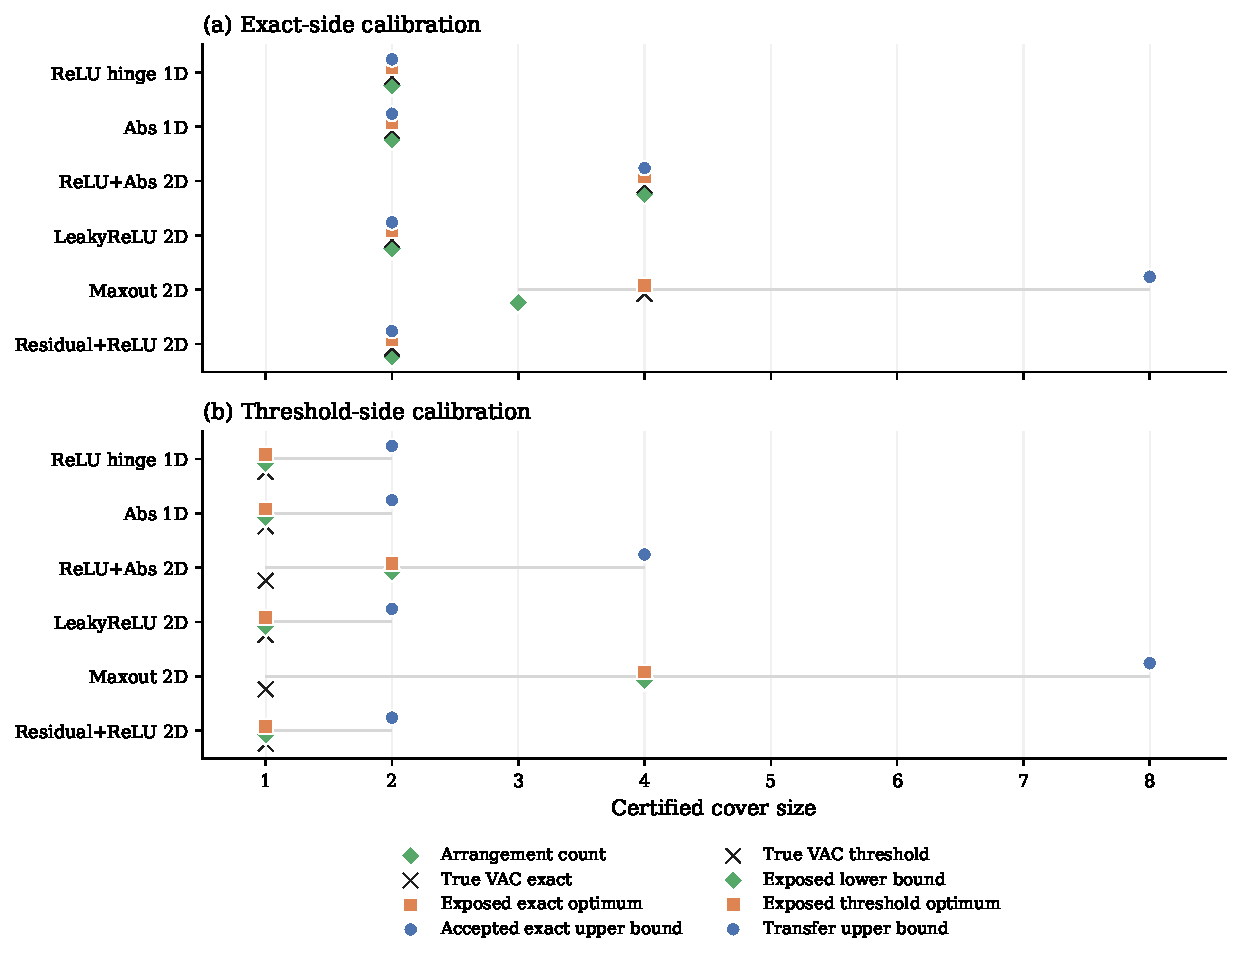
\includegraphics[width=0.94\textwidth]{figures/appendixI_goldtiny_calibration}
    \caption{Gold Tiny exhaustive calibration. Panel (a) compares arrangement count, true exact VAC in the guard language, the exposed exact optimum, and the accepted exactification upper bound. Five of the six tiny cases coincide on the exact side; the maxout case exhibits the intended separation \emph{arrangement count $<$ true exact VAC $<$ exactification upper bound}. Panel (b) compares true guard-language threshold VAC, the exposed lower bound, the exposed threshold optimum, and the transfer upper bound on canonical true-threshold tasks. This panel should be read as a language-calibration plot: exposed threshold quantities need not equal the true guard-language threshold VAC even on the tiny exhaustive suite.}
    \label{fig:appI-goldtiny-calibration}
\end{figure}

\clearpage
\subsection{Exact-Side Exactification and Compression}

Figure~\ref{fig:appI-exact-scaling} summarizes the constructive exactification upper bounds across the full benchmark suite. The accepted exact upper bound $U_{\mathrm{eq}}^{\mathrm{align}}$ grows with the number $H = |\mathcal H^\star|$ of compiled comparison hyperplanes, but on the saved bundle it stays well below the crude $2^H$ envelope. This is the main empirical counterpart of the finite exactification theorem: the theorem only guarantees a finite aligned split-tree upper bound, while the artifact shows that the realized upper bounds are much smaller than the coarsest combinatorial envelope on the benchmark families shipped here.

Figure~\ref{fig:appI-exact-compression} complements the scaling view with a compression view. The compression factor is
\[
\frac{U_{\mathrm{eq}}^{\mathrm{align}}}{\mathrm{OPT}_{\mathrm{eq}}^{\mathrm{exposed}}}.
\]
For Family A, Family B, and ThresholdStress, the median compression factor is $1.0\times$, meaning that the accepted exactification upper bound closely tracks the exposed exact optimum. Gold Tiny is also mostly at $1.0\times$, with the small maxout example producing the one visible exact-side gap. By contrast, SelectionStress is deliberately designed to enlarge the exposed candidate language while keeping the final semantic exact cover small, and the resulting median compression factor is $12.5\times$ with substantially larger outliers. This is the cleanest experimental manifestation of the paper's exact-side ``candidate exposure versus semantic optimum'' distinction.

\begin{figure}[t]
    \centering
    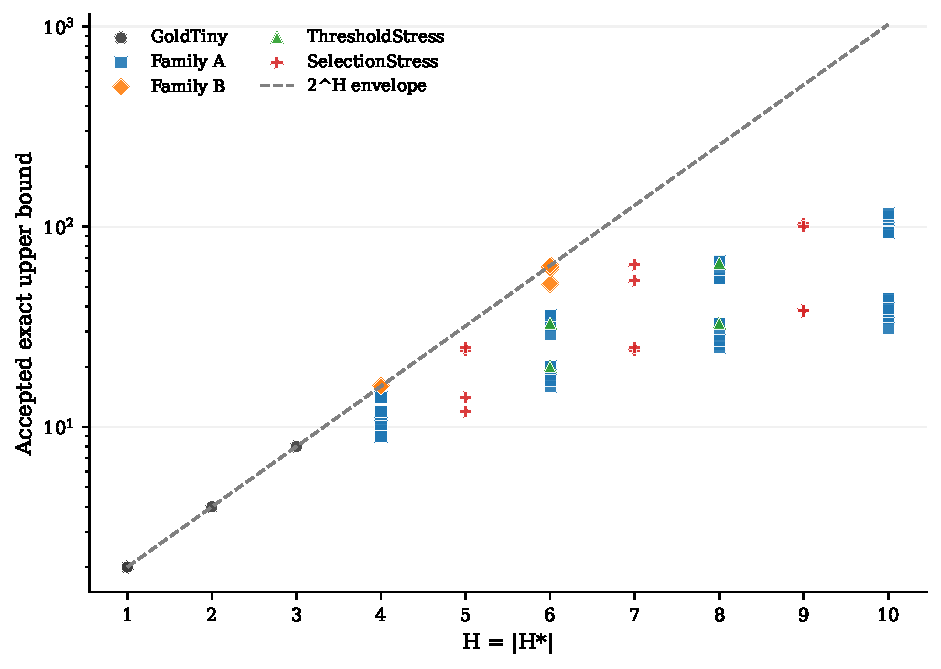
\includegraphics[width=0.78\textwidth]{figures/appendixI_exact_scaling}
    \caption{Exactification scaling across the full benchmark suite. Each point is one saved exact-side row. The dashed curve is the crude $2^H$ envelope. Accepted exact upper bounds grow with $H$, but remain far below the envelope on the shipped paper-facing bundle.}
    \label{fig:appI-exact-scaling}
\end{figure}

\begin{figure}[t]
    \centering
    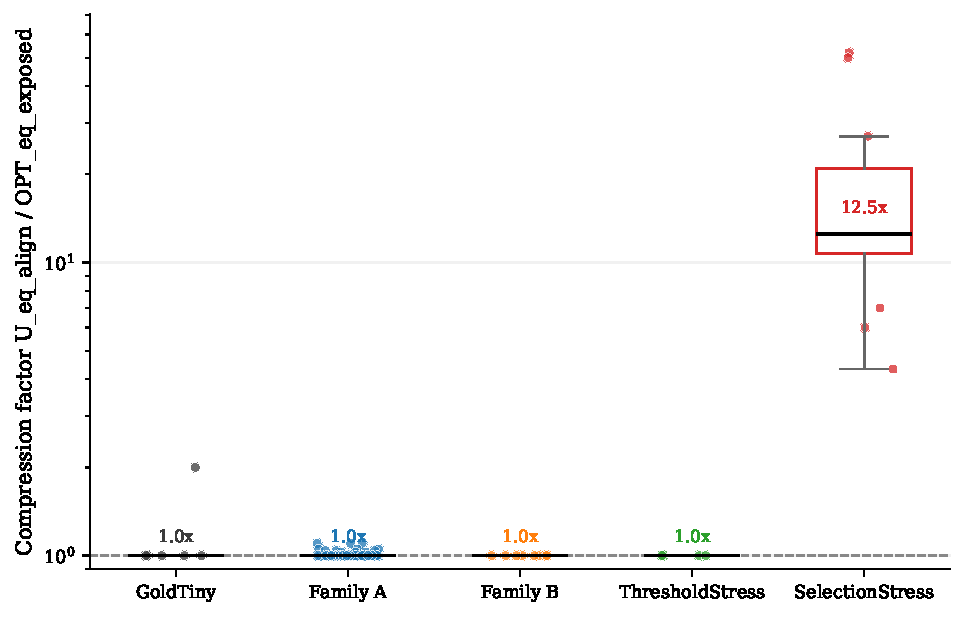
\includegraphics[width=0.80\textwidth]{figures/appendixI_exact_compression_by_family}
    \caption{Exact-side compression factor by family. The plotted quantity is $U_{\mathrm{eq}}^{\mathrm{align}} / \mathrm{OPT}_{\mathrm{eq}}^{\mathrm{exposed}}$. Family A, Family B, and ThresholdStress stay concentrated at $1.0\times$, while SelectionStress exhibits large exposed-language compression. Gold Tiny is almost entirely at $1.0\times$, with the maxout example providing the intended small deviation.}
    \label{fig:appI-exact-compression}
\end{figure}

\clearpage
\subsection{Threshold-Side Upper Bounds, Exposure, and Diagnostics}

The threshold side is organized around one canonical true-threshold task per instance together with one false control. The false controls are clean in the saved bundle: none of the 126 false-control rows admits a finite accepted threshold cover. On the positive side, Figure~\ref{fig:appI-threshold-gap} plots the transfer upper bound against the exposed threshold optimum for the canonical true tasks. Every point lies below the diagonal, exactly as expected from the transfer theorem: an accepted exact cover transfers to a threshold cover of no larger size.

The threshold story is more subtle than a blanket ``threshold is easier'' slogan. Figure~\ref{fig:appI-threshold-vs-exact} is included specifically to make that subtlety explicit. On Family A, Family B, Gold Tiny, and ThresholdStress, the exposed threshold optimum is typically below the exposed exact optimum. However, SelectionStress is intentionally a counterexample family: it targets exact-side cancellation/compression and therefore can have a much smaller exposed exact optimum while still requiring a larger threshold-side exposed cover in the bounded threshold language implemented by the artifact. The threshold section of the paper should therefore be written in the language-relative form used throughout the repository notes, not as a claim of universal threshold dominance.

Figure~\ref{fig:appI-threshold-stage} then isolates the threshold-stage exposure mechanism on the curated threshold subset. The conservative v3 default sets the parent-backtracking depth to zero, so the $D_{\mathrm{transfer}}$ and $+D_{\mathrm{parent}}$ stages are intentionally dormant controls. The visible gain arrives at the $+D_{\mathrm{drop}}$ stage: the median dictionary size increases from $38.0$ to $254.5$, while the median exposed threshold optimum decreases from $38.0$ to $19.5$. The median exposed lower bound stays at $16.0$, so the final stage is not merely adding vacuous candidates; it is exposing a strictly better cover language while remaining close to the certified lower-bound floor.

\begin{figure}[t]
    \centering
    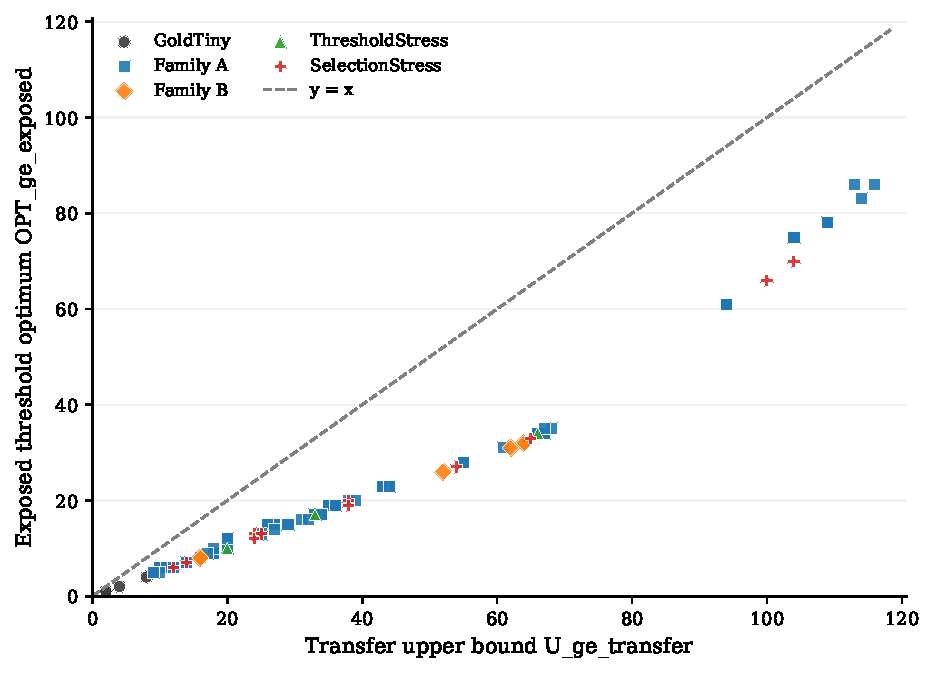
\includegraphics[width=0.80\textwidth]{figures/appendixI_threshold_transfer_gap}
    \caption{Transfer upper bound versus exposed threshold optimum on canonical true-threshold tasks. All points lie below the diagonal, as required by the exact-to-threshold transfer upper bound.}
    \label{fig:appI-threshold-gap}
\end{figure}

\begin{figure}[t]
    \centering
    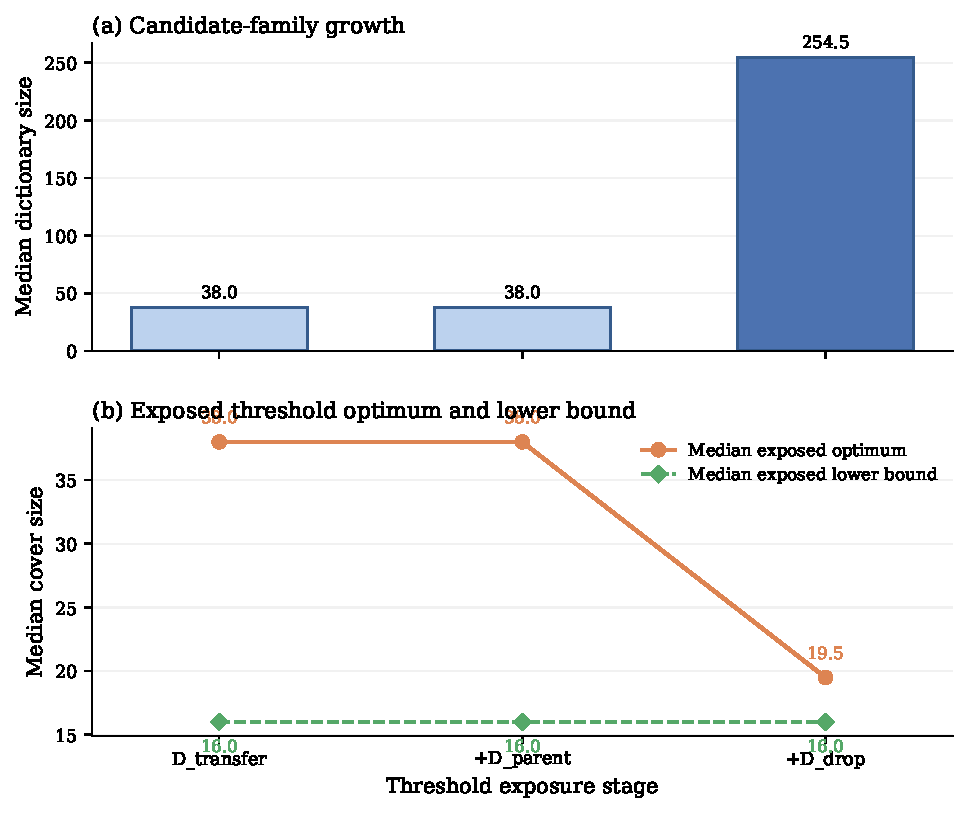
\includegraphics[width=0.80\textwidth]{figures/appendixI_threshold_stage_ablation}
    \caption{Threshold-stage ablation on the curated threshold subset. Under the conservative v3 default, parent backtracking is disabled, so $D_{\mathrm{transfer}}$ and $+D_{\mathrm{parent}}$ coincide. The $+D_{\mathrm{drop}}$ stage enlarges the exposed threshold dictionary and reduces the median exposed optimum from $38.0$ to $19.5$ while the median exposed lower bound remains at $16.0$.}
    \label{fig:appI-threshold-stage}
\end{figure}

\begin{figure}[t]
    \centering
    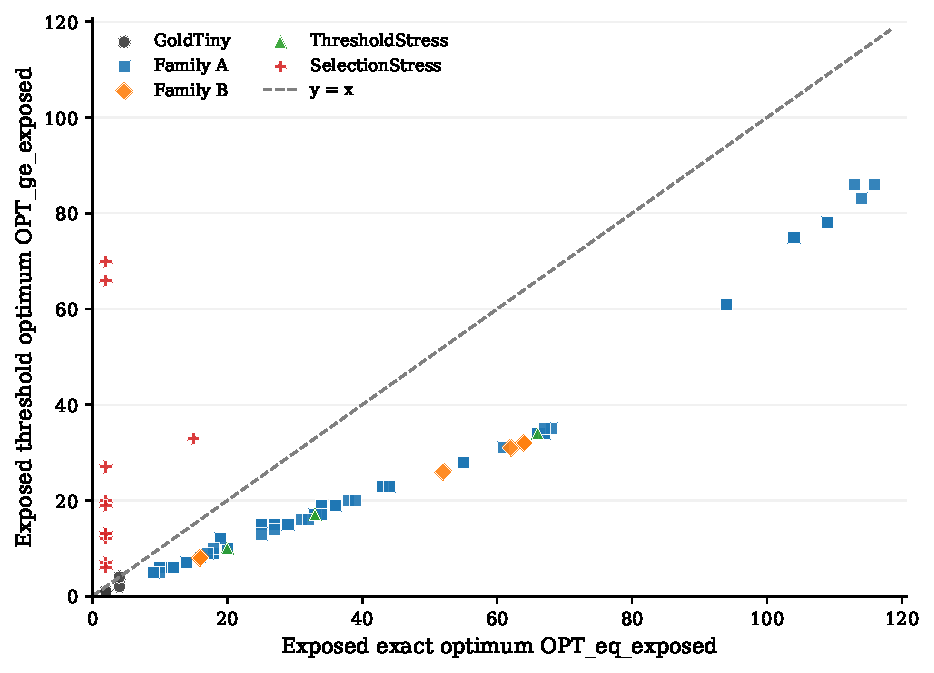
\includegraphics[width=0.80\textwidth]{figures/appendixI_threshold_vs_exact_diagnostic}
    \caption{Threshold-versus-exact diagnostic on the canonical true-threshold rows. Most benchmark families lie below the diagonal, while SelectionStress intentionally lies above it. Thus threshold exposed optima are not universally smaller than exact exposed optima; the comparison depends on the exposed candidate language and on the benchmark family.}
    \label{fig:appI-threshold-vs-exact}
\end{figure}

\clearpage
\subsection{Selection-Layer Exposure on Explicit Candidate Families}

The exact-side selection experiment is intentionally separated from the exactification scaling experiment. Its job is not to estimate unrestricted semantic hardness for every benchmark family. Its job is to show what happens after the pipeline has already exposed an explicit finite candidate family and the remaining problem is to select a smallest accepted subcover inside that family.

Figure~\ref{fig:appI-selection-stage} shows the stagewise behavior on the curated selection subset. The median dictionary size grows from $40.5$ at $D_{\mathrm{leaf}}$ to $145.0$ at $D_{\mathrm{leaf}} + D_{\mathrm{frag}}$, then to $224.0$ at $+D_{\mathrm{parent}}$, and finally to $586.0$ at $+D_{\mathrm{drop}}$. At the same time, the median exposed exact optimum stays at $40.5$ through the first two stages and then collapses to $3.0$ at the parent/drop stages. The qualitative lesson is that exposing more candidates can make the selection layer dramatically more informative before any theorem-level hardness statement is invoked.

The repository's SelectionStress family is deliberately targeted to make this phenomenon visible. Accordingly, Figure~\ref{fig:appI-selection-stage} should be interpreted as an explicit-dictionary stress demonstration rather than as a blanket empirical statement that selection is the dominant difficulty on every family. That scoped interpretation matches the theoretical hardness discussion in Section~\ref{sec:vac-minimization} and Appendix~\ref{app:dict-hardness}.

\begin{figure}[t]
    \centering
    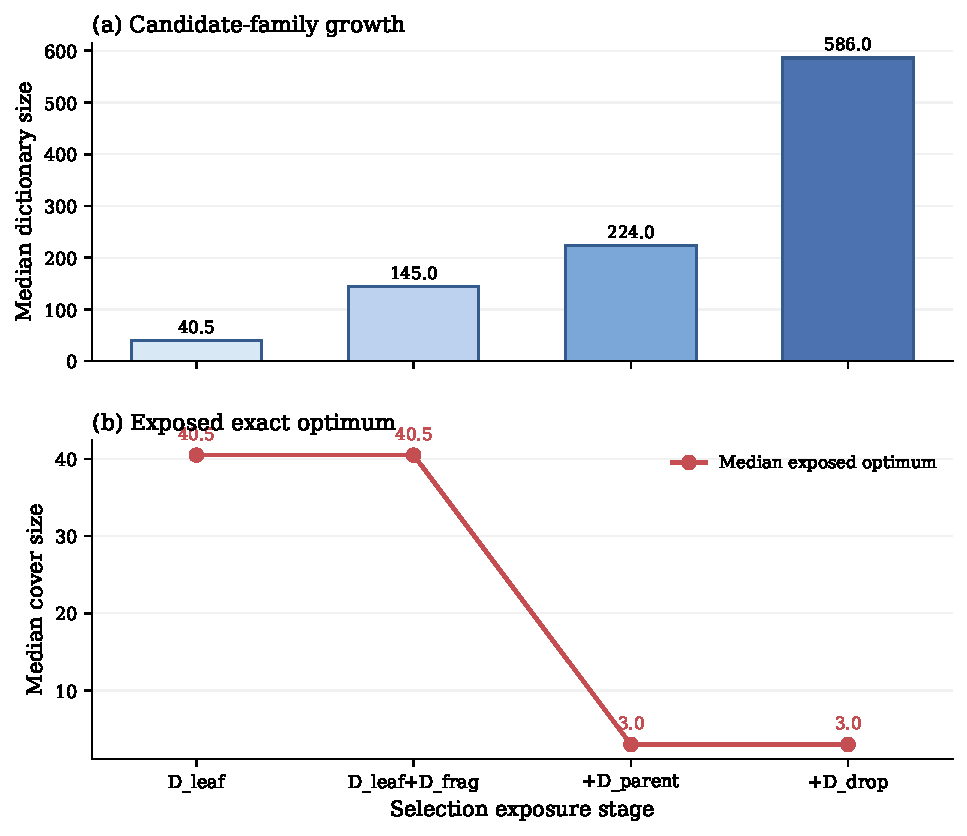
\includegraphics[width=0.80\textwidth]{figures/appendixI_selection_stage_ablation}
    \caption{Selection-stage ablation on the curated explicit-candidate subset. Candidate exposure grows from $D_{\mathrm{leaf}}$ to $+D_{\mathrm{drop}}$, while the median exposed exact optimum collapses from $40.5$ to $3.0$. This is a stress-family demonstration of selection-layer compression after candidate exposure, not a blanket claim about every benchmark family.}
    \label{fig:appI-selection-stage}
\end{figure}

\clearpage
\subsection{Realization-Side Payload, Checking Cost, and Runtime}

The realization figures separate the semantic proof payload from full engineering archives. This distinction is essential for interpreting the SCC/DL-facing part of the artifact. Figure~\ref{fig:appI-realization} shows that compact/core binary payload size is almost perfectly linear in proof-cell count, while archive bundles are much larger and vary strongly by family. On the saved bundle, the fitted core-byte slope is approximately $206$ bytes per proof cell, and the Pearson correlation between proof-cell count and compact/core binary size is about $0.995$. By contrast, the median archive-to-core ratio is only about $5.1\times$ on Gold Tiny but rises to roughly $21.6\times$ on Family A, $15.6\times$ on Family B, $18.5\times$ on ThresholdStress, and $251.7\times$ on SelectionStress. The archive should therefore be read as engineering overhead, not as a direct measure of semantic proof payload size.

Figure~\ref{fig:appI-core-check} shows the same near-linear behavior for checker runtime on compact/core payloads. The saved bundle stays below one millisecond for the core binary checker, with the largest observed values remaining around $0.6$ ms. Finally, Figure~\ref{fig:appI-generation-time} reports exactification generation time as a function of $H$. The paper-facing bundle is not designed as a maximal stress benchmark, yet it is still useful to record that the constructive exactification pass remains within a few seconds on all shipped instances. In the saved run, the largest generation times stay below approximately $6$ seconds.

Taken together, these figures support the main text's final empirical message: exactification yields observable finite exact covers with moderate constructive cost; threshold-side and selection-side exposure change the optimum before any hardness statement is applied; and compact/core proof realizations are the right object to compare at the realization layer, while full archive bundles should be reported separately.

\begin{figure}[t]
    \centering
    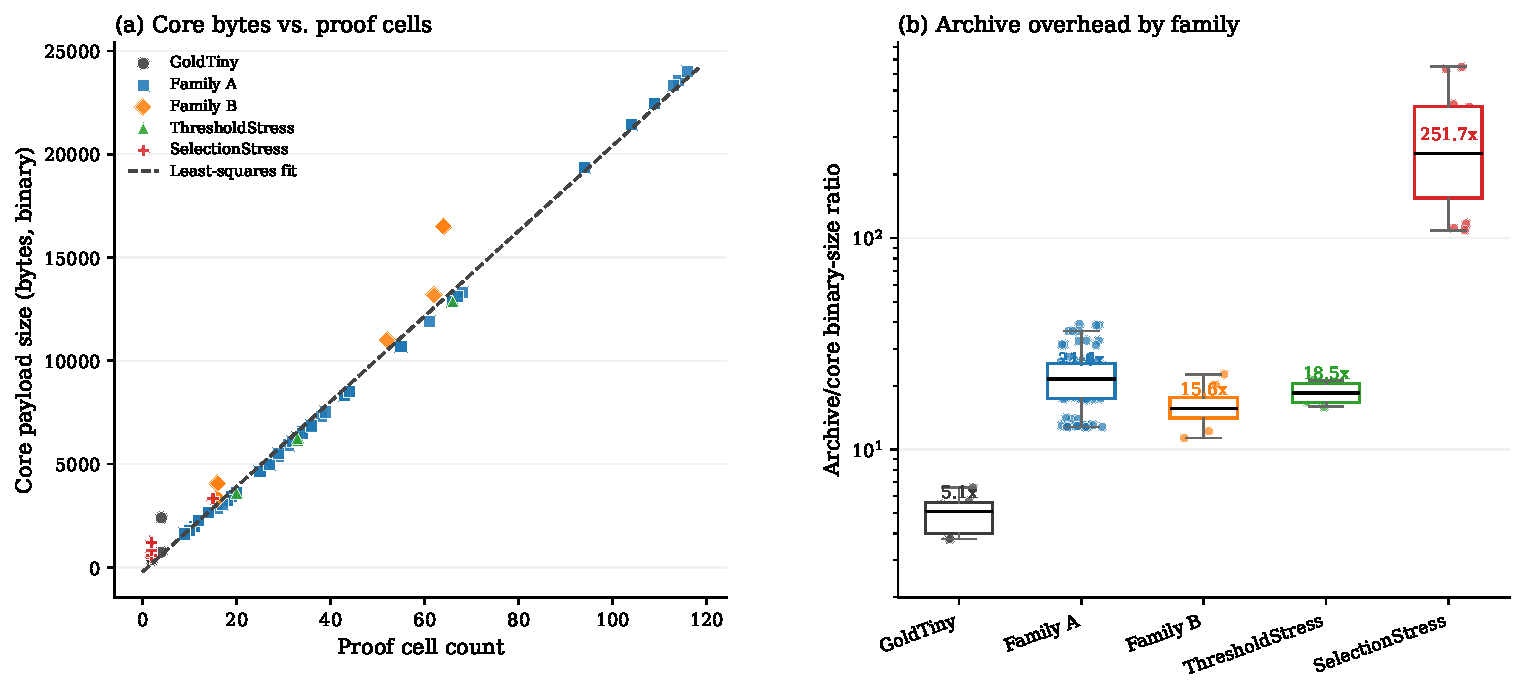
\includegraphics[width=\textwidth]{figures/appendixI_realization_dual}
    \caption{Realization-side payload metrics. Panel (a) shows near-linear scaling between proof-cell count and compact/core binary payload size. Panel (b) shows that archive bundles are much larger than compact/core payloads, especially on SelectionStress; archive size therefore should not be conflated with semantic proof payload size.}
    \label{fig:appI-realization}
\end{figure}

\begin{figure}[t]
    \centering
    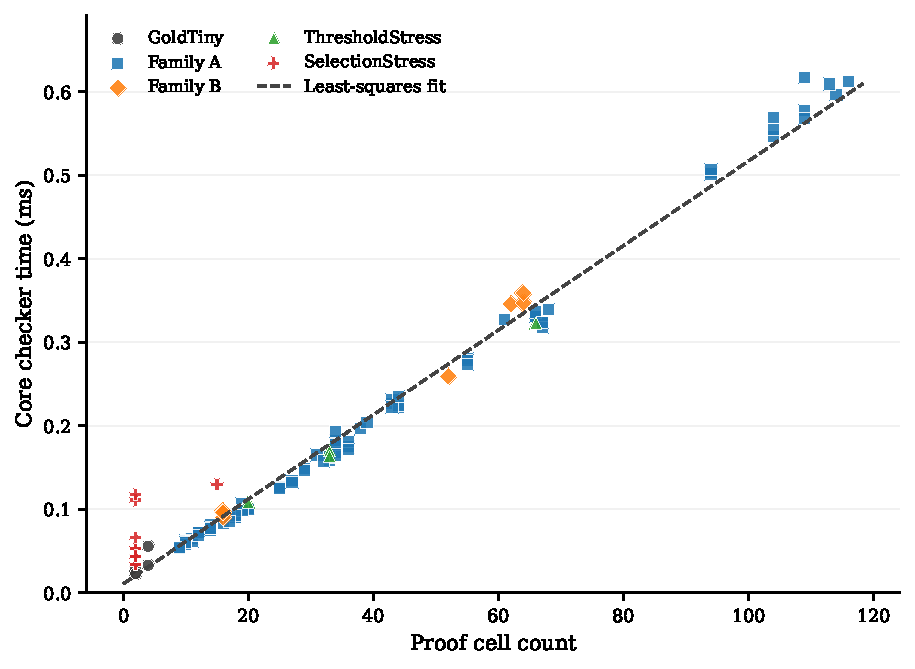
\includegraphics[width=0.80\textwidth]{figures/appendixI_core_checker_time}
    \caption{Compact/core checker time versus proof-cell count. Core checking remains sub-millisecond on the saved bundle and is close to linear in proof-cell count.}
    \label{fig:appI-core-check}
\end{figure}

\begin{figure}[t]
    \centering
    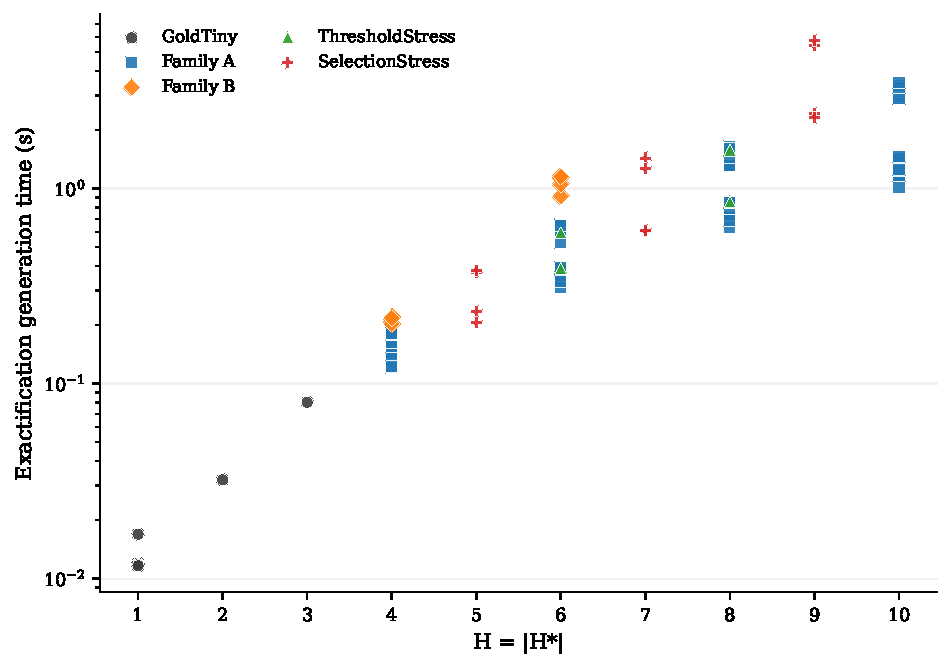
\includegraphics[width=0.80\textwidth]{figures/appendixI_generation_time}
    \caption{Exactification generation time versus $H = |\mathcal H^\star|$. The constructive exactification pass grows with problem size but remains within a few seconds on the saved paper-facing bundle.}
    \label{fig:appI-generation-time}
\end{figure}


\newpage

\end{document}
